\documentclass{book}
\usepackage[spanish]{babel}
\usepackage[T1]{fontenc}
\usepackage[utf8]{inputenc}
\usepackage{amsmath, amssymb}
\usepackage{dsfont}
\usepackage{graphics}
\usepackage{cases}
\usepackage{graphicx}
\usepackage{pgf}
\usepackage{epsfig}
\usepackage{amssymb}
\usepackage{multirow}
\usepackage{amstext}
\usepackage[ruled,vlined,lined]{algorithm2e}
\usepackage{listings}
\usepackage{amsmath}
\usepackage{epic}
\usepackage{epsfig}
\usepackage{fontenc}
\usepackage{framed,color}
\usepackage{palatino, url, multicol}



\begin{document}


\pagestyle{empty}

\begin{titlepage}
    \begin{center}
        \vspace*{1cm}
        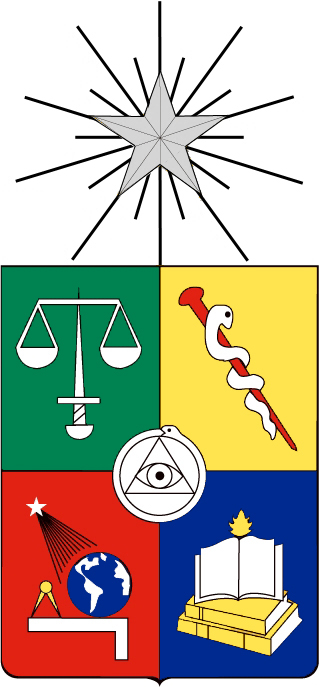
\includegraphics[width=2cm]{pics/escudocolor.png} % Replace "pics/escudocolor.png" with the filename and path of your logo image
        \vspace{1cm}
        
        {\Huge\textbf{Universidad de Chile}} \\
        \vspace{0.5cm}
        {\Large Departamento de Ciencias de la Computación} \\
        \vspace{2cm}
        
        {\Huge\textbf{Procesamiento de Lenguaje Natural}} \\
        \vspace{0.5cm}
        {\Large Apuntes de Clases} \\
        \vspace{2cm}
        
        {\Large Felipe Bravo-Márquez} \\
        \vspace{2cm}
        
        {\large \today}
    \end{center}
\end{titlepage}

\newpage
\thispagestyle{empty}

\newpage
\pagenumbering{roman}

\tableofcontents 
\newpage

\listoftables
\newpage
\listoffigures
\newpage


\thispagestyle{empty}


\pagenumbering{arabic}

%..................................................



\chapter{Introducción}
\label{cap:intro}


El volumen de datos textuales digitalizados que se genera cada día es enorme (por ejemplo, la web, redes sociales, registros médicos, libros digitalizados). Por lo tanto, también crece la necesidad de traducir, analizar y gestionar esta avalancha de palabras y texto.

El procesamiento del lenguaje natural (PLN) es el campo que se encarga de diseñar métodos y algoritmos que toman como entrada o producen como salida datos de \textbf{lenguaje natural} no estructurado \cite{goldberg2017neural}. El PLN se centra en el diseño y análisis de algoritmos computacionales y representaciones para procesar el lenguaje humano \cite{jacobbook}.





Una tarea común de PLN es el Reconocimiento de Entidades Nombradas (NER, por sus siglas en inglés). Por ejemplo:

\begin{figure}[h]
	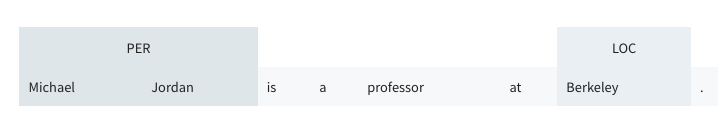
\includegraphics[scale=0.4]{pics/NER.png}
	\caption{Reconocimiento de Entidades Nombradas}
\end{figure}

El lenguaje humano es altamente ambiguo, como en las frases: "Comí pizza con amigos", "Comí pizza con aceitunas" o "Comí pizza con un tenedor". Además, el lenguaje está en constante cambio y evolución, como ocurre con los hashtags en Twitter.

\section{PLN y Lingüística Computacional}
PLN suele confundirse con otra disciplina hermana llamada Lingüística Computacional (LC). Si bien ambas están estrechamente relacionadas, tienen un foco distinto. La LC busca responder preguntas fundamentales sobre el lenguaje mediante el uso de la computación, es decir, cómo entendemos el lenguaje, cómo producimos lenguaje o cómo aprendemos lenguaje. Mientras que en PLN el foco está en resolver problemas específicos, tales como las transcripción automática del habla, la traducción automática, la extracción de información de documentos y el análisis de opiniones en redes sociales. Es importante señalar que en PLN, el éxito de una solución se mide en base métricas concretas (Ej: qué tan similar es la traducción automática a una hecha por un humano) independientemente si el modelo hace uso de alguna teoría lingüística.



El procesamiento del lenguaje natural (PLN) desarrolla métodos para resolver problemas prácticos relacionados con el lenguaje \cite{JohnsonMLSS}.

Algunos ejemplos son:

\begin{itemize}
  \item Reconocimiento automático del habla.
  \item Traducción automática.
  \item Extracción de información de documentos.
\end{itemize}

La lingüística computacional (LC) estudia los procesos computacionales subyacentes al lenguaje (humano).

\begin{itemize}
  \item ¿Cómo comprendemos el lenguaje?
  \item ¿Cómo producimos el lenguaje?
  \item ¿Cómo aprendemos el lenguaje?
\end{itemize}

El PLN y la LC utilizan métodos y modelos similares.


Aunque existe una superposición sustancial, hay una diferencia importante en el enfoque. La LC se centra en la lingüística respaldada por métodos computacionales (similar a la biología computacional o la astronomía computacional). En lingüística, el lenguaje es el objeto de estudio. El PLN se centra en resolver tareas bien definidas relacionadas con el lenguaje humano (como la traducción, la respuesta a consultas, las conversaciones). Si bien los conocimientos lingüísticos fundamentales pueden ser cruciales para realizar estas tareas, el éxito se mide en función de si y cómo se logra el objetivo (según una métrica de evaluación) \cite{jacobbook}.



El procesamiento del lenguaje natural y la lingüística computacional están estrechamente relacionados y se superponen en muchos aspectos. Ambos campos utilizan métodos y modelos similares para abordar problemas relacionados con el lenguaje humano. Sin embargo, la diferencia principal radica en el enfoque: la lingüística computacional se centra en la lingüística respaldada por métodos computacionales, mientras que el procesamiento del lenguaje natural se centra en resolver tareas prácticas relacionadas con el lenguaje. Ambos campos son fundamentales para comprender y aprovechar el poder del lenguaje humano en la era digital.


\section{Niveles de descripción lingüística}

El campo de la \textbf{descripción lingüística} abarca diferentes niveles:

\begin{itemize}
  \item \textbf{Fonética y fonología:} estudio de los sonidos del habla.
  \item \textbf{Morfología:} estudio de la estructura de las palabras.
  \item \textbf{Sintaxis:} estudio de la estructura de las oraciones.
  \item \textbf{Semántica:} estudio del significado de las palabras y oraciones.
  \item \textbf{Pragmática:} estudio del uso del lenguaje en el contexto.
\end{itemize}

El PLN puede abordar tareas en cada uno de estos niveles, pero a menudo se enfoca en niveles más altos de representación y comprensión.




\subsection{Fonética}

La fonética es la rama de la lingüística que se ocupa del estudio de los sonidos del lenguaje. Examina los órganos utilizados en la producción de sonidos, como la boca, la lengua, la garganta, la nariz, los labios y el paladar. Los sonidos del lenguaje se dividen en vocales y consonantes. Las vocales se producen con poca restricción del flujo de aire desde los pulmones, mientras que las consonantes implican alguna restricción o cierre en el tracto vocal \cite{JohnsonMLSS, fromkin2018introduction}. Además, el Alfabeto Fonético Internacional (AFI) proporciona una notación alfabética para representar los sonidos fonéticos.

\subsection{Fonología}

La fonología se centra en el estudio de cómo los sonidos del habla forman patrones y construyen significado. Los fonemas son las unidades básicas de sonido que diferencian el significado de las palabras. Por ejemplo, en inglés, la "p" y la "b" son fonemas distintos porque cambian el significado de las palabras en las que se encuentran. La fonología también examina las variaciones en la pronunciación de los sonidos en diferentes contextos y dialectos \cite{fromkin2018introduction}.

\subsection{Morfología}

La morfología se ocupa del estudio de la estructura interna de las palabras. Los morfemas son las unidades mínimas de significado que componen las palabras. Por ejemplo, en la palabra "deshacer", los morfemas son "des-", "hacer" y "-er". La morfología también se interesa por los procesos de formación de palabras, como la derivación, donde se agregan prefijos o sufijos a una palabra existente para formar una nueva palabra con un significado diferente \cite{JohnsonMLSS}.

\begin{itemize}
\item La morfología estudia la estructura de las palabras (por ejemplo, re+estructur+ando, in+olvid+able) \cite{JohnsonMLSS}
\item Morfema: el término lingüístico para la unidad más elemental de forma gramatical \cite{fromkin2018introduction}. Por ejemplo, morfología = morf + ología (la ciencia de).
\item Morfología derivativa: proceso de formar una nueva palabra a partir de una palabra existente, a menudo mediante la adición de un prefijo o sufijo.
\item La morfología derivativa exhibe una estructura jerárquica. Ejemplo: re+vital+iz+ación
\begin{figure}[h]
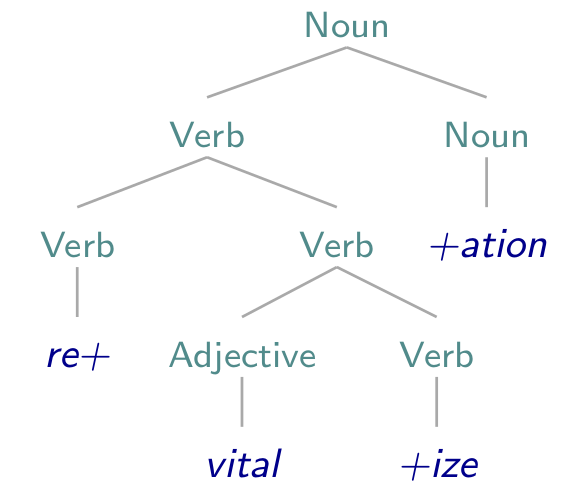
\includegraphics[scale = 0.2]{pics/morphology.png}
\end{figure}
\item El sufijo generalmente determina la categoría sintáctica (part-of-speech) de la palabra derivada.
\end{itemize}

\subsection{Sintaxis}

La sintaxis es el estudio de cómo las palabras se combinan para formar frases y oraciones gramaticales. Examina las reglas y estructuras que determinan la organización de las palabras en una oración y cómo influyen en el significado. La sintaxis también se ocupa de la relación entre las palabras y las funciones que desempeñan dentro de una oración. Por ejemplo, en la oración "El perro persigue al gato", "el perro" es el sujeto, "persigue" es el verbo y "al gato" es el complemento directo \cite{JohnsonMLSS}.

\begin{itemize}
\item La sintaxis estudia las formas en que las palabras se combinan para formar frases y oraciones \cite{JohnsonMLSS}
\begin{figure}[h]
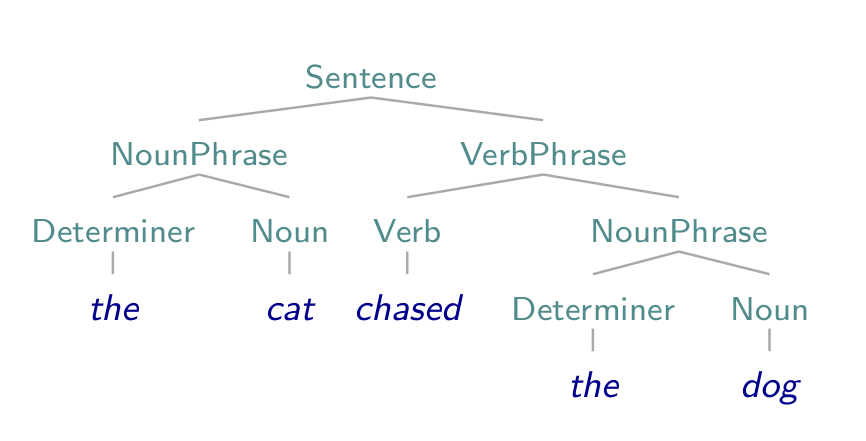
\includegraphics[scale = 0.3]{pics/parseTree1.png}
\end{figure}
\item El análisis sintáctico ayuda a identificar \textbf{quién hizo qué a quién}, un paso clave para comprender una oración.
\end{itemize}


\subsection{Semántica}

La semántica es el estudio del significado de las palabras, frases y oraciones, examinando cómo se construye e interpreta este significado en el contexto del lenguaje. Además, la semántica se interesa por los roles semánticos, que indican la función de cada entidad en una oración. Por ejemplo, en la oración "El niño cortó la cuerda con una navaja", "el niño" es el agente, "la cuerda" es el tema y "una navaja" es el instrumento \cite{JohnsonMLSS}.

La semántica se enfoca en el significado de las palabras, frases y oraciones. Estudia cómo se construye e interpreta este significado en el contexto del lenguaje. Además, dentro de la semántica, se analizan los roles semánticos, los cuales indican la función que desempeña cada entidad en una oración. Por ejemplo, en la oración "El niño cortó la cuerda con una navaja", se identifican distintos roles semánticos: "el niño" como el agente, "la cuerda" como el tema y "una navaja" como el instrumento utilizado \cite{JohnsonMLSS}.


En resumen:
\begin{itemize}
\item La semántica estudia el significado de las palabras, frases y oraciones \cite{JohnsonMLSS}.
\item Dentro de la semántica, se analizan los roles semánticos, que indican el papel desempeñado por cada entidad en una oración.
\item Algunos ejemplos de roles semánticos son: \textcolor[rgb]{0.00,0.00,1.00}{\textbf{agente}} (la entidad que realiza la acción), \textcolor[rgb]{1.00,0.00,0.00}{\textbf{tema}} (la entidad involucrada en la acción) y \textcolor[rgb]{0.00,1.00,0.00}{\textbf{instrumento}} (otra entidad utilizada por el agente para llevar a cabo la acción).
\item En la oración "El niño cortó la cuerda con una navaja", se puede identificar el agente como \textcolor[rgb]{0.00,0.00,1.00}{\textbf{el niño}}, el tema como \textcolor[rgb]{1.00,0.00,0.00}{\textbf{la cuerda}} y el instrumento como \textcolor[rgb]{0.00,1.00,0.00}{\textbf{una navaja}}.
\item Además de los roles semánticos, la semántica también abarca las relaciones léxicas, que son las relaciones entre diferentes palabras \cite{yule2016study}.
\item Algunos ejemplos de relaciones léxicas incluyen la sinonimia (conceal/hide), la antonimia (shallow/deep) y la hiponimia (perro/animal).
\end{itemize}


\subsection{Pragmática}

La pragmática se centra en cómo el contexto influye en la interpretación y el significado de las expresiones lingüísticas. Examina cómo se utilizan las expresiones lingüísticas en situaciones reales y cómo los hablantes interpretan el significado implícito. Por ejemplo, la oración "Hace frío aquí" puede interpretarse como una sugerencia implícita de cerrar las ventanas \cite{fromkin2018introduction}.


\section{Procesamiento del Lenguaje Natural y Aprendizaje Automático}

Comprender y producir el lenguaje computacionalmente es extremadamente complejo.  La tecnología más exitosa actualmente para abordar PLN es el aprendizaje automático supervisado que consiste en una familia de algoritmos que “aprenden” a construir la respuesta del problema en cuestión en base a encontrar patrones en datos de entrenamiento etiquetados. Por ejemplo, si queremos tener un modelo que nos diga si un tweet tiene un sentimiento positivo o negativo respecto a un producto, primero necesito  etiquetar manualmente un conjunto de tweets con su sentimiento asociado. Luego debo entrenar un algoritmo de aprendizaje sobre estos datos para poder predecir de manera automática el sentimiento asociado a tweets desconocidos. Como se podrán imaginar, el etiquetado de datos es una parte fundamental de la solución y puede ser un proceso muy costoso, especialmente cuando se requiere conocimiento especializado para definir la etiqueta.

Aunque los seres humanos somos grandes usuarios del lenguaje, también somos muy malos para comprender y describir formalmente las reglas que rigen el lenguaje.

Entender y producir lenguaje utilizando computadoras es altamente desafiante. Los métodos más conocidos para lidiar con datos de lenguaje se basan en el aprendizaje automático supervisado.

El aprendizaje automático supervisado consiste en intentar inferir patrones y regularidades a partir de un conjunto de pares de entrada y salida preanotados (también conocido como conjunto de datos de entrenamiento).

\paragraph{Conjunto de Datos de Entrenamiento: Datos de NER CoNLL-2003}

Cada línea contiene un token, una etiqueta de parte de la oración, una etiqueta de sintagma y una etiqueta de entidad nombrada.
\begin{center}
\begin{verbatim}
U.N.         NNP  I-NP  I-ORG
official     NN   I-NP  O
Ekeus        NNP  I-NP  I-PER
heads        VBZ  I-VP  O
for          IN   I-PP  O
Baghdad      NNP  I-NP  I-LOC
.            .    O     O
\end{verbatim}
\end{center}

\footnotemark{Fuente: \url{https://www.clips.uantwerpen.be/conll2003/ner/}}

\section{Desafíos del Lenguaje}

Existen tres propiedades desafiantes del lenguaje: la discreción, la composicionalidad y la dispersión.

\textbf{Discreción}: no podemos inferir la relación entre dos palabras a partir de las letras que las componen (por ejemplo, hamburguesa y pizza).

\textbf{Composicionalidad}: el significado de una oración va más allá del significado individual de sus palabras.

\textbf{Dispersión}: la forma en que las palabras (símbolos discretos) pueden combinarse para formar significados es prácticamente infinita.



\section{Ejemplo de tareas NLP}


\paragraph{Clasificación de temas}

La clasificación de temas es una tarea de Procesamiento del Lenguaje Natural (PLN) en la cual se asigna a un documento una de varias categorías, como deportes, política, cotilleos o economía. Las palabras presentes en los documentos brindan pistas importantes sobre su tema. Sin embargo, redactar reglas para esta tarea es un desafío debido a la complejidad del lenguaje. La anotación de datos, en la cual los lectores clasifican los documentos por temas, puede ayudar a generar conjuntos de datos de entrenamiento para algoritmos de aprendizaje automático supervisado. Estos algoritmos aprenden patrones de uso de palabras que facilitan la categorización de los documentos.

\begin{itemize}
\item Clasificar un documento en una de las cuatro categorías: Deportes, Política, Cotilleos y Economía.
\item Las palabras en los documentos proporcionan indicios muy sólidos.
\item ¿Qué palabras brindan qué indicios?
\item Elaborar reglas para esta tarea resulta bastante desafiante.
\item No obstante, los lectores pueden categorizar fácilmente varios documentos según su tema (anotación de datos).
\item Un algoritmo de aprendizaje automático supervisado puede identificar los patrones de uso de palabras que ayudan a categorizar los documentos.
\end{itemize}
\paragraph{Análisis de Sentimiento}

El análisis de sentimientos se refiere a la aplicación de técnicas de Procesamiento del Lenguaje Natural (PLN) para identificar y extraer información subjetiva de conjuntos de datos textuales. Un desafío común en el análisis de sentimientos es la clasificación de la polaridad a nivel de mensaje (MPC), donde las frases se clasifican automáticamente en categorías positivas, negativas o neutrales. Las soluciones más avanzadas utilizan modelos de aprendizaje automático supervisado entrenados con ejemplos anotados manualmente.

En este tipo de clasificación, es habitual emplear el aprendizaje supervisado, siendo las Máquinas de Vectores de Soporte (SVM) una opción popular. El objetivo de las SVM es encontrar un hiperplano que separe las clases con el margen máximo, logrando la mejor separación entre las clases positivas, negativas y neutrales \cite{jacobbook}.

\begin{itemize}
  \item Aplicación de técnicas de \textbf{PLN} para identificar y extraer información subjetiva de conjuntos de datos textuales.
  \item Clasificación automática de frases en las categorías \textcolor[rgb]{0.00,0.00,1.00}{\textbf{positiva}}, \textcolor[rgb]{1.00,0.00,0.00}{\textbf{negativa}} o \textcolor[rgb]{0.00,1.00,0.00}{\textbf{neutral}}.

     \begin{figure}[h]
        	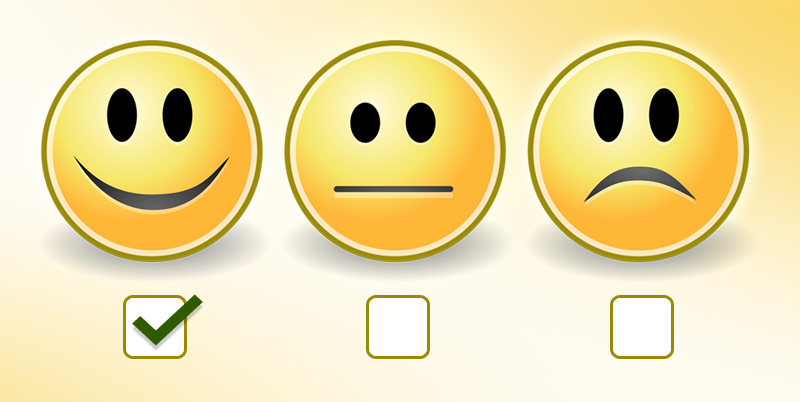
\includegraphics[scale = 0.15]{pics/sent.png}
        \end{figure}

  \item Las soluciones más avanzadas emplean modelos de aprendizaje automático \textbf{supervisado}, entrenados con ejemplos \textbf{anotados manualmente} \cite{Mohammad2013}.
\end{itemize}


\begin{figure}[h]
        	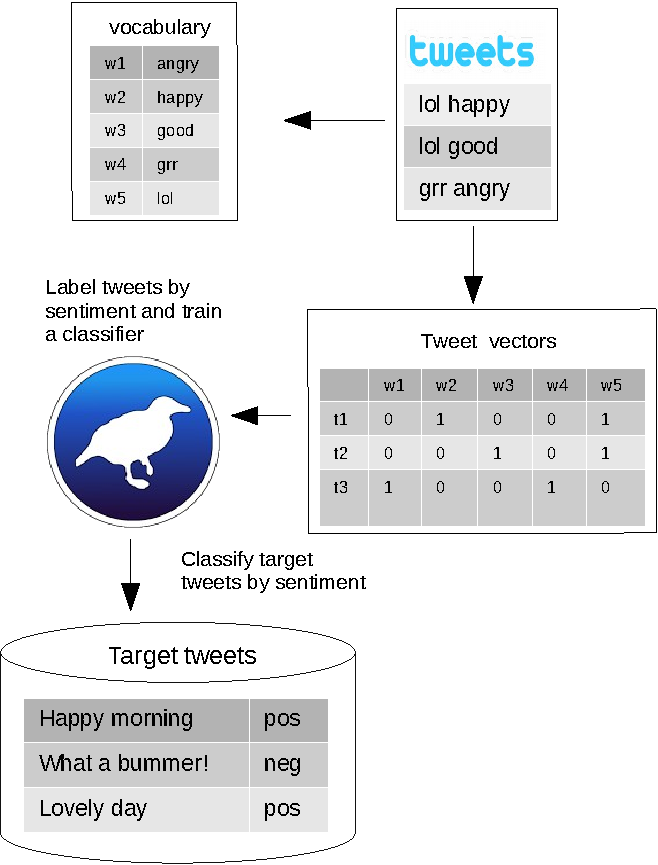
\includegraphics[scale = 0.5]{pics/bagOfwordsClassification.pdf}
        \end{figure}


\begin{itemize}


\item Idea: Encontrar un hiperplano que separe las clases con el margen máximo (mayor separación).

     \begin{figure}[h]
        	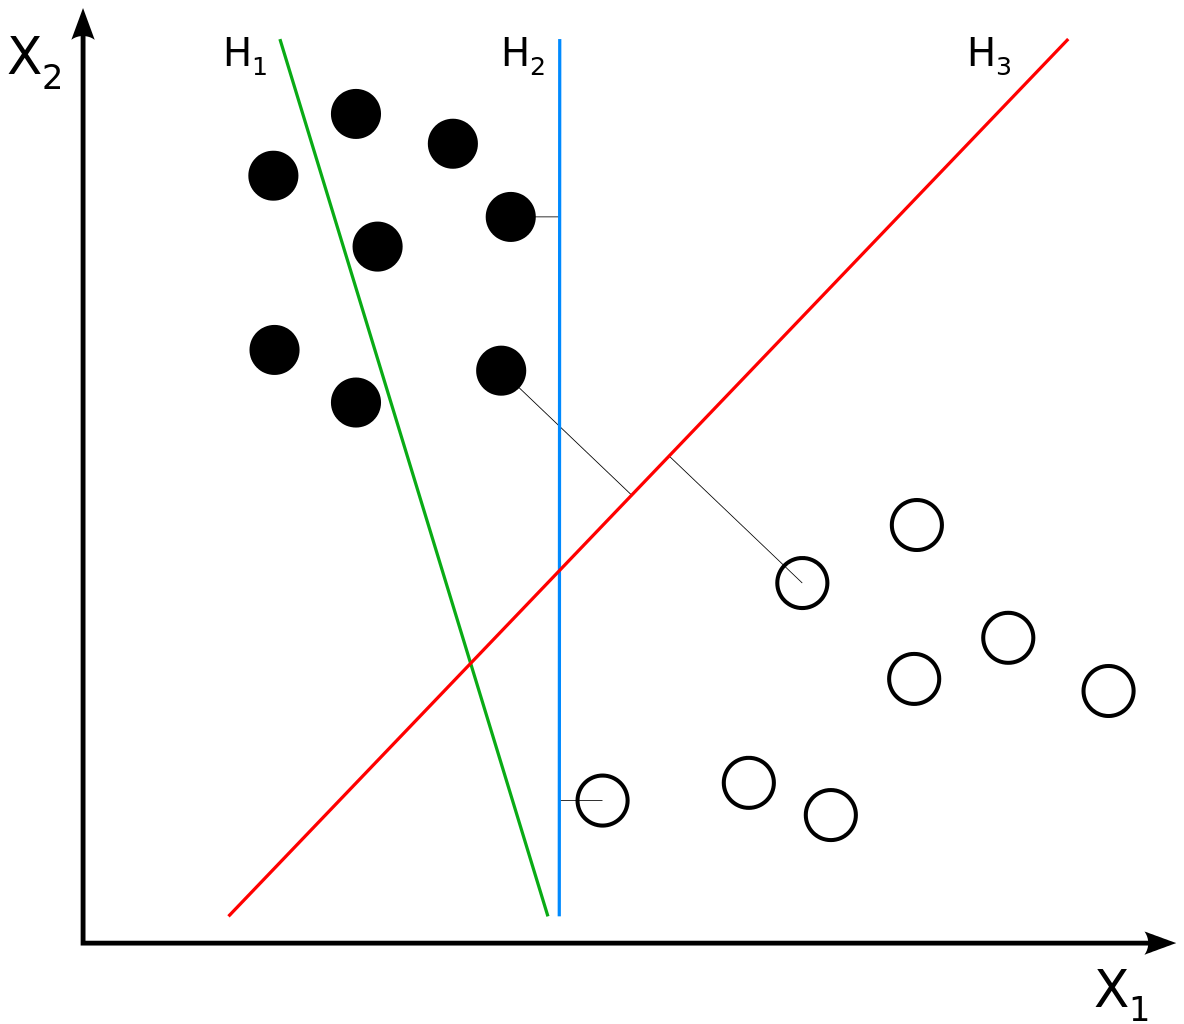
\includegraphics[scale = 0.15]{pics/SVM.png}
        \end{figure}

\item $H_3$ separa las clases con el margen máximo.

\end{itemize}


\subsection{Lingüística y Procesamiento del Lenguaje Natural (PNL)}

El conocimiento de las estructuras lingüísticas es fundamental para el diseño de características y el análisis de errores en el Procesamiento del Lenguaje Natural (PNL). Los enfoques de aprendizaje automático en PNL se basan en características que describen y generalizan las instancias de uso del lenguaje. El conocimiento lingüístico orienta la selección y el diseño de estas características, ayudando al algoritmo de aprendizaje automático a encontrar correlaciones entre el uso del lenguaje y las etiquetas objetivo \cite{bender2013linguistic}.

\begin{itemize}
  \item El conocimiento de las estructuras lingüísticas es importante para el diseño de características y el análisis de errores en PNL \cite{bender2013linguistic}.
  \item Los enfoques de aprendizaje automático en PNL requieren características que puedan describir y generalizar el uso del lenguaje.
  \item El objetivo es guiar al algoritmo de aprendizaje automático para encontrar correlaciones entre el uso del lenguaje y el conjunto de etiquetas objetivo.
  \item El conocimiento sobre las estructuras lingüísticas puede influir en el diseño de características para los enfoques de aprendizaje automático en PNL.
\end{itemize}

El PNL plantea diversos desafíos, como los costos de anotación, las variaciones de dominio y la necesidad de actualizaciones continuas. La anotación manual requiere mucho trabajo y tiempo. Las variaciones de dominio implican aprender patrones diferentes para diferentes corpus de texto. Los modelos entrenados en un dominio pueden no funcionar bien en otro. Además, los modelos de PNL pueden volverse obsoletos a medida que el uso del lenguaje evoluciona con el tiempo.




\section{Desafíos en el Procesamiento del Lenguaje Natural (PNL)}

\begin{itemize}
   \item \textbf{Costos de Anotación}: la anotación manual es \textbf{laboriosa} y \textbf{consume mucho tiempo}.
   \item \textbf{Variaciones de Dominio}: el patrón que queremos aprender puede variar de un corpus a otro (por ejemplo, deportes, política).

   \item ¡Un modelo entrenado con datos anotados de un dominio no necesariamente funcionará en otro!
   \item Los modelos entrenados pueden quedar desactualizados con el tiempo (por ejemplo, nuevos hashtags).
\end{itemize}

\paragraph{Variación de Dominio en el Análisis de Sentimiento}
\begin{enumerate}
   \item Para mí, la cola era bastante \textcolor[rgb]{0.00,0.00,1.00}{\textbf{pequeña}} y solo tuve que esperar unos 20 minutos, ¡pero valió la pena! :D @raynwise
   \item Extraña espacialidad en Stuttgart. La habitación del hotel es tan \textcolor[rgb]{1.00,0.00,0.00}{\textbf{pequeña}} que apenas puedo moverme, pero los alrededores son inhumanamente vastos y largos bajo construcción.
\end{enumerate}

\paragraph{Superando los costos de anotación de datos}
Supervisión Distant:
\begin{itemize}
   \item Etiquetar automáticamente datos no etiquetados (\textbf{API de Twitter}) utilizando un método heurístico.
   \item \textbf{Enfoque de Anotación de Emoticonos (EAA)}: los tweets con emoticonos positivos \textcolor[rgb]{0.00,0.00,1.00}{\textbf{:)}} o negativos \textcolor[rgb]{1.00,0.00,0.00}{\textbf{:(}} se etiquetan según la polaridad indicada por el emoticono~\cite{Read2005}.
   \item El emoticono se \textbf{elimina} del contenido.
   \item Este enfoque también se ha ampliado utilizando hashtags como \#anger y emojis.
   \item No es trivial encontrar técnicas de supervisión distante para todo tipo de problemas de PNL.
\end{itemize}

\paragraph{Crowdsourcing}
\begin{itemize}
   \item Confiar en servicios como \textbf{Amazon Mechanical Turk} o \textbf{Crowdflower} para solicitar a la \textbf{multitud} que anote datos.
   \item Esto puede resultar costoso.
   \item Es difícil garantizar la calidad de las anotaciones.
\end{itemize}

\section{Estudio de caso: Clasificación de sentimientos en tweets}

\begin{itemize}
   \item En 2013, el taller de Evaluación Semántica (SemEval) organizó la tarea de "Análisis de sentimientos en Twitter" \cite{Semeval2013}.
   \item La tarea se dividió en dos sub-tareas: el nivel de expresión y el nivel del mensaje.
   \item Nivel de expresión: se centró en determinar la polaridad del sentimiento de un mensaje según una entidad marcada dentro de su contenido.
   \item Nivel del mensaje: se debía determinar la polaridad según el mensaje en general.
   \item Los organizadores lanzaron conjuntos de datos de entrenamiento y prueba para ambas tareas \cite{Semeval2013}.
\end{itemize}

\paragraph{El sistema NRC}
\begin{itemize}
   \item El equipo que logró el mejor rendimiento en ambas tareas, entre 44 equipos, fue el equipo \emph{NRC-Canada} \cite{Mohammad2013}.
   \item El equipo propuso un enfoque supervisado utilizando un clasificador SVM lineal con las siguientes características hechas a mano para representar los tweets:
   \begin{enumerate}
      \item N-gramas de palabras.
      \item N-gramas de caracteres.
      \item Etiquetas de partes del discurso.
      \item Agrupaciones de palabras entrenadas con el método de agrupamiento de Brown \cite{brown1992class}.
      \item El número de palabras alargadas (palabras con un carácter repetido más de dos veces).
      \item El número de palabras con todas las letras en mayúscula.
      \item La presencia de emoticonos positivos o negativos.
      \item El número de negaciones individuales.
      \item El número de secuencias contiguas de puntos, signos de interrogación y signos de exclamación.
      \item Características derivadas de lexicones de polaridad \cite{Mohammad2013}. Dos de estos lexicones se generaron utilizando el método PMI a partir de tweets anotados con hashtags y emoticonos.
   \end{enumerate}
\end{itemize}

\section{Ingeniería de características y Aprendizaje Profundo}

\begin{itemize}
   \item Hasta 2014, la mayoría de los sistemas de PNL de última generación se basaban en ingeniería de características + modelos de aprendizaje automático superficiales (por ejemplo, SVM, HMM).
   \item Diseñar las características de un sistema de PNL ganador requiere mucho conocimiento específico del dominio.
   \item El sistema NRC se construyó antes de que el aprendizaje profundo se hiciera popular en PNL.
   \item Por otro lado, los sistemas de Aprendizaje Profundo se basan en redes neuronales para aprender automáticamente buenas representaciones.
\end{itemize}

\paragraph{Ingeniería de características y Aprendizaje Profundo}

\begin{figure}[h]
   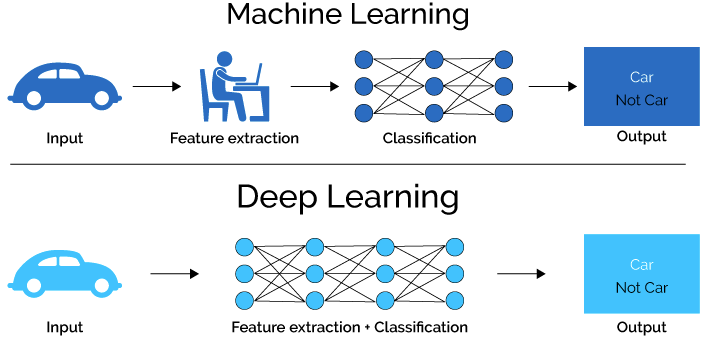
\includegraphics[scale = 0.25]{pics/MLvsDL.png}
\end{figure}

\begin{itemize}
   \item El Aprendizaje Profundo proporciona resultados de última generación en la mayoría de las tareas de PNL.
   \item Grandes cantidades de datos de entrenamiento y máquinas GPU

 multicore más rápidas son clave en el éxito del aprendizaje profundo.
   \item Las \textbf{redes neuronales} y las \textbf{incrustaciones de palabras} desempeñan un papel fundamental en los modelos modernos de PNL.

\end{itemize}

\paragraph{Aprendizaje Profundo y Conceptos Lingüísticos}
\begin{itemize}
   \item Si los modelos de aprendizaje profundo pueden aprender representaciones automáticamente, ¿siguen siendo útiles los conceptos lingüísticos (por ejemplo, sintaxis, morfología)?
   \item Algunos defensores del aprendizaje profundo argumentan que estas propiedades lingüísticas inferidas y diseñadas manualmente no son necesarias, y que la red neuronal aprenderá estas representaciones intermedias (o equivalentes o mejores) por sí misma \cite{goldberg2016primer}.
   \item Aún no hay un consenso definitivo al respecto.
   \item Goldberg cree que muchos de estos conceptos lingüísticos pueden ser inferidos por la red por sí misma si se le proporciona suficiente cantidad de datos.
   \item Sin embargo, en muchos otros casos no disponemos de suficientes datos de entrenamiento para la tarea que nos interesa, y en estos casos proporcionar a la red los conceptos generales más explícitos puede ser muy valioso.
\end{itemize}

\section{Historia}

Los orígenes de PLN se remontan a los años 50 con el famoso test de Alan Turing: una máquina será considerada inteligente cuando sea capaz de conversar con una persona sin que esta pueda determinar si está hablando con una máquina o un ser humano. A lo largo de su historia la disciplina ha tenido tres grandes períodos: 1) el racionalismo, 2) el empirismo, y 3) el aprendizaje profundo [Deng y Liu, 2018] que describimos a continuación.

El racionalismo abarca desde 1950 a 1990, donde las soluciones consistían en diseñar reglas manuales para incorporar mecanismos de conocimiento y razonamiento. Un ejemplo emblemático es el agente de conversación (o chatbot) ELIZA desarrollado por Joseph Weizenbaum que simulaba  un psicoterapeuta rogeriano. Luego, a partir de la década de los 90s, el diseño de métodos estadísticos y de aprendizaje automático construidos sobre corpus llevan a PLN hacia un enfoque empirista. Las reglas ya no se construyen sino que se “aprenden” a partir de datos etiquetados.  Algunos modelos representativos de esta época son los filtros de spam basados en modelos lineales, las cadenas de Markov ocultas para la extracción de categorías sintácticas y los modelos probabilísticos de IBM para la traducción automática. Estos modelos se caracterizaban por ser poco profundos en su estructura de parámetros y por depender de características manualmente diseñadas para representar la entrada.

A partir del año 2010, las redes neuronales artificiales, que son una familia de modelos de aprendizaje automático, comienzan a mostrar resultados muy superiores en varias tareas emblemáticas de PLN [Collobert et al., 2011]. La idea de estos modelos es representar la entrada (el texto) con una jerarquía de parámetros (o capas) que permiten encontrar representaciones idóneas para la tarea en cuestión, proceso al cual se refiere como “aprendizaje profundo”. Estos modelos se caracterizan por tener muchos más parámetros que los modelos anteriores (superando la barrera del millón en algunos casos) y requerir grandes volúmenes de datos para su entrenamiento. Una gracia de estos modelos es que pueden ser pre-entrenados con texto no etiquetado como libros, Wikipedia, texto de redes sociales y de la Web para encontrar representaciones iniciales de palabras y oraciones (a lo que conocemos como word embeddings),  las cuales pueden ser posteriormente adaptadas para la tarea objetivo donde sí se tienen datos etiquetados (Proceso conocido como transfer learning). Aquí destacamos modelos como Word2Vec [Mikolov 2013], BERT  [Devlin 2018] y GPT-3  [Brown 2020].

Este tipo de modelos ha ido perfeccionándose en los últimos años, llegando a obtener resultados cada vez mejores para casi todos los problemas del área [NLPProgress]. Sin embargo, este progreso no ha sido libre de controversias. El  aumento exponencial en la cantidad de parámetros de cada nuevo modelo respecto a su predecesor, hace que los recursos computacionales y energéticos necesarios para construirlos sólo estén al alcance de unos pocos. Además, varios estudios han mostrado que estos modelos aprenden y reproducen los sesgos y prejuicios (ej: género, religión, racial) presentes en los textos a partir de los cuales se entrenan. Sin ir más lejos, la investigadora  Timmnit Gebru fue despedida de Google  cuando se le negó el permiso para publicar un artículo que ponía de manifiesto estos problemas [Bender 2021].


El progreso de la PNL se puede dividir en tres oleadas principales: 1) racionalismo, 2) empirismo y 3) aprendizaje profundo \cite{deng2018deep}.
\begin{itemize}
   \item [1950 - 1990] Racionalismo: se enfocaba en diseñar reglas hechas a mano para incorporar conocimiento y mecanismos de razonamiento en sistemas de PNL inteligentes (por ejemplo, ELIZA para simular a un psicoterapeuta Rogeriano, MARGIE para estructurar información del mundo real en ontologías de conceptos).
   \item [1991 - 2009] Empirismo: se caracteriza por la explotación de corpora de datos y modelos de aprendizaje automático y estadísticos (superficiales) (por ejemplo, Naive Bayes, HMMs, modelos de traducción IBM).
   \item [2010 - ] Aprendizaje Profundo: la ingeniería de características (considerada como un cuello de botella) se reemplaza con el aprendizaje de representaciones y/o redes neuronales profundas (por ejemplo, \url{https://www.deepl.com/translator}). Un artículo muy influyente en esta revolución: \cite{collobert2011natural}.
\end{itemize}

\footnotetext{Las fechas son aproximadas.}

\section{Conclusiones}


En este capítulo, hemos explorado el desafío de entender y producir lenguaje utilizando computadoras. El aprendizaje automático supervisado es una de las principales técnicas utilizadas para abordar este desafío. Además, hemos discutido las propiedades desafiantes del lenguaje, como la discreción, la composicionalidad y la dispersión. Estos aspectos nos muestran la complejidad inherente al procesamiento del lenguaje natural y nos desafían a encontrar soluciones efectivas.




\chapter{Modelo de Espacio Vectorial y Recuperación de Información}
\label{cap_ir}

En este capítulo, exploraremos las primeras técnicas utilizadas para representar el lenguaje en forma vectorial. Para contextualizar esto, planteamos las siguientes preguntas:

\begin{itemize}
   \item ¿Cómo recuperan los motores de búsqueda, como Duckduckgo o Google, los documentos relevantes a partir de una consulta dada?
   \item ¿Cómo pueden las empresas procesar las reclamaciones dejadas por sus usuarios en sus portales web?
\end{itemize}

Estas preguntas suelen abordarse desde dos disciplinas relacionadas:

\begin{itemize}
   \item \emph{Recuperación de Información}: ciencia que se ocupa de buscar información en colecciones de documentos.
   \item \emph{Minería de Texto}: extracción automática de conocimiento a partir de texto.
\end{itemize}

Ambas disciplinas están estrechamente vinculadas al PLN, y las fronteras entre estos campos no siempre están claras.

\section{Tokens y Tipos}

El primer paso en el procesamiento de texto es, generalmente, la \textbf{tokenización}, que consiste en dividir una oración o documento en fragmentos llamados \emph{tokens}. A menudo, se acompañan otras transformaciones adicionales, como la eliminación de caracteres especiales (por ejemplo, puntuación), la conversión de todo el texto a minúsculas y otras operaciones descritas en este capítulo.

\paragraph{Ejemplo}

Entrada: ``Me gustan los lenguajes humanos y los lenguajes de programación.''

Tokens: [Me] [gustan] [los] [lenguajes] [humanos] [y] [los] [lenguajes] [de] [programación]

\subsection{Tipos}

Un \emph{tipo} es una clase de \emph{token} que contiene una secuencia única de caracteres. Los tipos se obtienen identificando los tokens únicos dentro del documento.

Por ejemplo, para la oración anterior, los tipos serían: [Me] [gustan] [los] [lenguajes] [humanos] [y] [de] [programación]. Observemos que el token \emph{lenguajes} se incluye solo una vez en la lista de tipos.

\paragraph{Extracción de Vocabulario}

Un \emph{término} es un \emph{tipo} normalizado. La normalización implica la creación de clases de equivalencia para diferentes \emph{tipos}, por ejemplo, cuando tratamos de manera indistinta dos tokens que difieren solo en el uso de mayúsculas (hombre y Hombre). El vocabulario $V$ es el conjunto de términos (tokens únicos normalizados) dentro de una colección de documentos o corpus $D$.

\section{Eliminación de Stopwords}

Con el fin de reducir el tamaño del vocabulario y eliminar términos que no aportan mucha información, se eliminan los términos que ocurren con alta frecuencia en el corpus (o colección de documentos). Estos términos se llaman \emph{stopwords} e incluyen artículos, pronombres, preposiciones y conjunciones.

Ejemplo de stopwords: [un, una, y, cualquier, no, el, en].

Es importante tener en cuenta que la eliminación de stopwords puede ser inconveniente en muchas tareas de procesamiento del lenguaje natural. Por ejemplo, en la oración ``No me gusta la pizza'', al eliminar la negación, se pierde información valiosa sobre el sentimiento de la oración.

\section{Stemming}

Es un proceso de normalización de términos en el cual los términos se transforman a su raíz con el objetivo de reducir el tamaño del vocabulario. Se lleva a cabo aplicando reglas de reducción de palabras. La Tabla~\ref{tab:porter} muestra  algunas reglas del algortimo de Porter para el inglés con ejemplos de aplicación:

\begin{table}[h]
\centering
\begin{tabular}{|l|l|}
\hline
Regla & Ejemplo \\
\hline
SSES $\rightarrow$ SS & caresses $\rightarrow$ caress \\
IES $\rightarrow$ I & ponies $\rightarrow$ poni \\
SS $\rightarrow$ SS & caress $\rightarrow$ caress \\
S $\rightarrow$ & cats $\rightarrow$ cat \\
\hline
\end{tabular}
\caption{Ejemplos del Algortimo de Porter}
\label{tab:porter}
\end{table}

A continuación se muestra ejemplo usando el método de stemming Snowball para español para el lenguaje \textbf{python} usando la biblioteca \textbf{nltk}.

\begin{verbatim}
from nltk import word_tokenize
from nltk.stem import SnowballStemmer
stemmer = SnowballStemmer('spanish')
texto = 'Me gustan los lenguajes humanos y los lenguajes de programación'
def stem_sentence(text):
    return ' '.join([stemmer.stem(i) for i in word_tokenize(text)])    
print(stem_sentence(texto))
>>
me gust los lenguaj human y los lenguaj de program
\end{verbatim}



\section{Lematización}
Otra estrategia de normalización de términos. También transforma las palabras en sus raíces.  Realiza un análisis morfológico utilizando diccionarios de referencia (tablas de búsqueda) para crear clases de equivalencia entre \emph{tipos}. Por ejemplo, para el token \emph{yendo}, una regla de stemming devolvería el término \emph{yend}, mientras que a través de la lematización obtendríamos el término \emph{ir}.

Veamos a continuación el resultado de aplicar lematización a la misma oración anterior con la biblioteca \textbf{spacy}:

\begin{verbatim}
# python -m spacy download es_core_news_sm
import spacy
nlp = spacy.load('es_core_news_sm')

def lemmatizer(text):  
  doc = nlp(text)
  return ' '.join([word.lemma_ for word in doc])

print(lemmatizer(texto))
>>
yo gustar el lenguaje humano y el lenguaje de programación
\end{verbatim}



\section{Ley de Zipf}
La Ley de Zipf, propuesta por George Kingsley Zipf en \cite{zipf1935}, es una ley empírica que describe la frecuencia de los términos en una colección de documentos (corpus). Según esta ley, la frecuencia $f$ de un término en un corpus es inversamente proporcional a su posición $r$ en una tabla de frecuencias ordenada:

\begin{equation}
f = \frac{cf}{r^{\beta}}
\end{equation}

Aquí, $cf$ es una constante dependiente de la colección y $\beta > 0$ es un factor de decaimiento. Cuando $\beta = 1$, la frecuencia sigue exactamente la Ley de Zipf, de lo contrario, sigue una distribución similar a la de Zipf. Esta ley nos indica que algunas palabras se utilizan con mucha más frecuencia que otras en un corpus. La Ley de Zipf se clasifica como una distribución de ley de potencia, que es un tipo de distribución de cola larga.

\begin{figure}[h!]
\centering
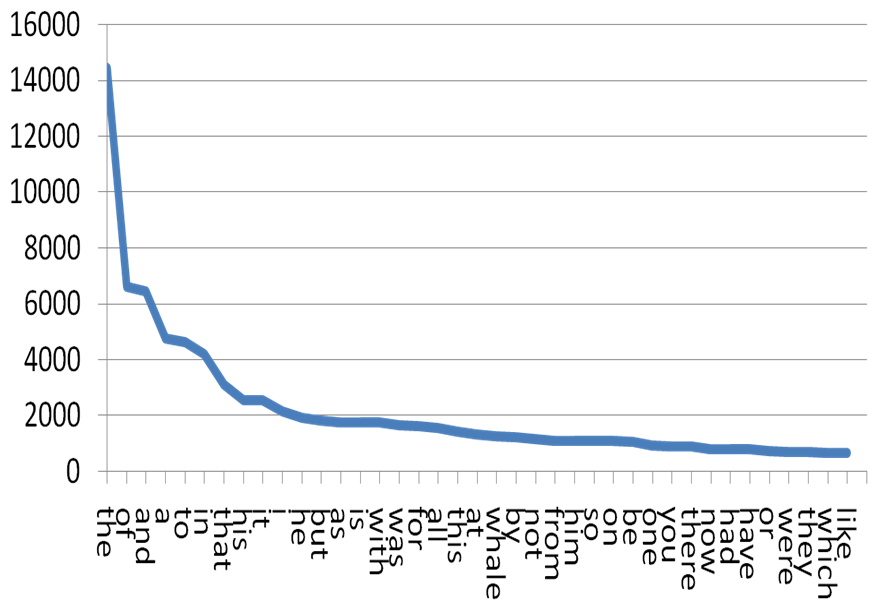
\includegraphics[scale=0.5]{pics/zipf1.png}
\caption{Ley de Zipf.}
\end{figure}

Cuando trazamos un gráfico en escala logarítmica ($log$-$log$), se obtiene una línea recta con una pendiente de $-\beta$. Esta relación logarítmica es útil para identificar las palabras más frecuentes en un corpus y construir una lista de stopwords.


\section{Listas de posteo y el índice invertido}
Sea $D$ una colección de documentos y $V$ el vocabulario de todos los términos extraídos de la colección:

\begin{itemize}
\item La lista de posteo de un término es la lista de todos los documentos donde el término aparece al menos una vez. Los documentos se identifican por sus identificadores.
\item Un índice invertido es una estructura de datos tipo diccionario que mapea los términos $t_{i} \in V$ con sus listas de posteo correspondientes.
\begin{displaymath}
<\text{término}> \rightarrow <\text{idDocumento}>^*
\end{displaymath}
\end{itemize}

\begin{figure}[h!]
\centering
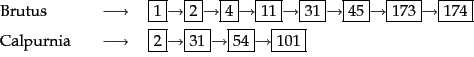
\includegraphics[scale=0.6]{pics/invFile.png}
\caption{Índice invertido}
\end{figure}

\section{Motores de búsqueda web}

Un motor de búsqueda es un sistema de recuperación de información diseñado para buscar información en la web (satisfacer necesidades de información) \cite{manning2008}. Sus componentes básicos son:

\begin{itemize}
\item Crawler: un robot que navega por la web según una estrategia definida. Por lo general, comienza navegando por un conjunto de sitios web iniciales (semillas) y continúa navegando a través de sus enlaces.
\item Indexador: se encarga de mantener un índice invertido con el contenido de las páginas recorridas por el rastreador.
\item Procesador de consultas: se encarga de procesar las consultas de los usuarios y buscar en el índice los documentos más relevantes para una consulta.
\item Función de ranking: la función utilizada por el procesador de consultas para ordenar los documentos indexados en la colección por relevancia según una consulta.
\item Interfaz de usuario: recibe la consulta como entrada y devuelve los documentos ordenados por relevancia.
\end{itemize}

\begin{figure}[h!]
\centering
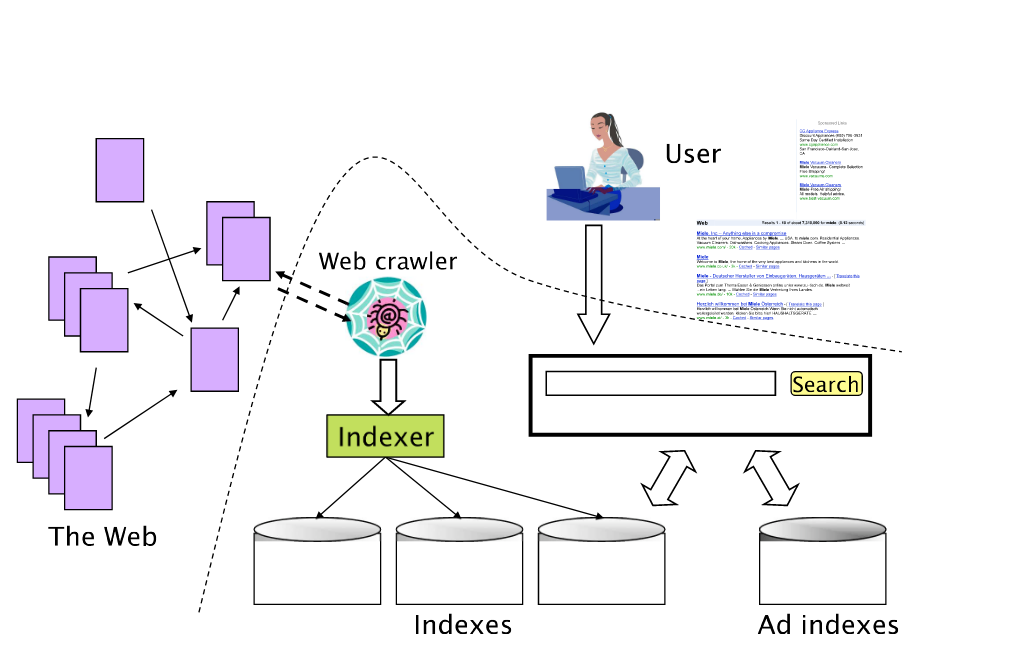
\includegraphics[scale=0.25]{pics/searchengine.png}
\caption{Los diversos componentes de un motor de búsqueda web \cite{manning2008}.}
\end{figure}


\section{El modelo de espacio vectorial}
Para clasificar consultas o medir la similitud entre dos documentos, necesitamos una métrica de similitud. Los documentos pueden ser \textit{representados} como vectores de términos, donde cada término es una dimensión del vector \cite{salton1975vector}. Documentos con diferentes palabras y longitudes residirán en el mismo espacio vectorial. Este tipo de representaciones se llaman \emph{Bolsa-de-palabras} (Bag of Words). En las representaciones de bolsa de palabras, se pierde el orden de las palabras y la estructura lingüística de una oración.

El valor de cada dimensión es un peso que representa la relevancia del término $t_{i}$ en el documento $d$.
\begin{equation}
d_{j} \rightarrow \overrightarrow{d_{j}}=(w(t_{1},d_{j}),...,w(t_{|V|},d_{j}))
\end{equation}

¿Cómo podemos modelar la información que aporta un término a un documento? Necesitamos formas de ponderar eso.

\subsection{Frecuencia de Término - Frecuencia Inversa de Documento}
Sea $tf_{i,j}$ la frecuencia del término $t_{i}$ en el documento $d_{j}$.  Un término que ocurre 10 veces debería proporcionar más información que uno que ocurre solo una vez. ¿Qué ocurre cuando tenemos documentos que son mucho más largos que otros? Podemos normalizar dividiendo por la frecuencia máxima del término en el documento.
\begin{displaymath}
ntf_{i,j}=\frac{tf_{i,j}}{\max_i (tf_{i,j})}
\end{displaymath}

Ahora podemos preguntarnos ¿un término que ocurre en muy pocos documentos proporciona más o menos información que uno que ocurre varias veces? Por ejemplo, el documento \emph{El respetado alcalde de Pelotillehue}. El término \emph{Pelotillehue} ocurre en menos documentos que el término \emph{alcalde}, por lo que debería ser más descriptivo.

Sea $N$ el número de documentos en la colección y $n_{i}$ el número de documentos que contienen el término $t_{i}$, definimos la frecuencia inversa de documento ($idf$) de $t_{i}$ de la siguiente manera:
\begin{displaymath}
idf_{t_{i}}= \log_{10}\left(\frac{N}{n_{i}}\right)
\end{displaymath}

Un término que aparece en todos los documentos tendría $idf=0$, y uno que aparece en el $10\%$ de los documentos tendría $idf=1$. El modelo $tf$-$idf$ combina los valores de $tf$ e $idf$, y resulta en los siguientes pesos $w$ para un término en un documento:
\begin{displaymath}
w(t_{i},d_{j})=tf_{i}\times \log_{10}\left(\frac{N}{n_{i}}\right)
\end{displaymath}

Las consultas de los motores de búsqueda también pueden ser modeladas como vectores. Sin embargo, en promedio, las consultas suelen tener entre 2 y 3 términos. Para evitar tener demasiadas dimensiones nulas, los vectores de consulta pueden suavizarse de la siguiente manera:
\begin{displaymath}
w(t_{i},d_{j})=(0.5+0.5\times tf_{i,j})\log_{10}\left(\frac{N}{n_{i}}\right)
\end{displaymath}

\subsection{Similitud entre vectores}
Representar consultas y documentos como vectores permite calcular su similitud. Un enfoque podría ser utilizar la distancia euclidiana. El enfoque común es calcular el coseno del ángulo entre los dos vectores. Si ambos documentos son iguales, el ángulo sería $0$ y su coseno sería $1$. Por otro lado, si son ortogonales, el coseno es $0$. La similitud del coseno se calcula de la siguiente manera:
\begin{displaymath}
\text{similitud del coseno}(\vec{d}{1},\vec{d}{2})= \frac{\vec{d}{1}\cdot \vec{d}{2}}{|\vec{d}{1}|\times|\vec{d}{2}|} = \frac{\sum_{i=1}^{|V|}(w(t_{i},d_{1})\times w(t_{i},d_{2}))}{\sqrt{\sum_{i=1}^{|V|} w(t_{i},d_{1})^2}\times \sqrt{\sum_{i=1}^{|V|} w(t_{i},d_{2})^2}}
\end{displaymath}

Esto se llama incorrectamente ``distancia del coseno''. En realidad, es una métrica de similitud pues entre más cerca dos vectores mayor es el valor asociado. Nótese que la similitud del coseno normaliza los vectores por su norma euclidiana $||\vec{d}||_{2}$.

\begin{figure}[h!]
\centering
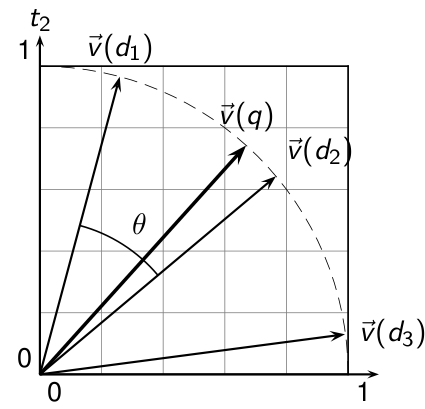
\includegraphics[scale=0.5]{pics/cos.png}
\caption{Similitud del coseno.}
\end{figure}

\paragraph{Ejercicio}
\begin{itemize}
\item Supongamos que tenemos $3$ documentos formados a partir de las siguientes secuencias de términos: \
$d_{1}\rightarrow t_{4}t_{3}t_{1}t_{4}$ \
$d_{2}\rightarrow t_{5}t_{4}t_{2}t_{3}t_{5}$ \
$d_{3}\rightarrow t_{2}t_{1}t_{4}t_{4}$ \
\item Construya una matriz término-documento de dimensiones $5\times3$ utilizando pesos simples de $tf$-$idf$ (sin normalización).
\item Recomendamos que primero construyas una lista con el número de documentos en los que aparece cada término (útil para calcular los valores de $idf$).
\item Luego, calcula los valores de $idf$ para cada término.
\item Rellena las celdas de la matriz con los valores de $tf$-$idf$.
\item ¿Cuál es el documento más cercano a $d_{1}$?
\end{itemize}

Resultado:
 \begin{table}[h]
 \centering
\begin{tabular}{|l|r|r|r|}
\hline
 & \multicolumn{1}{l|}{d1} & \multicolumn{1}{l|}{d2} & \multicolumn{1}{l|}{d3} \\ \hline
t1 & 0.176 & 0.000 & 0.176 \\ \hline
t2 & 0.000 & 0.176 & 0.176 \\ \hline
t3 & 0.176 & 0.176 & 0.000 \\ \hline
t4 & 0.000 & 0.000 & 0.000 \\ \hline
t5 & 0.000 & 0.954 & 0.000 \\ \hline
\end{tabular}
\caption{Matriz tf-idf}
\end{table}
\section{Clustering de Documentos}

¿Cómo podemos agrupar (o clusterizar) documentos que sean similares entre sí? El clustering es el proceso de agrupar documentos que comparten similitudes. Cada grupo de documentos se denomina \emph{cluster}. En el clustering, buscamos identificar grupos de documentos donde la similitud entre los documentos del mismo grupo se maximice, mientras que la similitud entre los documentos de diferentes grupos se minimice.

\begin{figure}[h!]
\centering
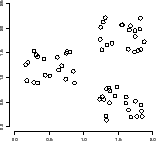
\includegraphics[scale=0.6]{pics/cluster.png}
\caption{Conjunto de documentos donde los grupos se pueden identificar claramente.}
\end{figure}

El clustering de documentos permite identificar tópicos en un corpus y reducir el espacio de búsqueda en un motor de búsqueda. Por ejemplo, el índice invertido se organiza según los grupos. El algoritmo K-means es una técnica de clustering simple que toma como parámetro el número de grupos, $k$.

El algoritmo se basa en la noción de \emph{centroides}, que son los vectores promedio de los documentos pertenecientes al mismo grupo. Por ejemplo, dado un conjunto de vectores bidimensionales $S = \{(3,6), (1,2), (5,1)\}$, el centroide de $S$ sería $(3,3)$, calculado como $(3+1+5)/3$ y $(6+2+1)/3$.

El algoritmo K-means comienza seleccionando $k$ centroides de manera aleatoria. Luego, calcula la similitud entre cada documento y cada centroide, asignando cada documento al centroide más cercano, formando así un grupo. Los centroides se recalculan de acuerdo con los documentos asignados a ellos. Este proceso se repite hasta que se cumple un criterio de convergencia, como se ilustra en el Algoritmo~\ref{algo:kmeans}.

\begin{algorithm}[H]
\SetKwInOut{Input}{Input}
\SetKwInOut{Output}{Output}
    \Input{Datos vectoriales $\vec{x}_1, \ldots, \vec{x}_N$ y el número de clusters $K$}
    \Output{centroides de clusters $\vec{\mu}_1, \ldots, \vec{\mu}_K$}
    $(\vec{s}_1, \vec{s}_2, \ldots, \vec{s}_K) \leftarrow$ SELECT\_RANDOM\_SEEDS($\vec{x}_1, \ldots, \vec{x}_N$, $K$)\;
    \For{$k \leftarrow 1$ \KwTo $K$}{
        $\vec{\mu}_k \leftarrow \vec{s}_k$\;
    }
    \While{no se cumpla el criterio de parada}{
        \For{$k \leftarrow 1$ \KwTo $K$}{
            $\omega_k \leftarrow \{\}$\;
        }
        \For{$n \leftarrow 1$ \KwTo $N$}{
            $j \leftarrow \arg\max_{j'} $coseno$(\vec{\mu}_{j'}, \vec{x}_n)$\;
            $\omega_j \leftarrow \omega_j \cup \{\vec{x}_n\}$\;
        }
        \For{$k \leftarrow 1$ \KwTo $K$}{
            $\vec{\mu}_k \leftarrow \frac{1}{{|\omega_k|}} \sum_{\vec{x} \in \omega_k} \vec{x}´$\;
        }
    }
    \Return{$\{\vec{\mu}_1, \ldots, \vec{\mu}_K\}$}\;
    \caption{K-Means}\label{algo:kmeans}
\end{algorithm}

\section{Conclusiones y Conceptos Adicionales}

En este capítulo, hemos explorado la representación de documentos como vectores para calcular similitudes entre ellos. Los vectores de ``bolsa-de-palabras'' son una forma común de representar documentos, pero tienen limitaciones ya que carecen de estructura lingüística y pueden ser de alta dimensionalidad y dispersos.

Una alternativa para capturar expresiones de múltiples palabras es utilizar n-gramas de palabras, que son secuencias contiguas de $n$ palabras. Por ejemplo, representar ``New York'' como ``new\_york'' nos permite capturar la relación entre esas dos palabras en lugar de tratarlas como entidades separadas.

Es importante señalar que los sistemas modernos de recuperación de información van más allá de la similitud de vectores. Utilizan algoritmos como PageRank \cite{page1998pagerank} para determinar la relevancia de un sitio web basándose en los enlaces que lo apuntan. También emplean técnicas de aprendizaje automático que utilizan registros de consultas anteriores para mejorar el ranking de resultados. Además, el uso de grafos de conocimiento enriquece aún más los resultados al proporcionar información estructurada y relaciones entre entidades.

Es importante destacar que disciplinas como la recuperación de información y la minería de textos se centran menos en la estructura lingüística que PLN y más en producir algoritmos rápidos y escalables para procesar grandes volúmenes de texto.



\chapter{Modelos de Lenguaje Probabilísticos}
\label{cap_plm}

En esta sección introducimos el concepto de ``modelo de lenguaje''. Un enfoque para asignar probabilidades a las oraciones que, como veremos a lo largo del apunte, desempeñará un papel fundamental en los enfoques modernos de PLN.

\section{El Problema del Modelado del Lenguaje}
Supongamos que tenemos un corpus de documentos $\mathcal{C}$, del cual extraemos su vocabulario (finito) a partir de la tokenización de sus documentos, $\mathcal{V} = \{$el, un, hombre, telescopio, Zamorano, dos, fan, vio, jugar, para, Real, Madrid, Zamorano, . . .$\}$.

Podemos formar a partir de este vocabulario un conjunto infinito de oraciones si dejamos que éstas sean de largo variable, $\mathcal{V}^*$. 

\begin{example}
Algunas oraciones que podríamos formar:
\begin{itemize}
\item el STOP
\item un STOP
\item el fan STOP
\item el fan vio a Zamorano STOP
\item el fan vio vio STOP
\item el fan vio a Zamorano jugar por el Real Madrid STOP
\end{itemize}

Donde STOP es un símbolo especial que indica el final de una oración.  
\end{example}

\begin{definition}
Un modelo de lenguaje es una distribución de probabilidad $p$ sobre todas las oraciones que se pueden formar a partir de un vocabulario finito. Entonces, la probabilidad de cada oración debe ser mayor o igual que cero, y la suma de las probabilidades de todas las oraciones posibles debe ser uno: 
\begin{align*}
\sum_{x\in V^*} p(x) &= 1 \\
p(x) &\geq 0 \quad \text{para todo } x \in V^*
\end{align*}
\end{definition}


\begin{example}
A continuación mostramos ejemplos de probabilidades asignadas por un modelo de lenguaje imaginario a algunas oraciones:
\begin{align*}
p(\text{el STOP}) &= 10^{-12} \\
p(\text{el fan STOP}) &= 10^{-8} \\
p(\text{el fan vio a Zamorano STOP}) &= 2 \times 10^{-8} \\
p(\text{el fan vio vio STOP}) &= 10^{-15} \\
\ldots \\
p(\text{el fan vio a Zamorano jugar por el Real Madrid STOP}) &= 2 \times 10^{-9}
\end{align*}
\end{example}



Lo que esperamos del modelo es que le asigne una probabilidad más alta a las oraciones fluidas (aquellas que tienen sentido y son gramaticalmente correctas) de las que no. También esperamos poder estimar esta función de probabilidad a partir del texto (corpus).

A nivel general, el modelo de lenguaje ayuda a los modelos de generación de texto a distinguir entre buenas y malas oraciones.


\subsection{¿Por qué querríamos hacer esto?}

La motivación original de estos modelos se origina en el problema de reconocimiento del habla o de transcripción automática para ayudar a estos sistemas a discernir entre disitntas oraciones compatibles con la señal acústica.  Consideremos las siguientes dos oraciones en inglés:
\begin{enumerate}
 \item ``recognize speech''  (reconocer el habla)
 \item ``wreck a nice beach'' (arruinar una playa bonita).
\end{enumerate}

Estas dos oraciones suenan muy similares al ser pronunciadas (tienen casi la misma señal acústica), lo que dificulta que los sistemas automáticos de reconocimiento del habla las transcriban con precisión. Cuando el sistema de reconocimiento del habla analiza la entrada de audio e intenta transcribirlo, tiene en cuenta las probabilidades del modelo de lenguaje para determinar la interpretación más probable.
El modelo de lenguaje favorecería $p$(``recognize speech'') sobre $p$(``wreck a nice beach'').
Esto se debe a que la primera oración es más común y debería ocurrir con más frecuencia en el corpus de entrenamiento.

Al incorporar modelos de lenguaje, los sistemas de reconocimiento del habla pueden mejorar  la precisión al seleccionar la oración que se alinea mejor con los patrones lingüísticos y el contexto, incluso cuando se enfrentan a alternativas que suenan similar.

De hecho, los modelos de lenguaje son útiles en cualquier tarea de procesamiento del lenguaje natural que involucre la generación de lenguaje (por ejemplo, traducción automática, resumen, generación de resúmenes, chatbots,  reconocimiento óptico de caracteres y el reconocimiento de escritura a mano).

Además la noción de modelamiento probabilístico del lenguaje se utiliza en muchos modelos y tareas de PLN, por lo que las técnicas de estimación desarrolladas en este capítulo serán muy útiles para entender muchos problemas en PLN.


\section{Regla de la Cadena en Modelos de Lenguaje}

En el contexto de los modelos de lenguaje, se parte de la premisa de que cualquier oración $s$ puede ser vista como una secuencia de variables aleatorias $X_1, X_2, \ldots, X_n$. Cada una de estas variables aleatorias puede tomar valores de un conjunto finito $V$. Para simplificar, asumimos una longitud fija $n$ para la secuencia. Nuestro objetivo consiste en modelar la probabilidad conjunta $p(X_1 = x_1, X_2 = x_2, \ldots, X_n = x_n)$. Es importante notar que utilizamos letras mayúsculas para denotar las variables aleatorias ($X_1, X_2, \ldots, X_n$) y minúsculas para referirnos a instancias específicas de estas variables ($x_1, x_2, \ldots, x_n$), que representan elementos del vocabulario (por ejemplo, ``perro'', ``gato'', ``comida'').

Una forma común de representar secuencias de variables aleatorias es mediante la aplicación de la regla de la cadena de probabilidades que definimos a continuación.

Para un conjunto de variables aleatorias $X_1,\ldots, X_n$, la regla de la cadena de probabilidades nos permite expresar la función de probabilidad conjunta $p(X_1,X_2,\ldots, X_n)$ como un producto de $n$ probabilidades condicionales:

\begin{equation}\label{eq:cadena}
p(X_1,X_2,\ldots,X_n)=p(X_1)p(X_2|X_1)p(X_3|X_2,X_1)\ldots p(X_n|X_{n-1},\ldots,X_2,X_1).
\end{equation}

Por ejemplo, en el caso de $n=3$, la expresión se simplifica a:

\begin{displaymath}
p(X_1,X_2,X_3)=p(X_1)p(X_2|X_1)p(X_3|X_2,X_1).
\end{displaymath}

Al utilizar la definición de probabilidades condicionales, podemos expresar $p(X_2|X_1)$ como $p(X_1,X_2)/p(X_1)$ y $p(X_3|X_2,X_1)$ como $p(X_1,X_2,X_3)/p(X_1,X_2)$. Al sustituir estas expresiones en la cadena de productos, vemos que todas las expresiones de cancelan y finalmente obtenemos $p(X_1,X_2,X_3)$.     

La aplicación de la regla de la cadena en los modelos de lenguaje no impone ningún supuesto específico sobre el modelo en sí. Más bien, nos proporciona una forma alternativa de modelar la probabilidad de una oración. Sin embargo, la ventaja de utilizar la regla de la cadena es que nos permite aplicar supuestos y hacer simplificaciones en el modelo para facilitar su implementación y cálculo.

\section{Mirada Predictiva}
La regla de la cadena nos permite darle una interpretación predictiva a los modelos de lenguaje. Uno puede asumir que un modelo de lenguaje una vez entrenado (o construido) a partir de un corpus es capaz de entregar una distribución de probabilidad para todas las palabras a partir de un contexto específico. Supongamos que tenemos un contexto formado por una secuencia de palabras $c=X_{n-1},\ldots,X_1$ y queremos predecir la palabra más probable a partir de ese contexto. Uno podría evaluar la probabilidad condicional $p(X_n|X_{n-1},\ldots,X_1)$ o $p(X_n|c)$ para todas las palabras del vocabulario que puede tomar $X_n$ y escoger la más probable:

\begin{displaymath}
x_n = \operatorname{argmax}_{X_n \in \mathcal{V}} p(X_n | c)
\end{displaymath}


\begin{example}
Supongamos que el contexto es $c=$``Cristóbal Colón descubrió''. El modelo de lenguaje sería capaz de determinar:

\begin{align*}
p(X|\text{``descubrió'', Colón'', ``Cristóbal''}) \\
\forall X \in V, \quad \text{donde} \sum_{X\in V}p(X|c)=1 
\end{align*}

Por ejemplo:

 
\begin{align*}
p(\text{``América''}|\text{``descrubrió'', ``Colón'', ``Cristóbal''}) = 0.02 \\
p(\text{``Europa''}|\text{``descrubrió'', ``Colón'', ``Cristóbal''}) = 0.01 \\
p(\text{``Chile''}|\text{``descrubrió'', ``Colón'', ``Cristóbal''}) = 0.001\\
p(\text{``camello''}|\text{``descrubrió'', ``Colón'', ``Cristóbal''}) = 0.00001 \\
\ldots
\end{align*}

Entonces, nuestro modelo de lenguaje predeciría $X=$``América'' como la palabra siguiente más probable.  
\end{example}

En el ejemplo anterior esperamos que un buen modelo de lenguaje asigne una probabilidad mayor a $X=$``América'' que al resto de las opciones. Para realizar estas predicciones, el modelo de lenguaje necesita capturar las reglas sintácticas y semánticas del lenguaje, así como tener un amplio conocimiento del mundo. 


Otra propiedad relevante, que se abordará en el Capítulo~\ref{cap_llm} sobre grandes modelos de lenguaje, es que se puede codificar prácticamente cualquier tarea de PLN como una instrucción dentro del contexto de un modelo de lenguaje. Por ejemplo, se podría utilizar la instrucción ``traduce el siguiente texto de inglés a español: I like dogs'', para luego esperar que el modelo de lenguaje sea capaz de realizar la traducción correcta.

\section{Mirada Generativa}

Los modelos de lenguaje aprendidos a partir de un corpus de texto no solo tienen una capacidad predictiva, sino que también tienen una capacidad generativa. Estos modelos pueden utilizarse para generar oraciones nuevas muestreando secuencialmente a partir de las probabilidades condicionales estimadas.

El proceso generativo implica tomar una palabra inicial y, a medida que avanzamos en la generación, seleccionar sucesivas palabras basadas en las probabilidades condicionales proporcionadas por el modelo de lenguaje. Es similar a extraer bolas (palabras) de una urna, donde los tamaños de las bolas están en proporción a sus frecuencias relativas, que son determinadas por el modelo de lenguaje. Cada vez que se selecciona una palabra, se utiliza como contexto para determinar la siguiente palabra, y así sucesivamente hasta que se haya generado una oración completa.

En este proceso generativo, hay diferentes enfoques que se pueden tomar. Uno de ellos es el muestreo estocástico, donde se elige una palabra de acuerdo con su probabilidad condicional dada por el modelo. Esto permite cierta variabilidad en la generación de oraciones, ya que las palabras menos probables también tienen la posibilidad de ser seleccionadas. Por otro lado, también se puede optar por seleccionar la palabra más probable en cada paso, lo que equivale a predecir la siguiente palabra basándose únicamente en la información disponible hasta ese momento. 


\section{Un Método Ingenuo}
Un método muy ingenuo para estimar la probabilidad de una oración es contar todas las apariciones de  oraciones idénticas a esta en los datos de entrenamiento y dividirlo por el número total de oraciones de entrenamiento ($N$).

Más formalmente, sea mi oración $s=x_1, x_2, \ldots, x_n$, y $c(x_1, x_2, \ldots, x_n)$  el número de veces que ocurre la oración en el corpus de entrenamiento, el modelo de lenguaje ingenuo computa la probabilidad de la siguiente manera: \begin{displaymath}
p(x_1,x_2,\cdots,x_n)=\frac{c(x_1,x_2 \dots,x_n)}{N}
\end{displaymath}

El problema de este enfoque, es que el número de posibles oraciones crece de manera exponencial con su cantidad de palabras y el tamaño del vocabulario. Entonces se vuelve cada vez más improbable que una oración específica haya ocurrido en los datos de entrenamiento. Esto es una consecuencia de la propiedad de \textbf{dispersión} del lenguaje planteada en el Capítulo~\ref{cap_intro}.

En consecuencia, muchas oraciones tendrán una probabilidad cero según el modelo ingenuo, lo que lleva a una mala generalización.

\section{Procesos de Markov}


Un proceso de Markov de primer orden asume que la probabilidad de que una variable aleatoria tome un valor depende únicamente del valor inmediatamente anterior en la secuencia. En el contexto del modelado del lenguaje, esto significa que la probabilidad de una palabra en una oración depende solo de la palabra anterior. Si aplicamos este supuesto a la regla de cadena de probabilidades, la probabilidad conjunta de una secuencia de palabras se simplifica en una multiplicación de probabilidades condicionales de las palabras sucesivas dado su palabra predecesora inmediata:

\begin{equation}
p(X_i = x_i|X_1 = x_1, \ldots, X_{i-1} = x_{i-1}) = p(X_i = x_i|X_{i-1} = x_{i-1})
\end{equation}




Un proceso de Markov de segundo orden amplía la suposición de Markov de primer orden y considera el valor de dos variables anteriores en la secuencia. En el modelado del lenguaje, esto significa que la probabilidad de una palabra en una oración depende de las dos palabras anteriores. La probabilidad conjunta de una secuencia de palabras se calcula multiplicando las probabilidades condicionales de las palabras sucesivas dado sus dos palabras predecesoras:

\begin{equation}
p(X_i = x_i|X_1 = x_1, \ldots, X_{i-2} = x_{i-2}, X_{i-1} = x_{i-1}) = p(X_i = x_i|X_{i-2} = x_{i-2}, X_{i-1} = x_{i-1})
\end{equation}


\subsection{Modelado de secuencias de longitud variable}

Si queremos modelar secuencias de longitud variable, podemos considerar que la longitud de la secuencia, $n$, también es una variable aleatoria. Una forma simple de abordar esto es siempre definir $X_n = \text{STOP}$, donde ``STOP'' es un símbolo especial que marca el final de la secuencia. Luego, podemos usar un proceso de Markov como antes para modelar la probabilidad conjunta de las palabras en la secuencia:

\[
p(X_1 = x_1, X_2 = x_2, \ldots, X_n = x_n) = \prod_{i=1}^{n} p(X_i = x_i|X_{i-2} = x_{i-2}, X_{i-1} = x_{i-1})
\]

Aquí, asumimos que $x_0 = x_{-1} = *$ por conveniencia, donde ``*'' es un símbolo especial de ``inicio'' de oración.

\section{Modelos de lenguaje de Trigramas}

Un n-grama es una secuencia contigua de $n$ palabras. Un modelo de lenguaje de trigrama (n-grama con $n=3$) acoge los supuestos de independencia del modelo de Markov de segundo orden que se discutió anteriormente. De esta forma permite expresar la probabilidad de una oración de la siguiente forma:
\begin{equation}
p(X_1,X_2,\ldots,X_n)=p(X_1)p(X_2|X_1)p(X_3|X_2,X_1)\ldots p(X_n|X_{n-1},X_{n-2}).
\end{equation}

Nótese que en vez de condicionar por todas las palabras anteriores como en la Ecuación~\ref{eq:cadena} aquí solo se condiciona por las dos palabras anteriores.


Los componentes que definen al modelo de lenguaje de trigrama se definen a continuación:

\begin{enumerate}
  \item Un vocabulario $V$, representado por un conjunto finito de palabras.
  \item Un parámetro escalar $q(w|u, v)$ para cada trigrama $u, v, w$, donde $w \in V \cup \{\text{STOP}\}$ y $u, v \in V \cup \{*\}$.
\end{enumerate}

Para cualquier oración $x_1 \ldots x_n$, donde $x_i \in V$ para $i = 1 \ldots (n-1)$ y $x_n = \text{STOP}$, la probabilidad de la oración según el modelo de lenguaje trigrama es:

\[
p(x_1 \ldots x_n) = \prod_{i=1}^{n} q(x_i|x_{i-2}, x_{i-1})
\]

Aquí, definimos $x_0 = x_{-1} = *$ como dos tokens especiales antes del inicio del oración para poder condicionar tanto la primera como la segunda palabra de una oración por sus dos palabras. A este tipo de transformaciones se les conoce en PLN como ``padding''.

Por ejemplo, para la oración ``el perro ladra STOP'', estimaríamos su probabilidad de la siguiente forma:
\[
p(\text{el perro ladra STOP}) = q(\text{el}|*, *) \times q(\text{perro}|*, \text{el}) \times q(\text{ladra}|\text{el}, \text{perro}) \times q(\text{STOP}|\text{perro}, \text{ladra})
\]

Ahora abordemos el problema de la estimación de los parámetros $q(w_i | w_{i-2}, w_{i-1})$ a partir de un corpus $\mathcal{C}$.

Una estimación natural es la ``estimación de máxima verosimilitud'' (MLE por sus siglas en inglés), donde se estiman los parámetros para maximizar la probabilidad de los datos de entrenamiento.

En el contexto de un modelo de trigrama, la estimación de cada parámetro proviene de distribuciones multinomiales, lo cual se traduce en el siguiente cálculo:

\[
q(w_i | w_{i-2}, w_{i-1}) = \frac{{\text{Count}(w_{i-2}, w_{i-1}, w_i)}}{{\text{Count}(w_{i-2}, w_{i-1})}}
\]

Esto requiere tokenizar el corpus de entrenamiento y guardar en una tabla los conteos de todos los trigramas (secuencias contiguas de 3 palabras) y bigramas (secuencias contiguas de dos palabras) encontrados.

Por ejemplo:
\[
q(\text{ladra} | \text{el, perro}) = \frac{{\text{Count}(\text{el, perro, ladra})}}{{\text{Count}(\text{el, perro})}}
\]




\section{Evaluación de un modelo de lenguaje: Perplejidad}

Un modelo de lenguaje efectivo se caracteriza por asignar probabilidades más altas a oraciones coherentes que a oraciones sin sentido. Para evaluar la calidad de un modelo de lenguaje, es esencial utilizar un corpus de prueba independiente diferente al corpus en el que fue entrenado. Esto nos permitirá verificar cómo generaliza el modelo a nuevas oraciones.  La evaluación cuantitativa de modelos de lenguaje nos permite comparar distintos tipos de modelos de lenguaje y seleccionar el modelo más apropiado.

Para evaluar un modelo de lenguaje utilizamos un corpus de prueba independiente, $\mathcal{C}_{\text{test}}$, que contiene $m$ oraciones: $s_1, s_2, s_3, ..., s_m$, y cuantificamos la probabilidad que el modelo asigna a estas oraciones. Para esto, calculamos la probabilidad total asignada por el modelo a las oraciones del corpus de prueba, lo cual se puede expresar más convenientemente mediante la probabilidad logarítmica\footnote{El logaritmo es una función monótona y permite llevar los productos a suma que evita problemas de underflow al trabajar con números pequeños.}:
\[
\log \left( \prod_{i=1}^{m} p(s_i) \right) = \sum_{i=1}^{m} \log p(s_i)
\]

La medida de evaluación estándar para modelos de lenguaje es la perplejidad (o perplexity), que se calcula de la siguiente manera:
\[
\text{Perplejidad} = 2^{-l} \quad \text{donde} \quad l = \frac{1}{M} \sum_{i=1}^{m} \log p(s_i)
\]

Donde $M$ es el número total de palabras en los datos de prueba.

La perplejidad es una métrica que favorece valores más bajos y tiene la propiedad de ser más fácil de interpretar que la probabilidad logarítmica, como se discutirá a continuación.


\subsection{Intuición sobre la perplejidad}

Supongamos que tenemos un vocabulario $V$, y $N = |V| + 1$, y un modelo de lenguaje ``uniforme'' que le asigna la misma probabilidad a todos los trigramas:
    \[
        q(w|u, v) = \frac{1}{N} \quad \text{para todo } w \in V \cup \{\text{STOP}\}, \text{ para todo } u, v \in V \cup \{*\}
    \]

La perplejidad de este modelo de lenguaje es $N$ tal como se demuestra a continuación.

Supongamos que tenemos $m$ oraciones de longitud $n$ en el corpus, y $M$ es la cantidad de tokens en el corpus, $M = m \cdot n$. Consideremos el logaritmo (base 2) de la probabilidad de una oración $s = w_1 w_2 \dots w_n$ bajo el modelo:
    \[
        \log p(s) = \log \prod_{i=1}^{n} q(w_i|w_{i-2}, w_{i-1}) = \sum_{i=1}^{n} \log q(w_i|w_{i-2}, w_{i-1})
    \]
Dado que cada parámetro $q(w_i|w_{i-2}, w_{i-1})$ es igual a $\frac{1}{N}$, tenemos:
    \[
        \log p(s) = \sum_{i=1}^{n} \log \frac{1}{N} = n \cdot \log \frac{1}{N} = -n \cdot \log N
    \]
    
    
    \[
        l =  \frac{1}{M} \sum_{i=1}^{m} \log p(s_i) = \frac{1}{M} \sum_{i=1}^{m} -n \cdot \log N  = \frac{1}{M} \cdot -m \cdot n \cdot \log N = - \log N 
    \]
    
            
Por lo tanto, la perplejidad está dada por:
    \[
        \text{Perplejidad} = 2^{-l} = 2^{-(- \log N)} = N
    \]

    
Esperamos entonces, que cualquier modelo de lenguaje que sea capaz de aprovechar la distribución de las palabaras (como un modelo de trigramas) tenga una perplejidad menor que el tamaño del vocabulario. En \cite{goodman2001bit}, donde $|V| = 50,000$, se presentan los siguientes resultados:

\begin{itemize}
        \item Modelo de trigramas: $p(x_1, \ldots, x_n) = \prod_{i=1}^n q(x_i | x_{i-2}, x_{i-1})$ \\
        Perplejidad = 74
        \item Modelo de bigramas: $p(x_1, \ldots, x_n) = \prod_{i=1}^n q(x_i | x_{i-1})$ \\
        Perplejidad = 137
        \item Modelo de unigramas: $p(x_1, \ldots, x_n) = \prod_{i=1}^n q(x_i)$ \\
        Perplejidad = 955
    \end{itemize}
    
Estos resultados muestran que la perplejidad disminuye a medida que aumentamos el nivel de contexto considerado en el modelo de lenguaje, lo que indica que los modelos con perplejidad más baja generalmente son más efectivos en la tarea de predicción del lenguaje. Sin embargo, como veremos a continuación, aumentar el tamaño del contexto no esta libre de problemas.   

\subsection{El trade-off entre sesgo y varianza}

Una limitación de los modelos de trigramas está relacionada con la dispersión del lenguaje, discutida en el Capítulo~\ref{cap_intro}. A grandes rasgos, si el tamaño del vocabulario es $N = |V|$, entonces el modelo tiene $N^3$ parámetros. Por ejemplo, si $N = 20,000$, habría $20,000^3 = 8 \times 10^{12}$ parámetros. Esta cantidad de parámetros es enorme y dificulta la estimación adecuada de todos ellos sin requerir un corpus de entrenamiento de tamaño enorme. Como resultado, puede surgir un problema de sobreajuste (overfitting) a los datos de entrenamiento. Por otro lado, modelos más simples, como un modelo de lenguaje de unigrama o de bigrama, no son capaces de modelar adecuadamente el contexto.

Este dilema es conocido en estadística y aprendizaje automático como el trade-off entre sesgo y varianza, que se refiere a la compensación entre la simplicidad del modelo y su capacidad para capturar la complejidad y variabilidad de los datos.

Los modelos más simples, como los modelos de n-gramas de orden inferior (unigramas, bigramas), tienen un sesgo más alto pero una varianza más baja. Estos modelos asumen independencia condicional entre las palabras y simplifican la estructura del lenguaje.

En contraste, los modelos más complejos, como modelos de n-gramas con $n>3$, tienen una varianza más alta pero un sesgo más bajo. Estos modelos pueden capturar relaciones más complejas entre las palabras, pero también son más propensos a sobreajustar los datos de entrenamiento y tener dificultades para generalizar a nuevas muestras.

Cuando se entrena un modelo de lenguaje con MLE, se maximiza la probabilidad de los datos de entrenamiento. Esto puede llevar a asignar probabilidades altas a secuencias específicas que aparecen en los datos de entrenamiento, incluso si esas secuencias son poco probables en la distribución real del lenguaje.

Como resultado, el modelo puede tener un rendimiento deficiente en datos de prueba que contienen secuencias diferentes a las del conjunto de entrenamiento. Esto se debe a que el modelo se ha sobreajustado a los datos de entrenamiento y ha capturado sus características específicas en lugar de aprender patrones más generales del lenguaje.

Para abordar el problema del sobreajuste en modelos de lenguaje, se utilizan diversas técnicas de regularización. Estas técnicas ayudan a controlar la varianza del modelo y mitigar el sobreajuste, permitiendo un mejor equilibrio entre el sesgo y la varianza y mejorando la generalización a nuevas muestras. A continuación, veremos dos técnicas de regularización para modelos de lenguaje: la interpolación lineal y los modelos de descuento.




\section{Interpolación Lineal}

La pricipal idea detrás de la técnica de interpolación lineal es combinar las distribuciones de probabilidad estimadas por modelos de n-gramas con las obtenidas a través de modelos de órdenes inferiores, como bigramas y unigramas. Esta estrategia ofrece la ventaja de incorporar información de n-gramas de órdenes más bajos, permitiendo abordar la indefinición de probabilidades en palabras no observadas durante el entrenamiento. Pues basta que una oración tenga un sólo trigrama no observado en entrenamiento para recibir una probabilidad de cero por el efecto multiplicativo de la regla de la cadena.

En el modelo interpolado, se ponderan linealmente tres modelos distintos:

\begin{enumerate}
    \item Modelo de trigramas: $q_{\text{ML}}(w_i | w_{i-2}, w_{i-1}) = \frac{{\text{Count}(w_{i-2}, w_{i-1}, w_i)}}{{\text{Count}(w_{i-2}, w_{i-1})}}$
    \item Modelo de bigramas: $q_{\text{ML}}(w_i | w_{i-1}) = \frac{{\text{Count}(w_{i-1}, w_i)}}{{\text{Count}(w_{i-1})}}$
    \item Modelo de unigramas: $q_{\text{ML}}(w_i) = \frac{{\text{Count}(w_i)}}{{\text{Count}(\# \text{tokens en el corpus})}}$.
\end{enumerate}

Cada parámetro $q(w_i | w_{i-2}, w_{i-1})$ se interpola de la siguiente manera:

\[
q(w_i | w_{i-2}, w_{i-1}) = \lambda_1 \cdot q_{\text{ML}}(w_i | w_{i-2}, w_{i-1}) + \lambda_2 \cdot q_{\text{ML}}(w_i | w_{i-1}) + \lambda_3 \cdot q_{\text{ML}}(w_i)
\]

Donde $\lambda_1$, $\lambda_2$, y $\lambda_3$ son hiper-parámetros que deben definirse manualmente y cumplir con las condiciones $\lambda_1 + \lambda_2 + \lambda_3 = 1$, y $\lambda_i \geq 0$ para todo $i$. Como podemos ver, con esta técnica abordamos el problema de indefinición de probabilidades en el modelo de trigramas, puesto que si se le quiere asignar probabilidad a un trigrama no observado durante entrenamiento, este no necesariamente indefine las probabilidades pues puede recurrir a las probabilidades de los bigramas y unigramas correspondientes.


Además, se puede demostrar que el modelo interpolado define adecuadamente una distribución de probabilidad (donde definimos $V' = V \cup \{\text{STOP}\}$):

\[
\begin{aligned}
    & \sum_{w \in V'} q(w | u, v) \\
    &= \sum_{w \in V'} [\lambda_1 \cdot q_{\text{ML}}(w | u, v) + \lambda_2 \cdot q_{\text{ML}}(w | v) + \lambda_3 \cdot q_{\text{ML}}(w)] \\
    &= \lambda_1 \sum_{w} q_{\text{ML}}(w | u, v) + \lambda_2 \sum_{w} q_{\text{ML}}(w | v) + \lambda_3 \sum_{w} q_{\text{ML}}(w) \\
    &= \lambda_1 + \lambda_2 + \lambda_3 = 1
\end{aligned}
\]

También es posible demostrar que $q(w | u, v) \geq 0$ para todas las palabras en $V'$, ya que es una suma ponderada de tres cantidades no negativas.



\subsection{Estimación de los Valores $\lambda$}
Para encontrar un valor adecuado de los hiper-parámetros $\lambda$ se suele reservar una parte del conjunto de entrenamiento como datos de \textit{validación}. Definimos $c'(w_1, w_2, w_3)$ como el número de veces que se observa el trigrama $(w_1, w_2, w_3)$ en el conjunto de validación. Elegimos $\lambda_1$, $\lambda_2$, $\lambda_3$ para maximizar:
    \[
    L(\lambda_1, \lambda_2, \lambda_3) = \sum_{w_1,w_2,w_3} c'(w_1, w_2, w_3) \log q(w_3 | w_1, w_2)
    \]
    sujetos a $\lambda_1 + \lambda_2 + \lambda_3 = 1$, y $\lambda_i \geq 0$ para todo $i$, donde
    \[
    q(w_i | w_{i-2}, w_{i-1}) = \lambda_1 \cdot q_{\text{ML}}(w_i | w_{i-2}, w_{i-1}) + \lambda_2 \cdot q_{\text{ML}}(w_i | w_{i-1}) + \lambda_3 \cdot q_{\text{ML}}(w_i)
    \]

Esto generalmente se hace buscando en una grilla de posibles valores de todos los hiper-parámetros. Nótese que maximizar $L(\lambda_1, \lambda_2, \lambda_3)$ es equivalente a minimizar la perplejidad en validación.


\section{Modelos de Descuento (Katz Back-Off)}

Los modelos de descuento representan una técnica alternativa a la interpolación con el propósito de mejorar la generalización del modelo de lenguaje a datos que difieren de los utilizados en el entrenamiento. Además, estos modelos ayudan a evitar la sobreestimación de conteos para n-gramas con baja frecuencia de aparición. La idea principal detrás de los modelos de descuento es redistribuir la probabilidad de los n-gramas observados hacia aquellos que no se han observado.

Para ilustrar estos modelos, consideremos un ejemplo utilizando los conteos de bigramas que comienzan con el unigrama ``la'' en un corpus, junto con sus estimaciones de máxima verosimilitud, que se presentan en la Tabla~\ref{tab:plm_ej}. Se puede notar que estas estimaciones tienden a sobrevalorar lo que se ha observado en el corpus y subestimar lo que no se ha observado.

\begin{table}[h]
    \centering
    \begin{tabular}{|l|l|l|}\hline
        \textbf{Frase} & \textbf{Conteo} & \textbf{$q_{\text{ML}}(w_i | w_{i-1})$} \\
        \hline
        la & 48 & \\
        la, gata & 15 & $15/48$ \\
        la, mujer & 11 & $11/48$ \\
        la, persona & 10 & $10/48$ \\
        la, plaza & 5 & $5/48$ \\
        la, actividad & 2 & $2/48$ \\
        la, tuerca & 1 & $1/48$ \\
        la, revista & 1 & $1/48$ \\
        la, tarde & 1 & $1/48$ \\
        la, ciudad & 1 & $1/48$ \\
        la, calle & 1 & $1/48$ \\ \hline
    \end{tabular}\caption{Ejemplo de conteos de bigramas}\label{tab:plm_ej}
\end{table}

Podemos definir los conteos ``descontados'' de la siguiente manera:

\[
\text{Conteo}^*(x) = \text{Conteo}(x) - \beta
\]

Donde $\beta$ es una constante que generalmente se encuentra entre 0 y 1, siendo un valor típico 0.5. Con $\beta=0.5$, los conteos se descuentan, es decir, se reduce la probabilidad de los datos observados, como se muestra en la Tabla~\ref{tab:plm_ej}.

\begin{table}[h]
    \centering
    \begin{tabular}{|l|l|l|l|}\hline
        \textbf{Frase} & \textbf{Conteo} & \textbf{Conteo}$\mathbf{^*(x)}$ & $\mathbf{q_{\text{BO}}(w_i | w_{i-1})}$ \\
        \hline
        la & 48 & & \\
        la, gata & 15 & 14.5 & $14.5/48$ \\
        la, mujer & 11 & 10.5 & $10.5/48$ \\
        la, persona & 10 & 9.5 & $9.5/48$ \\
        la, plaza & 5 & 4.5 & $4.5/48$ \\
        la, actividad & 2 & 1.5 & $1.5/48$ \\
        la, tuerca & 1 & 0.5 & $0.5/48$ \\
        la, revista & 1 & 0.5 & $0.5/48$ \\
        la, tarde & 1 & 0.5 & $0.5/48$ \\
        la, ciudad & 1 & 0.5 & $0.5/48$ \\
        la, calle & 1 & 0.5 & $0.5/48$ \\\hline
    \end{tabular}\caption{Ejemplo de conteos de bigramas con conteos descontados}\label{tab:plm_ej}
\end{table}

Las nuevas estimaciones se basan en los conteos descontados, y se introduce una ``masa de probabilidad faltante'' como se muestra a continuación:

\[
\alpha(w_{i-1}) = 1 - \sum_{w} \frac{\text{Conteo}^*(w_{i-1}, w)}{\text{Conteo}(w_{i-1})}
\]

Por ejemplo, en nuestro caso:

\[
\alpha(\text{la}) = 1 - \frac{14.5+10.5+9.5+4.5+1.5+0.5+0.5+0.5+0.5+0.5}{48} = 1-\frac{43}{48} = \frac{5}{48}
\]

La idea es redistribuir esta masa faltante entre todos los bigramas que comienzan con la palabra ``la'' y que no fueron observados en el corpus, como por ejemplo ``rana'', ``bailarina'' y ``puerta''.

En el modelo de Katz Back-Off de bigramas, se definen dos conjuntos: $A(w_{i-1})$ y $B(w_{i-1})$, como se detalla a continuación:

\[
A(w_{i-1}) = \{w : \text{Count}(w_{i-1}, w) > 0\}
\]

En nuestro ejemplo, $A(\text{la}) = \{$ gata, mujer, persona, plaza, actividad, tuerca, revista, tarde, ciudad, calle $\}$.

Por otro lado, $B(w_{i-1})$ se define como:

\[
B(w_{i-1}) = \{w : \text{Count}(w_{i-1}, w) = 0\}
\]

En nuestro ejemplo, $B(\text{la}) = \{$ rana, bailarina, puerta, $\dots$ $\}$.

Luego, la probabilidad condicional $q_{\text{BO}}(w_i | w_{i-1})$ se calcula de la siguiente manera: si la palabra $w_i$ está en el conjunto $A(w_{i-1})$, se utiliza una estimación basada en las frecuencias relativas de la secuencia $(w_{i-1}, w_i)$ dividida por la frecuencia de $w_{i-1}$. Si $w_i$ está en el conjunto $B(w_{i-1})$, se utiliza una estimación suavizada que combina la constante $\alpha(w_{i-1})$ y las probabilidades condicionales de máxima verosimilitud  de un modelo orden inferior (unigramas) $q_{\text{ML}}(w_i)$ de las palabras en el conjunto $B(w_{i-1})$. Esta última ponderación asegura que las probabilidades queden bien definidas.

\[
q_{\text{BO}}(w_i | w_{i-1}) =
\begin{cases}
    \frac{\text{Count}^*(w_{i-1}, w_i)}{\text{Count}(w_{i-1})} & \text{si } w_i \in A(w_{i-1}) \\
    \frac{\alpha(w_{i-1}) q_{\text{ML}}(w_i)}{\sum_{w \in B(w_{i-1})} q_{\text{ML}}(w)} & \text{si } w_i \in B(w_{i-1})
\end{cases}
\]

La constante $\alpha(w_{i-1})$ se calcula restando la suma de las frecuencias relativas de las palabras en $A(w_{i-1})$ de uno tal como se definió anteriormente.



Para extender este enfoque a trigramas, se definen conjuntos similares $A(w_{i-2}, w_{i-1})$ y $B(w_{i-2}, w_{i-1})$ para las secuencias de trigramas:

\[
A(w_{i-2}, w_{i-1}) = \{w : \text{Count}(w_{i-2}, w_{i-1}, w) > 0\}
\]
\[
B(w_{i-2}, w_{i-1}) = \{w : \text{Count}(w_{i-2}, w_{i-1}, w) = 0\}
\]

La probabilidad condicional $q_{\text{BO}}(w_i | w_{i-2}, w_{i-1})$ en un modelo de trigramas se calcula utilizando el modelo de bigrama correspondiente y aplicando la misma lógica anterior:

\[
q_{\text{BO}}(w_i | w_{i-2}, w_{i-1}) =
\begin{cases}
    \frac{\text{Count}^*(w_{i-2}, w_{i-1}, w_i)}{\text{Count}(w_{i-2}, w_{i-1})} & \text{si } w_i \in A(w_{i-2}, w_{i-1}) \\
    \frac{\alpha(w_{i-2}, w_{i-1}) q_{\text{BO}}(w_i|w_{i-1})}{\sum_{w \in B(w_{i-2}, w_{i-1})} q_{\text{BO}}(w|w_{i-1})} & \text{si } w_i \in B(w_{i-2}, w_{i-1})
\end{cases}
\]

Donde:

\[
\alpha(w_{i-2}, w_{i-1}) = 1 - \sum_{w \in A(w_{i-2}, w_{i-1})} \frac{\text{Count}^*(w_{i-2}, w_{i-1}, w)}{\text{Count}(w_{i-2}, w_{i-1})}
\]

Estos modelos de Katz Back-Off ofrecen una aproximación efectiva de las probabilidades condicionales en situaciones en las que la información disponible es limitada, al aprovechar la información de contextos más pequeños cuando no se dispone de suficientes datos para estimaciones directas.

\section{Historia}
En 1951, mientras trabajaba en los laboratorios Bell, Claude Shannon (en la Figura~\ref{fig:shannon}) realizó experimentos sobre la entropía del inglés, modelando el lenguaje escrito de manera estadística y predictiva \cite{shannon1951prediction}. Utilizando modelos de lenguaje de n-gramas, Shannon exploró la dificultad de predecir palabras basándose en las palabras anteriores.

\begin{figure}[h]
    \centering
    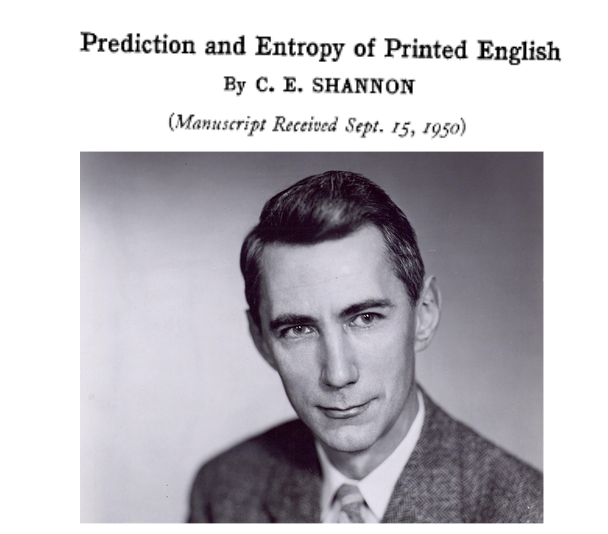
\includegraphics[scale = 0.4]{pics/shannon.png}
    \caption{Imagen de Shannon.}
    \label{fig:shannon}
\end{figure}

Por otro lado, en su libro \textit{Syntactic Structures} (1957), Noam Chomsky (en la Figura~\ref{fig:chomsky}), un lingüista y científico cognitivo, cuestionó la capacidad de los modelos de lenguaje probabilísticos para capturar y comprender la gramática del lenguaje humano \cite{chomsky2009syntactic}. Según Chomsky, la noción de ``gramaticalmente correcto'' no puede ser equiparada a ``significativo'' en un sentido probabilista. Para ilustrar esto, presentó dos oraciones ficticias, ambas carentes de sentido:

\begin{enumerate}
    \item Colorless green ideas sleep furiously.
    \item Furiously sleep ideas green colorless.
\end{enumerate}

Aunque ambas oraciones carecen de significado, Chomsky argumentó que solo la primera se considera gramaticalmente correcta por los hablantes de inglés. Además, enfatizó que la corecctitud gramatical en inglés no puede determinarse únicamente mediante aproximaciones estadísticas. Aunque es poco probable que ninguna de las dos oraciones (1) o (2) haya surgido en documentos escritos en inglés, un modelo estadístico como los modelos de lenguaje vistos en este capítulo las consideraría igualmente ``remotas'' en relación al inglés. Sin embargo, la oración (1) es gramaticalmente correcta, mientras que la oración (2) no lo es, lo que destaca las limitaciones de los enfoques estadísticos para capturar la gramática. Estos argumentos retrasaron el estudio de los modelos de lenguaje probabilísticos durante varios años \cite{JurafskyBook}.

\begin{figure}[h]
    \centering
    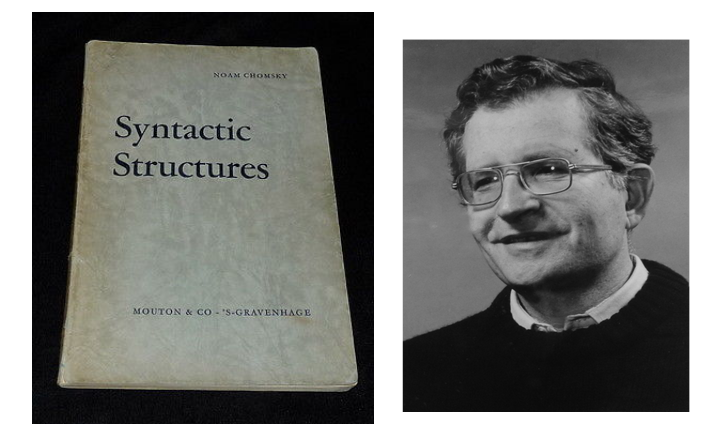
\includegraphics[scale = 0.4]{pics/chomsky.png}
    \caption{Imagen de Chomsky}
    \label{fig:chomsky}
\end{figure}


\section{Conclusiones}
El cálculo de probabilidades en modelos de lenguaje probabilísticos implica tres pasos:
    \begin{enumerate}
        \item Expandir $p(w_1, w_2, \ldots, w_n)$ usando la regla de la Cadena.
        \item Aplicar los supuestos Independencia de Markov \\
        $p(w_i | w_1, w_2, \ldots, w_{i-2}, w_{i-1}) = p(w_i | w_{i-2}, w_{i-1})$.
        \item Suavizar las estimaciones utilizando conteos de orden inferior.
    \end{enumerate}

No obstante, los modelos de lenguaje de bigramas o trigramas (que consideran dos palabras anteriores como contexto) tienen limitaciones en contextos largos y no pueden aprovechar contextos similares. Por ejemplo, consideremos los contextos:
\begin{itemize}
 \item $c_1$: Después de comer cereales
\item  $c_2$: Luego de desayunar avena
\end{itemize}

Aunque esperaríamos que las distribuciones de probabilidad $p(w|c_1)$ y $p(w|c_2)$ fueran similares, dado que $c_1$ y $c_2$ casi no comparten palabras, los modelos de n-gramas que se limitan a contar frecuencia de palabras no pueden capturar estas similitudes entre contextos.


Otros métodos para mejorar los modelos de lenguaje incluyen introducir variables latentes para representar tópicos, conocidos como modelos de tópicos \cite{blei2003latent} presentados en el Capítulo~\ref{cap_ir}. O alternativamente, reemplazar $p(w_i | w_1, w_2, \ldots, w_{i-2}, w_{i-1})$ con una red neuronal predictiva y una ``capa de embedding'' para representar mejor contextos más grandes y aprovechar similitudes entre palabras en el contexto. \cite{bengio2000neural}

Los modelos de lenguaje modernos utilizan redes neuronales profundas en su estructura principal y tienen un vasto espacio de parámetros como se verá en el Capítulo~\ref{cap_llm}.





\chapter{Text Classification and Naïve Bayes}
\label{cap_nb}
\begin{itemize}
    \item La clasificación es fundamental tanto para la inteligencia humana como para la artificial.
    \item Decidir qué letra, palabra o imagen se ha presentado a nuestros sentidos, reconocer caras o voces, clasificar el correo, asignar calificaciones a las tareas.
    \item Estos son ejemplos de asignar una categoría a una entrada.
    \item El objetivo de la clasificación es tomar una única observación, extraer algunas características útiles y así clasificar la observación en una de las clases discretas establecidas.
    \item La mayoría de los casos de clasificación en el procesamiento del lenguaje se realizan mediante aprendizaje automático supervisado.
    \item Estas diapositivas se basan en el material del curso de Daniel Jurafsky: \url{https://web.stanford.edu/~jurafsky/slp3/4.pdf}
\end{itemize}

Ejemplo 1: Clasificación de spam

\begin{figure}[h]
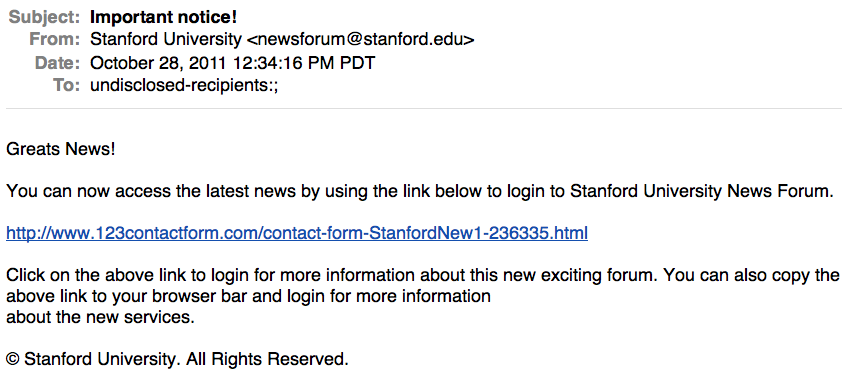
\includegraphics[scale = 0.35]{pics/spam.png}
\end{figure}


Ejemplo 2: ¿Quién escribió los documentos Federalist?

\begin{itemize}
    \item 1787-8: Ensayos anónimos intentaron convencer a Nueva York de ratificar la Constitución de EE. UU.: Jay, Madison, Hamilton.
    \item La autoría de 12 de las cartas está en disputa.
    \item 1963: Resuelto por Mosteller y Wallace mediante métodos bayesianos.
\end{itemize}

\begin{center}
    \begin{figure}[h]
        \begin{minipage}{0.3\textwidth}
            \centering
            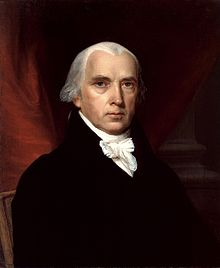
\includegraphics[width=\linewidth]{pics/madison.png}
            \caption{James Madison}
        \end{minipage}\hfill
        \begin{minipage}{0.3\textwidth}
            \centering
            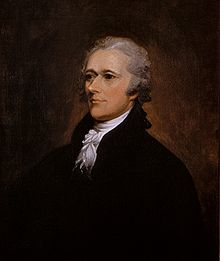
\includegraphics[width=\linewidth]{pics/hamilton.png}
            \caption{Alexander Hamilton}
        \end{minipage}
    \end{figure}
\end{center}


Ejemplo 3: ¿Cuál es el tema de este artículo médico?

\begin{figure}[h]
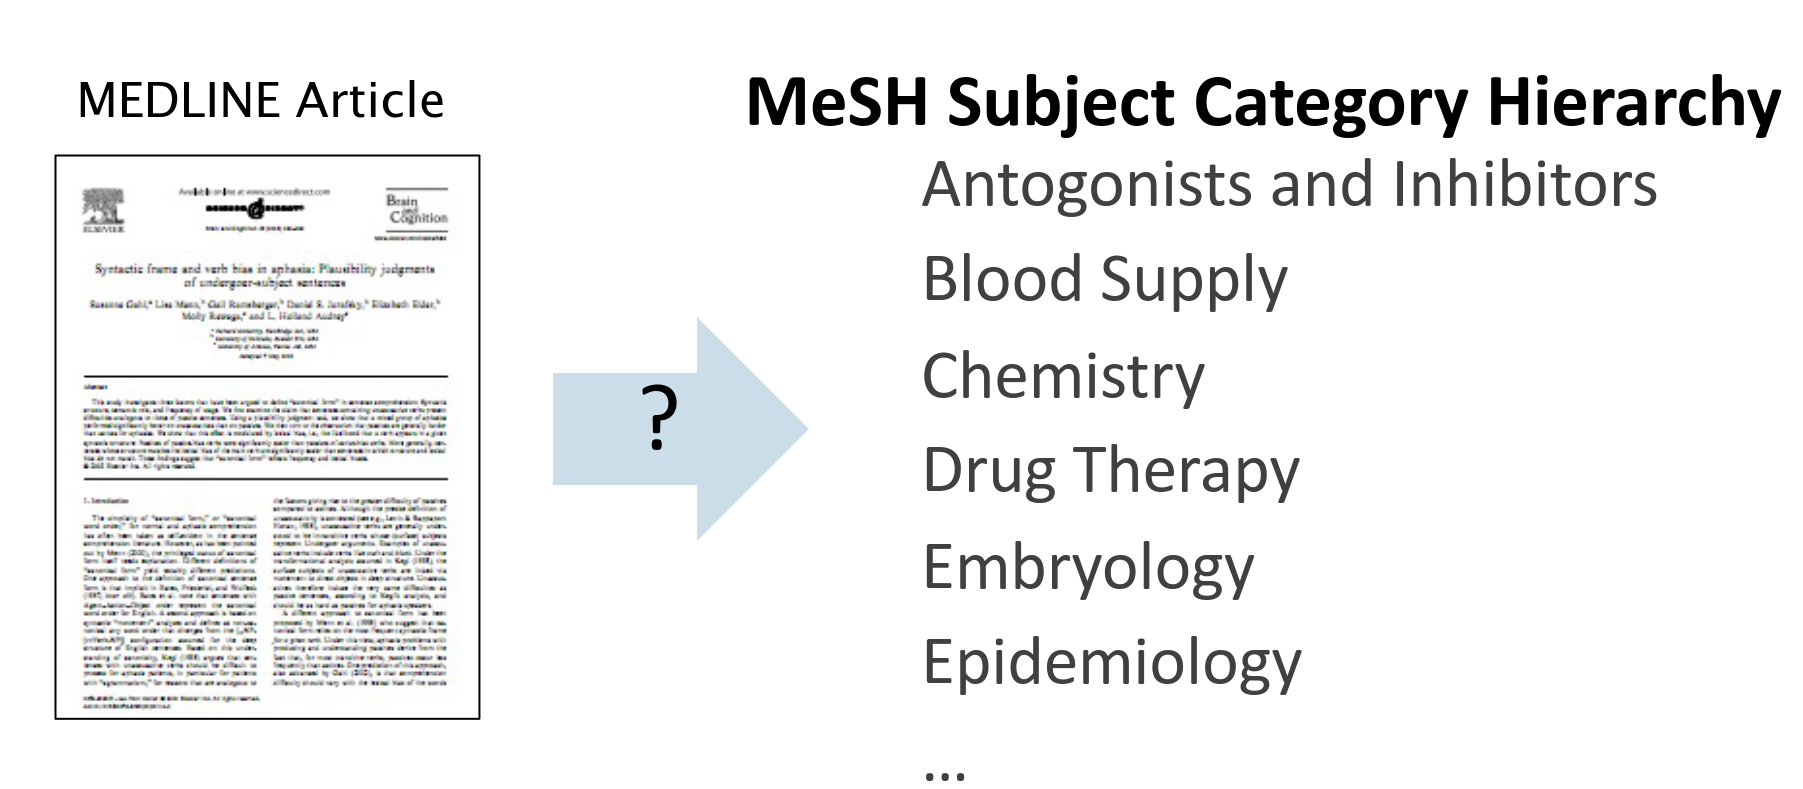
\includegraphics[scale = 0.2]{pics/medarticle.png}
\end{figure}



Ejemplo 4: ¿Reseña de película positiva o negativa?

\begin{itemize}
    \item \textcolor{blue}{\textbf{+}} ...personajes extravagantes y sátira \textcolor{blue}{rico} aplicada, y algunos \textcolor{blue}{grandes} giros de la trama.
    \item \textcolor{red}{\textbf{-}} Fue \textcolor{red}{patético}. La peor parte fue las escenas de boxeo...
    \item \textcolor{blue}{\textbf{+}} ...salsa de caramelo \textcolor{blue}{increíble} y almendras dulces y tostadas. ¡Me \textcolor{blue}{encanta} este lugar!
    \item \textcolor{red}{\textbf{-}} ...pizza \textcolor{red}{horrible} y \textcolor{red}{ridículamente} cara...
\end{itemize}



\paragraph{¿Por qué el análisis de sentimientos?}

\begin{itemize}
    \item Película: ¿Esta reseña es positiva o negativa?
    \item Productos: ¿Qué opinan las personas sobre el nuevo iPhone?
    \item Sentimiento público: ¿Cómo está la confianza del consumidor?
    \item Política: ¿Qué opinan las personas sobre este candidato o tema?
    \item Predicción: Predecir resultados electorales o tendencias del mercado a partir del sentimiento.
\end{itemize}


\paragraph{Clasificación básica de sentimientos}

El análisis de sentimientos es la detección de actitudes.

\begin{itemize}
    \item Tarea simple en la que nos enfocamos en esta clase.
    \begin{itemize}
        \item ¿Es la actitud de este texto positiva o negativa?
    \end{itemize}
\end{itemize}



\paragraph{Resumen: Clasificación de texto}

La clasificación de texto se puede aplicar a varias tareas, incluyendo:

\begin{itemize}
    \item Análisis de sentimientos
    \item Detección de spam
    \item Identificación de autoría
    \item Identificación de idioma
    \item Asignación de categorías, temas o géneros
    \item ...
\end{itemize}


\section{Clasificación de texto: Definición}

\textbf{Entrada}:
\begin{itemize}
    \item Un documento $d$
    \item Un conjunto fijo de clases $C = \{c_1, c_2, \ldots, c_J\}$
\end{itemize}

\textbf{Salida}: Una clase predicha $c \in C$


\subsection{Métodos de clasificación: Reglas codificadas a mano}

Reglas basadas en combinaciones de palabras u otras características.

\begin{itemize}
    \item Spam: \textit{dirección-en-lista-negra} O (\textit{“dólares” Y “has sido seleccionado”})
    \item La precisión puede ser alta si las reglas se refinan cuidadosamente por expertos
    \item Pero construir y mantener estas reglas es costoso
\end{itemize}

\subsection{Métodos de clasificación: Aprendizaje automático supervisado}

\textbf{Entrada}:
\begin{itemize}
    \item Un documento $d$
    \item Un conjunto fijo de clases $C = \{c_1, c_2, \ldots, c_J\}$
    \item Un conjunto de entrenamiento de $m$ documentos etiquetados manualmente: $(d_1, c_1), (d_2, c_2), \ldots, (d_m, c_m)$
\end{itemize}

\textbf{Salida}:
\begin{itemize}
    \item Un clasificador aprendido $\gamma: d \to c$
\end{itemize}

Cualquier tipo de clasificador se puede utilizar:
\begin{itemize}
    \item Naïve Bayes
    \item Regresión logística
    \item Redes neuronales
    \item k-vecinos más cercanos
    % Agrega más clasificadores según sea necesario
\end{itemize}

\subsection{Problemas de aprendizaje supervisado}
\begin{itemize}
    \item Tenemos ejemplos de entrenamiento $x^{(i)}$, $y^{(i)}$ para $i = 1, \ldots, m$. Cada $x^{(i)}$ es una entrada, cada $y^{(i)}$ es una etiqueta.
    \item La tarea es aprender una función $f$ que asigna las entradas $x$ a las etiquetas $f(x)$.
    \item Modelos condicionales:
    \begin{itemize}
        \item Aprender una distribución $p(y|x)$ a partir de ejemplos de entrenamiento.
        \item Para cualquier entrada de prueba $x$, definir $f(x) = \arg \max_y p(y|x)$.
    \end{itemize}
\end{itemize}

\subsection{Modelos generativos}
\begin{itemize}
    \item Dados ejemplos de entrenamiento $x^{(i)}$, $y^{(i)}$ para $i = 1, \ldots, m$, la tarea es aprender una función $f$ que asigna las entradas $x$ a las etiquetas $f(x)$.
    \item Modelos generativos:
    \begin{itemize}
        \item Aprender la distribución conjunta $p(x, y)$ a partir de los ejemplos de entrenamiento.
        \item A menudo, tenemos $p(x, y) = p(y)p(x|y)$.
        \item Nota: Luego tenemos
        \[
        p(y|x) = \frac{p(y)p(x|y)}{p(x)} \quad \text{donde} \quad p(x) = \sum_y p(y)p(x|y).
        \]
    \end{itemize}
\end{itemize}

\subsection{Clasificación con Modelos Generativos}
\begin{itemize}
    \item Dados ejemplos de entrenamiento $x^{(i)}$, $y^{(i)}$ para $i = 1, \ldots, m$. La tarea consiste en aprender una función $f$ que mapee las entradas $x$ a las etiquetas $f(x)$.
    \item Modelos generativos:
    \begin{itemize}
        \item Aprenden la distribución conjunta $p(x, y)$ a partir de los ejemplos de entrenamiento.
        \item A menudo, tenemos $p(x, y) = p(y)p(x|y)$.
    \end{itemize}
    \item La salida del modelo es:
    \[
    \begin{aligned}
    f(x) = \arg\max_y p(y|x) &= \arg\max_y \frac{p(y)p(x|y)}{p(x)} \\
    &= \arg\max_y p(y)p(x|y)
    \end{aligned}
    \]
\end{itemize}


\section{Intuición del Bayes Ingenuo}
El Bayes Ingenuo es un método de clasificación simple ("ingenuo") basado en la regla de Bayes.
\begin{itemize}
    \item Se basa en una representación muy simple de un documento: \textit{Bolsa de palabras}.
\end{itemize}

\paragraph{La Representación de Bolsa de Palabras}

\begin{figure}[h]
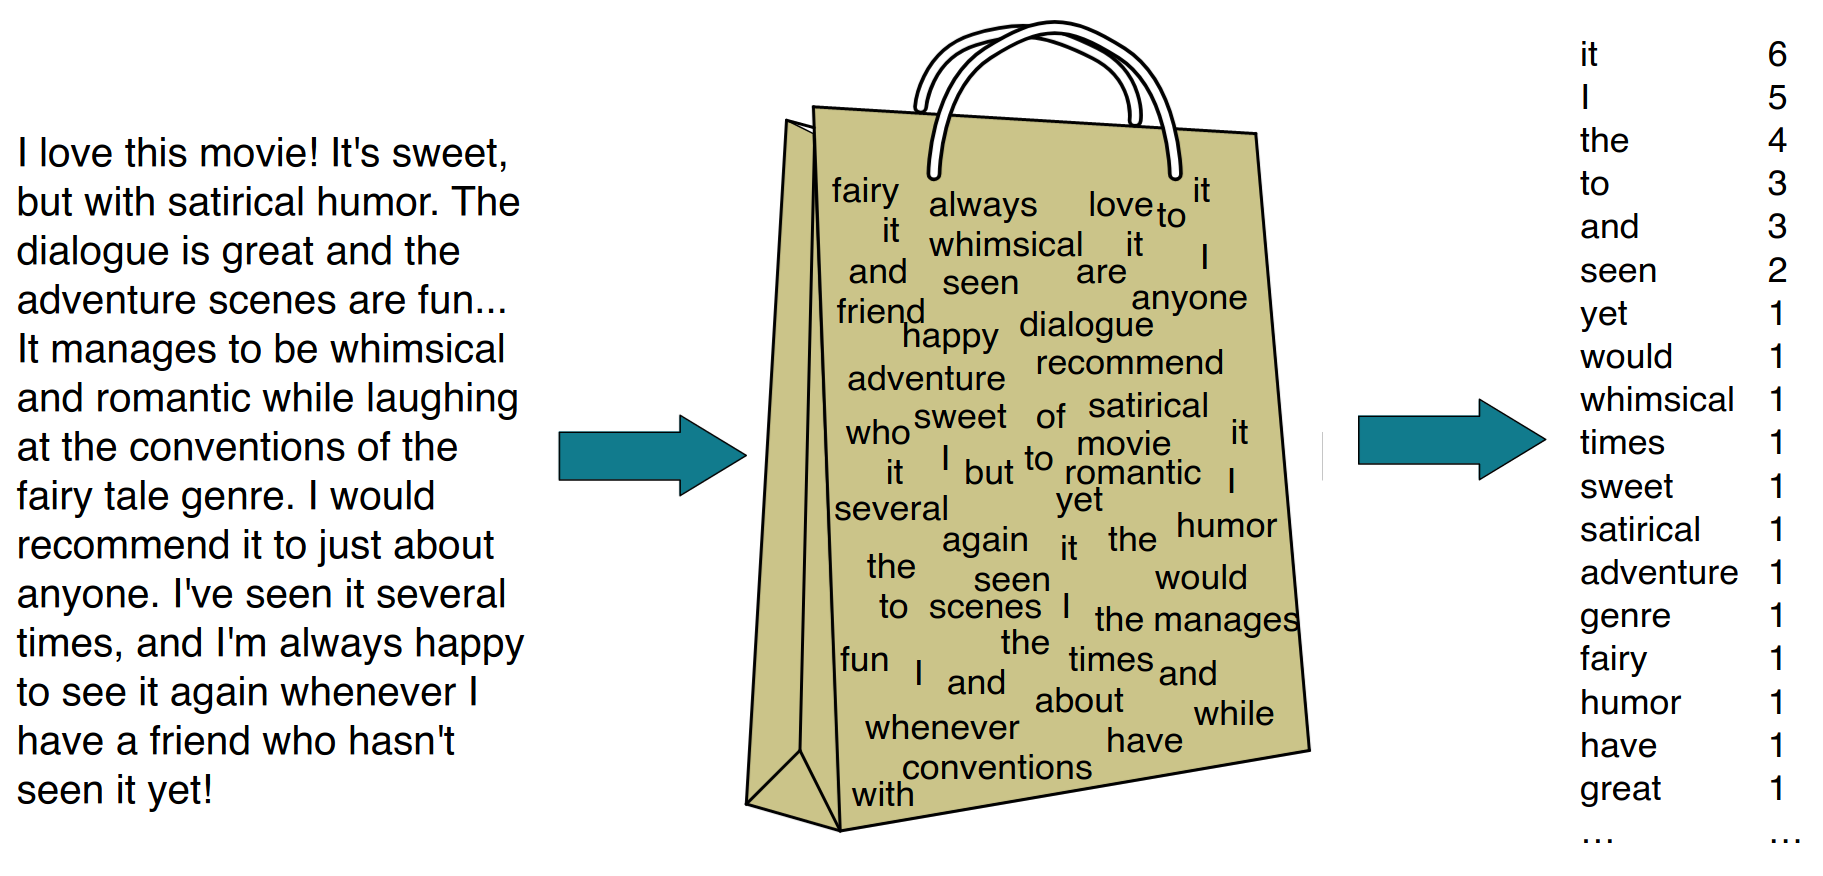
\includegraphics[scale = 0.22]{pics/bow.png}
\end{figure}


\subsection{Aplicación de la Regla de Bayes a Documentos y Clases}
Para un documento $d$ y una clase $c$:
\[
P(c | d) = \frac{P(d | c)P(c)}{P(d)}
\]


\section{Clasificador Bayes Ingenuo}
\begin{itemize}
    \item MAP significa ``máximo a posteriori'', que representa la clase más probable:
    \[
    c_{\text{MAP}} = \arg\max_{c \in C} P(c | d)
    \]
    \item Para calcular la clase más probable, aplicamos la regla de Bayes:
    \[
    = \arg\max_{c \in C} \frac{P(d | c)P(c)}{P(d)}
    \]
    \item Finalmente, podemos eliminar el denominador ya que permanece constante para todas las clases:
    \[
    = \arg\max_{c \in C} P(d | c)P(c)
    \]
    \item Para clasificar el documento $d$, usamos la estimación MAP:
    \[
    c_{\text{MAP}} = \arg\max_{c \in C} P(d | c)P(c)
    \]
    \item El documento $d$ se representa como un conjunto de características $x_1, x_2, \ldots, x_n$.
    \item El clasificador calcula la probabilidad condicional de las características dada una clase y la probabilidad a priori de la clase:
    \[
    = \arg\max_{c \in C} P(x_1, x_2, \ldots, x_n | c)P(c)
    \]
    \item El término $P(x_1, x_2, \ldots, x_n | c)$ representa la

 "verosimilitud" de las características dada la clase.
    \item El término $P(c)$ representa la probabilidad "a priori" de la clase.
    \item El clasificador Bayes Ingenuo \cite{mccallum1998comparison} calcula la estimación MAP considerando las probabilidades de verosimilitud y a priori:
    \[
    c_{\text{MAP}} = \arg\max_{c \in C} P(x_1, x_2, \ldots, x_n | c)P(c)
    \]
    \item La probabilidad de las características dada la clase, $P(x_1, x_2, \ldots, x_n | c)$, puede estimarse contando las frecuencias relativas en un corpus.
    \item La probabilidad a priori de la clase, $P(c)$, representa con qué frecuencia ocurre esta clase.
    \item Sin algunas suposiciones simplificadoras, estimar la probabilidad de cada posible combinación de características en $P(x_1, x_2, \ldots, x_n | c)$ requeriría un gran número de parámetros y conjuntos de entrenamiento imposiblemente grandes.
    \item Por lo tanto, los clasificadores Bayes Ingenuo realizan dos suposiciones simplificadoras.
\end{itemize}


\subsection{Suposiciones de Independencia del Bayes Ingenuo Multinomial}
\begin{itemize}
    \item Suposición de Bolsa de Palabras: asumimos que la posición de las palabras en el documento no importa.
    \item Suposición de Independencia Condicional: asumimos que las probabilidades de las características $P(x_i | c_j)$ son independientes dada la clase $c_j$.
    \item En el clasificador Bayes Ingenuo Multinomial, la probabilidad de un documento con características $x_1, x_2, \ldots, x_n$ dada la clase $c$ se puede calcular como:
    \[
    P(x_1, x_2, \ldots, x_n | c) = P(x_1 | c) \cdot P(x_2 | c) \cdot P(x_3 | c) \cdot \ldots \cdot P(x_n | c)
    \]
\end{itemize}

\subsection{Clasificador Bayes Ingenuo Multinomial}
\begin{itemize}
    \item La estimación del Máximo A Posteriori (MAP) para la clase $c$ en el clasificador Bayes Ingenuo Multinomial se calcula como:
    \[
    c_{\text{MAP}} = \arg\max_{c \in C} P(x_1, x_2, \ldots, x_n | c)P(c)
    \]
    \item Alternativamente, podemos escribirlo como:
    \[
    c_{\text{NB}} = \arg\max_{c \in C} P(c_j) \prod_{x \in X} P(x | c)
    \]
    \item $P(c_j)$ representa la probabilidad a priori de la clase $c_j$.
    \item $\prod_{x \in X} P(x | c)$ representa la verosimilitud de las características $x_1, x_2, \ldots, x_n$ dadas la clase $c$.
\end{itemize}


\subsection{Aplicación de los clasificadores Naive Bayes multinomiales a la clasificación de texto}

El clasificador Naive Bayes multinomial para la clasificación de texto se puede aplicar de la siguiente manera:
\[
c_{\text{NB}} = \arg\max_{c_j \in C} P(c_j) \prod_{i \in \text{positions}} P(x_i | c_j)
\]
Donde:
\begin{itemize}
    \item $c_{\text{NB}}$ representa la clase predicha para el documento de prueba.
    \item $C$ es el conjunto de todas las clases posibles.
    \item $P(c_j)$ es la probabilidad previa de la clase $c_j$.
    \item $\prod_{i \in \text{positions}} P(x_i | c_j)$ calcula la probabilidad de cada característica $x_i$ en la posición $i$ dada la clase $c_j$.
    \item El producto se toma sobre todas las posiciones de palabras en el documento de prueba.
\end{itemize}

\subsection{Problemas al multiplicar muchas probabilidades}

Multiplicar muchas probabilidades puede resultar en un desbordamiento de punto flotante, especialmente cuando se manejan probabilidades pequeñas. Por ejemplo, $0.0006 \times 0.0007 \times 0.0009 \times 0.01 \times 0.5 \times 0.000008 \ldots$.

Para solucionar este problema, podemos utilizar logaritmos, ya que $\log(ab) = \log(a) + \log(b)$. En lugar de multiplicar las probabilidades, podemos sumar los logaritmos de las probabilidades. Así, el clasificador Naive Bayes multinomial se puede expresar utilizando logaritmos de la siguiente manera:
\[
c_{\text{NB}} = \arg\max_{c_j \in C} \left(\log(P(c_j)) + \sum_{i \in \text{position}} \log(P(x_i | c_j))\right)
\]

Al tomar logaritmos, evitamos el problema del desbordamiento de punto flotante y realizamos cálculos en el espacio logarítmico. El clasificador se convierte en un modelo lineal, donde la predicción es el argmax de la suma de pesos (logaritmos de probabilidades) y las entradas (logaritmos de probabilidades condicionales). Por lo tanto, Naive Bayes es un clasificador lineal que opera en el espacio logarítmico.

\subsection{Aprendizaje del modelo Naive Bayes multinomial}

El primer intento: Estimaciones de máxima verosimilitud
\begin{itemize}
    \item Las probabilidades se estiman utilizando las frecuencias observadas en los datos de entrenamiento.
    \item La probabilidad previa de una clase $c_j$ se estima como:
    \[
    \hat{P}(c_j) = \frac{N_{c_j}}{N_{\text{total}}}
    \]
    donde $N_{c_j}$ es el número de documentos en la clase $c_j$ y $N_{\text{total}}$ es el número total de documentos.
    \item La estimación de la probabilidad de la palabra $w_i$ dada la clase $c_j$ se calcula como:
    \[
    \hat{P}(w_i | c_j) = \frac{{\text{count}(w_i, c_j)}}{\sum_{w\in V}{\text{count}(w, c_j)}}
    \]
    donde $w \in V$ representa una palabra en el vocabulario $V$.
    \item El denominador es la suma de las frecuencias de todas las palabras en el vocabulario dentro de la clase $c_j$.
\end{itemize}

\subsection{Estimación de parámetros}

Para estimar los parámetros del modelo Naive Bayes multinomial, seguimos estos pasos:

\begin{itemize}
  \item Creamos un mega-documento para cada tema $c_j$ concatenando todos los documentos de ese tema.
  \item Calculamos la frecuencia de la palabra $w_i$ en el mega-documento, que representa la fracción de veces que la palabra $w_i$ aparece entre todas las palabras en los documentos del tema $c_j$.
  \item La probabilidad estimada $\hat{P}(w_i | c_j)$ de la palabra $w_i$ dada la clase $c_j$ se obtiene dividiendo el recuento de ocurrencias de $w_i$ en el mega-documento del tema $c_j$ por el recuento total de palabras en el mega-documento:
  \[
  \hat{P}(w_i | c_j) = \frac{{\text{count}(w_i, c_j)}}{\sum_{w\in V}{\text{count}(w, c_j)}}
  \]
  Aquí, $\text{count}(w_i, c_j)$ representa el número de veces que la palabra $w_i$ aparece en el mega-documento del tema $c_j$, y $\text{count}(w, c_j)$ es el recuento total de palabras en el mega-documento.
\end{itemize}

\subsection{Probabilidades cero y el problema de las palabras no vistas}

Consideremos el escenario en el que no hemos encontrado la palabra "fantástico" en ningún documento de entrenamiento clasificado como positivo (pulgar hacia arriba). Utilizando la estimación de máxima verosimilitud, la probabilidad $\hat{P}(\text{``fantástico''} \mid \text{positivo})$ se calcularía como:
\[
\hat{P}(\text{``fantástico''} \mid \text{positivo}) = \frac{\text{count}(\text{``fantástico''}, \text{positivo})}{\sum_{w \in V} \text{count}(w, \text{positivo})}
\]

En este caso, el recuento de la palabra ``fantástico'' en los documentos positivos es cero, lo que conduce a una probabilidad cero:
\[
\hat{P}(\text{``fantástico''} \mid \text{positivo}) = \frac{0}{\sum_{w \in V} \text{count}(w, \text{positivo})} = 0
\]

Sin embargo, las probabilidades cero no pueden eliminarse, independientemente de la evidencia adicional presente. Esto plantea un problema al calcular la estimación del máximo a posteriori (MAP), que se utiliza para la clasificación:
\[
c_{\text{MAP}} = \arg\max_c \left(\hat{P}(c) \prod_{i} \hat{P}(x_i \mid c)\right)
\]

Con una probabilidad cero para una palabra, toda la expresión se vuelve cero, independientemente de la otra evidencia.

\subsection{Suavizado Laplaciano (Add-1) para Naïve Bayes}

Manejo de probabilidades cero con el suavizado Laplaciano (Add-1):
\begin{itemize}
    \item Para abordar el problema de las probabilidades cero, podemos utilizar la técnica de suavizado Laplaciano (Add-1).
    \item La estimación suavizada $\hat{P}(w_i \mid c)$ se calcula como:
    \[
    \hat{P}(w_i \mid c) = \frac{\text{count}(w_i, c) + 1}{\sum_{w \in V} (\text{count}(w, c) + 1)}
    \]
    \item Aquí, se agrega un recuento adicional de 1 tanto al numerador como al denominador.
    \item El denominador se ajusta agregando el tamaño del vocabulario $V$ para garantizar una normalización adecuada.
    \item Al hacerlo, evitamos las probabilidades cero y permitimos que cierta masa de probabilidad se distribuya a palabras no vistas.
    \item Esta técnica de suavizado ayuda a mitigar el problema de las palabras no vistas y evita la eliminación completa de ciertas clases durante la clasificación.
\end{itemize}

\subsection{Naïve Bayes multinomial: aprendizaje}

Aprendiendo el modelo Naïve Bayes multinomial:
\begin{itemize}
    \item Para aprender los parámetros del modelo, necesitamos calcular los términos $P(c_j)$ y $P(w_k \mid c_j)$.
    \item Para cada clase $c_j$ en el conjunto de clases $C$, realizamos los siguientes pasos:
    \begin{itemize}
        \item Recuperamos todos los documentos $docs_j$ que pertenecen a la clase $c_j$.
        \item Calculamos el término $P(w_k \mid c_j)$ para cada palabra $w_k$ en el vocabulario $V$:
        \[
        P(w_k \mid c_j) = \frac{{n_k + \alpha}}{{n + \alpha \cdot \lvert \text{Vocabulary} \rvert}}
        \]
        donde $n_k$ representa el número de ocurrencias de la palabra $w_k$ en el documento concatenado $Text_j$.
        \item Calculamos la probabilidad a priori $P(c_j)$:
        \[
        P(c_j) = \frac{{\lvert docs_j \rvert}}{{\lvert \text{total number of documents} \rvert}}
        \]
    \end{itemize}
    \item Para calcular $P(w_k \mid c_j)$, necesitamos extraer el vocabulario $V$ del corpus de entrenamiento.
\end{itemize}

\subsection{Palabras desconocidas}

Tratamiento de palabras desconocidas en los datos de prueba:
\begin{itemize}
    \item Cuando encontramos palabras desconocidas en los datos de prueba que no aparecen en los datos de entrenamiento o en el vocabulario, las ignoramos.
    \item Eliminamos estas palabras desconocidas del documento de prueba como si no estuvieran presentes en absoluto.
    \item No asignamos ninguna probabilidad a estas palabras desconocidas en el proceso de clasificación.
\end{itemize}

Esto es una visión general del modelo Naive Bayes multinomial y su aplicación a la clasificación de texto. Cabe destacar que existen variantes y extensiones más sofisticadas de Naive Bayes que se adaptan a diferentes requisitos y características de los datos.


\section{Ejemplo}

\textbf{Datos de Entrenamiento:} 

\begin{table}[h]
\centering
\begin{tabular}{|c|p{0.7\textwidth}|}
\hline
\textbf{Categoría} & \textbf{Texto} \\
\hline
Negative & Just plain boring, entirely predictable and lacks energy. \\
\hline
Negative & No surprises and very few laughs. \\
\hline
Positive & Very powerful. \\
\hline
Positive & The most fun film of the summer. \\
\hline
\end{tabular}
\end{table}


\textbf{Test:} 
\begin{table}[h]
\centering
\begin{tabular}{|c|p{0.7\textwidth}|}
\hline
\textbf{Categoría} & \textbf{Texto} \\
\hline
? & Predictable with no fun. \\
\hline
\end{tabular}
\end{table}

\begin{figure}[h]
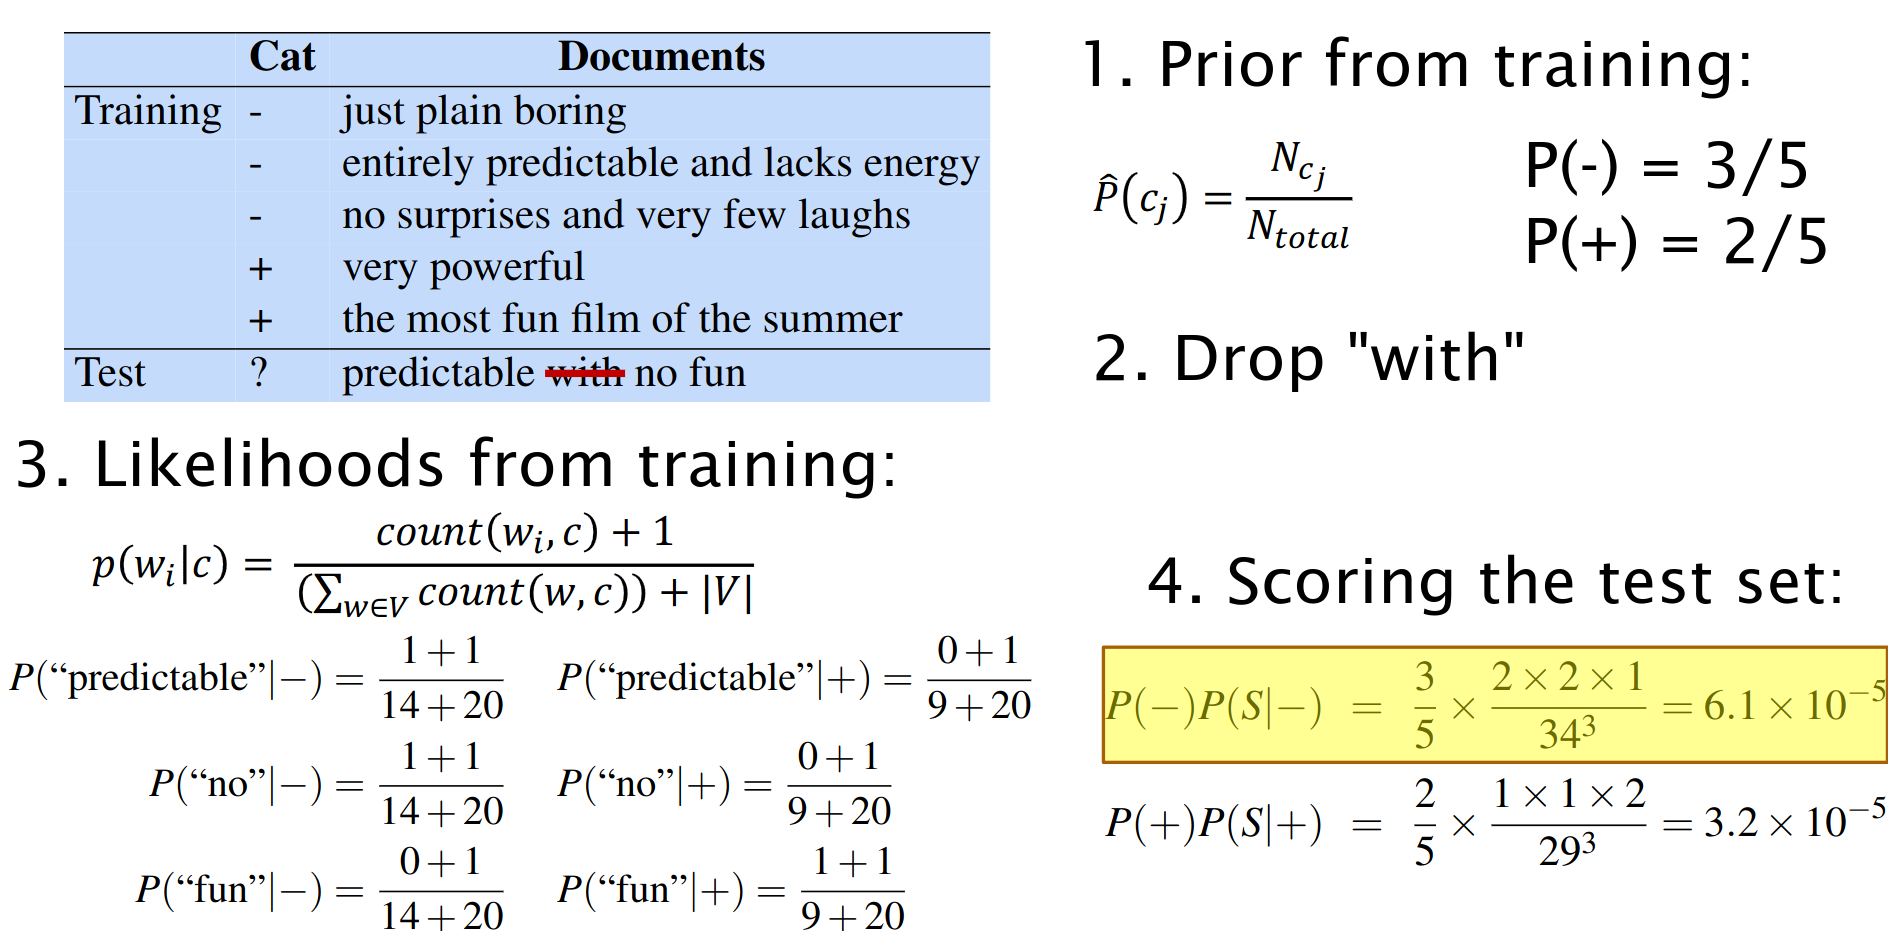
\includegraphics[scale = 0.23]{pics/naive_example.png}
\end{figure}

\section{Naive Bayes como modelo de lenguaje}

Cuando utilizamos características de palabras individuales y consideramos todas las palabras en el texto, el naive Bayes tiene una similitud importante con la modelización del lenguaje.

Específicamente, un modelo naive Bayes se puede ver como un conjunto de modelos de lenguaje de unigramas específicos de cada clase, en el que el modelo para cada clase instancia un modelo de lenguaje de unigrama.

Las características de verosimilitud del modelo naive Bayes asignan una probabilidad a cada palabra $P(\text{word}|c)$, y el modelo también asigna una probabilidad a cada oración:

\[P(s|c) = \prod_{i\in \text{positions}} P(w_i|c)\]

Consideremos un modelo naive Bayes con las clases positiva (+) y negativa (-) y los siguientes parámetros del modelo:

\begin{center}
\begin{tabular}{ccc}
\textbf{w} & $P(w|+)$ & $P(w|-)$ \\
I & 0.1 & 0.2 \\
love & 0.1 & 0.001 \\
this & 0.01 & 0.01 \\
fun & 0.05 & 0.005 \\
film & 0.1 & 0.1 \\
... & ... & ...
\end{tabular}
\end{center}

Cada una de las dos columnas anteriores instancian un modelo de lenguaje que puede asignar una probabilidad a la oración "I love this fun film":

\[P("\text{I love this fun film}"|+) = 0.1 \times 0.1 \times 0.01 \times 0.05 \times 0.1 = 0.0000005\]
\[P("\text{I love this fun film}"|-) = 0.2 \times 0.001 \times 0.01 \times 0.005 \times 0.1 = 0.0000000010\]

Como sucede, el modelo positivo asigna una probabilidad más alta a la oración:
\[P(s|\text{pos}) > P(s|\text{neg})\]

Cabe destacar que esto es solo la parte de verosimilitud del modelo naive Bayes; una vez que multiplicamos por la probabilidad a priori, un modelo naive Bayes completo podría tomar una decisión de clasificación diferente.



\section{Evaluación}

\begin{itemize}
 \item Consideremos solo tareas de clasificación de texto binario.
 \item Imagina que eres el CEO de Delicious Pie Company.
 \item Quieres saber lo que la gente está diciendo sobre tus pasteles.
 \item Por lo tanto, construyes un detector de tweets de "Delicious Pie" con las siguientes clases:
\begin{itemize}
\item Clase positiva: tweets sobre Delicious Pie Co.
\item Clase negativa: todos los demás tweets.
\end{itemize}
\end{itemize}



\subsection{La Matriz de Confusión 2x2}
\begin{table}[h]
\centering
\begin{tabular}{|c|c|c|}
\hline
\textbf{} & \textbf{Sistema Positivo} & \textbf{Sistema Negativo} \\
\hline
\textbf{Oro Positivo} & Verdadero Positivo (VP) & Falso Negativo (FN) \\
\hline
\textbf{Oro Negativo} & Falso Positivo (FP) & Verdadero Negativo (VN) \\
\hline
\end{tabular}
\end{table}

\textbf{Recall} (también conocido como \textbf{Sensibilidad} o \textbf{Tasa de Verdaderos Positivos}):
\[ \text{Recall} = \frac{VP}{VP + FN} \]

\textbf{Precisión}:
\[ \text{Precisión} = \frac{VP}{VP + FP} \]

\textbf{Exactitud}:
\[ \text{Exactitud} = \frac{VP + VN}{VP + FP + VN + FN} \]


\subsection{Evaluación: Exactitud}
¿Por qué no usamos la exactitud como nuestra métrica?

Imagina que vimos 1 millón de tweets:
\begin{itemize}
\item 100 de ellos hablaban sobre Delicious Pie Co.
\item 999,900 hablaban de otra cosa.
\end{itemize}

Podríamos construir un clasificador tonto que simplemente etiquete todos los tweets como "no sobre pasteles":
\begin{itemize}
\item ¡¡¡Obtendría una exactitud del 99.99\%!!! ¡¡¡Wow!!!
\item ¡Pero sería inútil! ¡No devuelve los comentarios que estamos buscando!
\end{itemize}

Por eso usamos precisión y recall en su lugar.

\subsection{Evaluación: Precisión y Recall}
\textbf{Precisión} mide el porcentaje de elementos que el sistema detectó (es decir, los elementos que el sistema etiquetó como positivos) que son realmente positivos (según las etiquetas de oro humanas).

\[
\text{Precisión} = \frac{\text{Verdaderos Positivos}}{\text{Verdaderos Positivos + Falsos Positivos}}
\]

\textbf{Recall} mide el porcentaje de elementos que el sistema identificó correctamente de todos los elementos que deberían haber sido identificados.

\[
\text{Recall} = \frac{\text{Verdaderos Positivos}}{\text{Verdaderos Positivos + Falsos Negativos}}
\]

\subsection{¿Por qué Precisión y Recall?}
Considera nuestro clasificador tonto de pasteles que simplemente etiqu

eta nada como "sobre pasteles".

\begin{itemize}
  \item Exactitud = 99.99\% (etiqueta correctamente la mayoría de los tweets como no relacionados con pasteles)
  \item Recall = 0 (no detecta ninguno de los 100 tweets relacionados con pasteles)
\end{itemize}

La precisión y el recall, a diferencia de la exactitud, enfatizan los verdaderos positivos:
\begin{itemize}
  \item Se centran en encontrar las cosas que se supone que debemos buscar.
\end{itemize}

\subsection{Una Medida Combinada: Medida F}
La medida F es un número único que combina la precisión (P) y el recall (R), definida como:
\[
F_\beta = \frac{(\beta^2+1)PR}{\beta^2P + R}
\]

La medida F, definida con el parámetro $\beta$, pondera diferencialmente la importancia del recall y la precisión.
\begin{itemize}
  \item $\beta > 1$ favorece al recall
  \item $\beta < 1$ favorece a la precisión
\end{itemize}

Cuando $\beta = 1$, la precisión y el recall son iguales, y tenemos la medida $F_1$ equilibrada:
\[
F_1 = \frac{2PR}{P + R}
\]

\subsection{Conjuntos de Prueba de Desarrollo ("Devsets")}

\begin{itemize}
 \item Para evitar el sobreajuste y proporcionar una estimación más conservadora del rendimiento, comúnmente utilizamos un enfoque de tres conjuntos: conjunto de entrenamiento, conjunto de desarrollo y conjunto de prueba.
\begin{figure}[h]
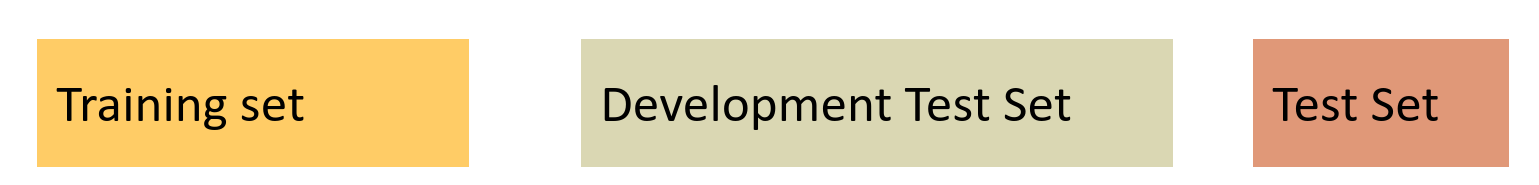
\includegraphics[scale = 0.23]{pics/devsets.png}
\end{figure}

\begin{itemize}
\item \textbf{Conjunto de entrenamiento}: Se utiliza para entrenar el modelo.
\item \textbf{Conjunto de desarrollo}: Se utiliza para ajustar el modelo y seleccionar los mejores hiperparámetros.
\item \textbf{Conjunto de prueba}: Se utiliza para informar el rendimiento final del modelo.
\end{itemize}

\item Este enfoque garantiza que el modelo no esté ajustado específicamente al conjunto de prueba, evitando el sobreajuste.
\item Sin embargo, crea una paradoja: queremos la mayor cantidad de datos posible para el entrenamiento, pero también para el conjunto de desarrollo.
\item ¿Cómo dividimos los datos?

\end{itemize}





\subsection{Validación Cruzada: Múltiples Divisiones}

\begin{itemize}
\item La validación cruzada nos permite utilizar todos nuestros datos para el entrenamiento y la prueba sin tener un conjunto de entrenamiento, conjunto de desarrollo y conjunto de prueba fijos.
\item Elegimos un número $k$ y dividimos nuestros datos en $k$ subconjuntos disjuntos llamados pliegues.
\item En cada iteración, uno de los pliegues se selecciona como conjunto de prueba mientras que los $k-1$ pliegues restantes se utilizan para entrenar el clasificador.
\item Calculamos la tasa de error en el conjunto de prueba y repetimos este proceso $k$ veces.
\item Finalmente, promediamos las tasas de error de estas $k$ ejecuciones para obtener una tasa de error promedio.
\item Por ejemplo, la validación cruzada de 10 pliegues implica entrenar 10 modelos con el 90\% de los datos y probar cada modelo por separado.
\item Las tasas de error resultantes se promedian para obtener la estimación final del rendimiento.
\item Sin embargo, la validación cruzada requiere que todo el corpus sea ciego, lo que impide examinar los datos para sugerir características o comprender el comportamiento del sistema.
\item Para abordar esto, se crea un conjunto de entrenamiento y un conjunto de prueba fijos, y se realiza la validación cruzada de 10 pliegues dentro del conjunto de entrenamiento.
\item La tasa de error se calcula convencionalmente en el conjunto de prueba.
\end{itemize}


\begin{center}
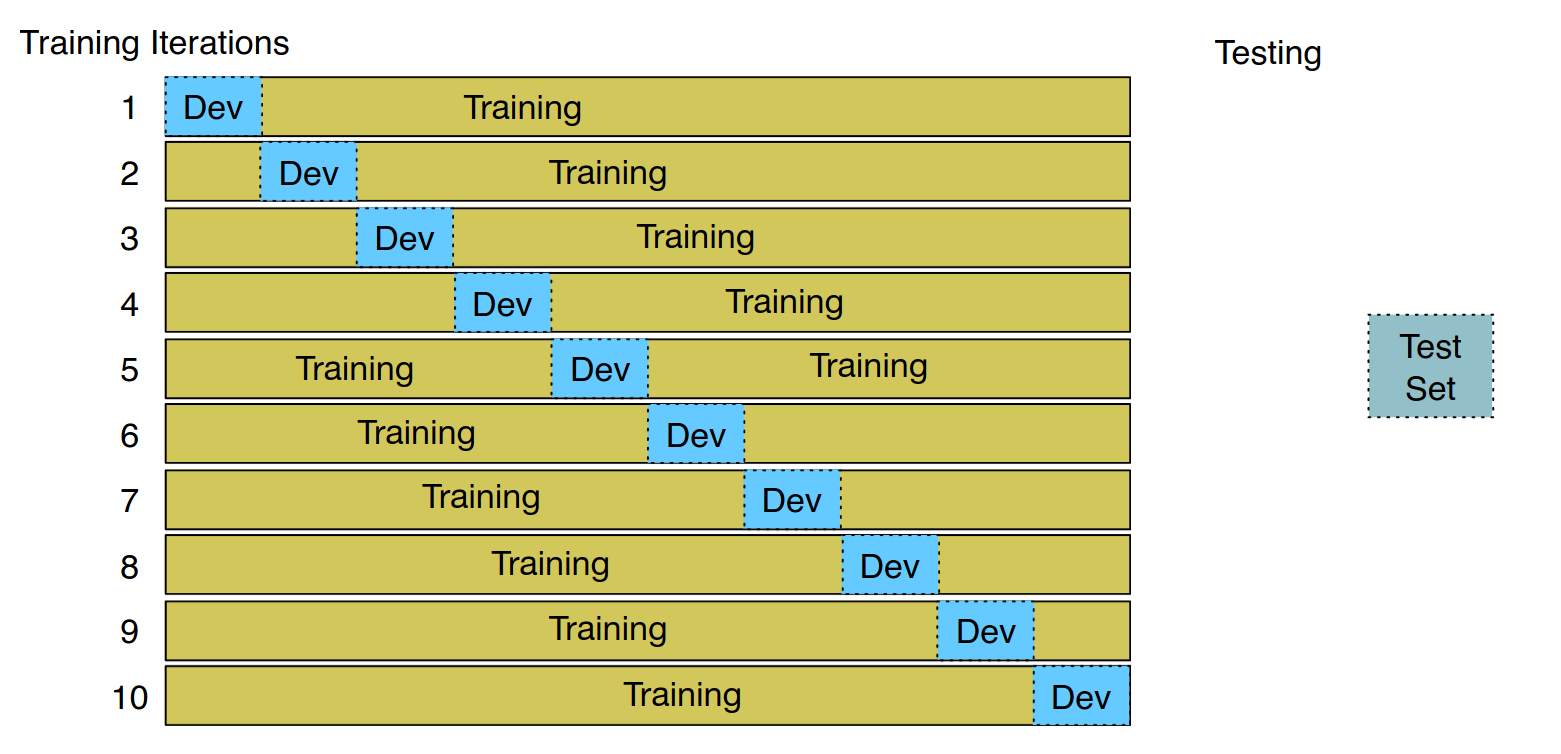
\includegraphics[scale=0.28]{pics/cv.png}
\end{center}


\subsection{Matriz de Confusión para clasificación de 3 clases}


\begin{center}
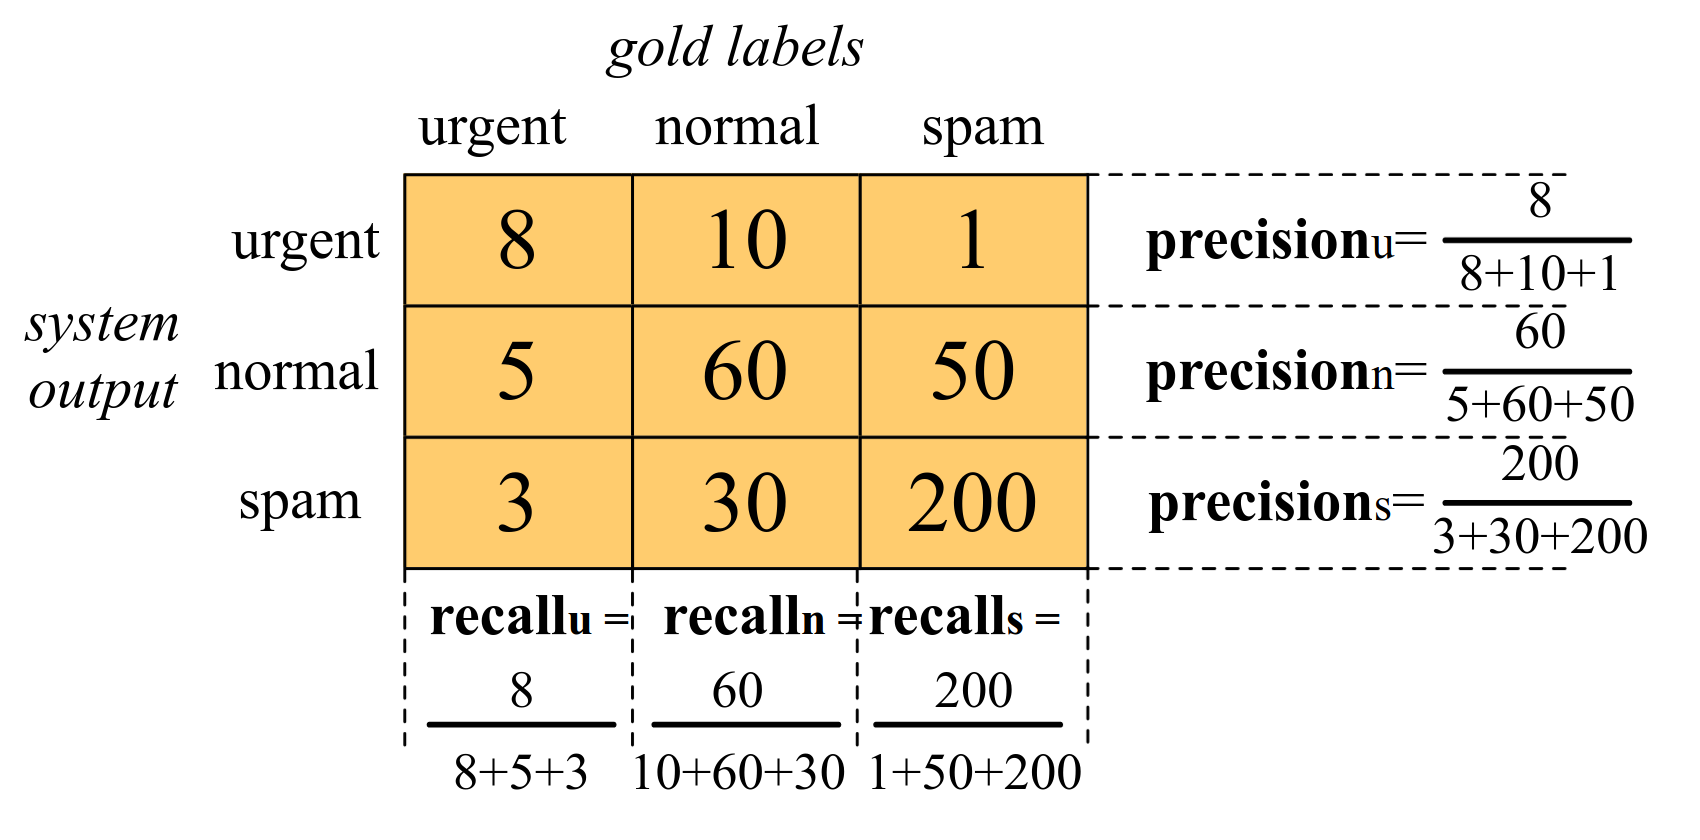
\includegraphics[scale=0.23]{pics/confmatrix.png}
\end{center}

Cómo combinar métricas binarias (Precisión, Recall, $F_1$) de más de 2 clases para obtener una métrica única:
\begin{itemize}
 \item Macro-promedio:
 \begin{itemize}
    \item Calcular las métricas de rendimiento (Precisión, Recall, $F_1$) para cada clase individualmente.
    \item Promediar las métricas en todas las clases.
 \end{itemize}
 \item Micro-promedio:
 \begin{itemize}
    \item Recopilar las decisiones para todas las clases en una matriz de confusión.
    \item Calcular la Precisión y el Recall a partir de la matriz de confusión.
 \end{itemize}
\end{itemize}

\begin{center}
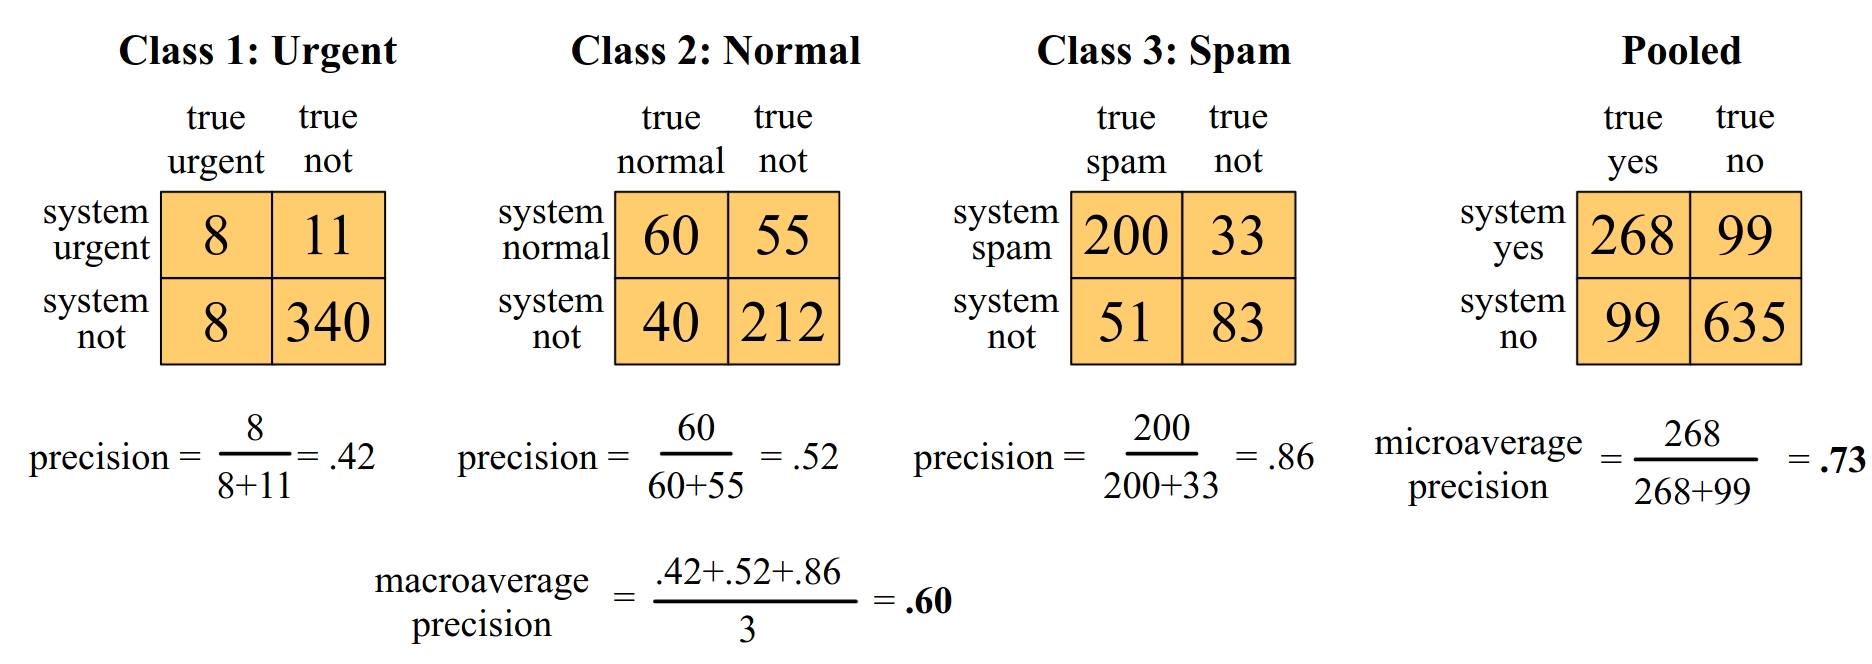
\includegraphics[scale=0.23]{pics/confmatrixmulti.png}
\end{center}



\chapter{Modelos Lineales}
\label{cap_lineales}

 Cuando hacemos aprendizaje supervisado, en escencia tenemos que buscar sobre el conjunto de todas las posibles funciones que pueden mapear desde las entradas hacia las salidas. Si no acotamos el espacio de busqueda de alguna forma nos encontramos con  un problema muy difícil (y bastante mal definido) \cite{goldberg2017neural}. A menudo nos limitamos a buscar dentro de familias específicas de funciones. Por ejemplo, el espacio de todas las funciones lineales con $d_{in}$ entradas y $d_{out}$ salidas. Estas familias de funciones se llaman clases de hipótesis. Al restringirnos a una clase de hipótesis específica, estamos inyectando al aprendiz con sesgo inductivo, es decir, un conjunto de suposiciones sobre la forma de la solución deseada. Algunas clases de hipótesis facilitan procedimientos eficientes para buscar la solución.

Una clase de hipótesis común es la de una función lineal de alta dimensión:

\begin{equation}
\begin{split}
f(\vec{x}) = \vec{x} \cdot W + \vec{b}\\
\vec{x} \in  \mathcal{R}^{d_{in}} & \quad W \in  \mathcal{R}^{d_{in}\times d_{out}} \quad \vec{b} \in  \mathcal{R}^{d_{out}}
\end{split}
\end{equation}

El vector $\vec{x}$ es la entrada de la función. La matriz $W$ y el vector $\vec{b}$ son los parámetros. El objetivo del aprendiz es establecer los valores de los parámetros $W$ y $\vec{b}$ de manera que la función se comporte como se pretende en una colección de valores de entrada $\vec{x}_{1:k} = \vec{x}_1,\dots,\vec{x}_k$ y las correspondientes salidas deseadas $\vec{y}_{1:k} = \vec{y}_1,\dots,\vec{y}_k$. La tarea de buscar en el espacio de funciones se reduce así a buscar en el espacio de parámetros.

\section{Ejemplo: Detección de Idiomas}

Consideremos la tarea de distinguir entre documentos escritos en inglés y documentos escritos en alemán. Este es un problema de clasificación binaria:

\begin{equation}
\begin{split}
f(\vec{x}) = \vec{x} \cdot \vec{w} + b
\end{split}
\end{equation}

donde $d_{out} = 1$, donde $\vec{w}$ es un vector y $b$ es un escalar. El rango de la función lineal es $[-\infty, \infty]$. Para usarla en la clasificación binaria, es común pasar la salida de $f(x)$ a través de la función $signo$, mapeando los valores negativos a -1 (clase negativa) y los valores no negativos a +1 (clase positiva).

Las frecuencias de letras son buenos predictores (características) para esta tarea, pero aún más informativos son los recuentos de bigramas de letras, es decir, pares de letras consecutivas. Es probable que nos encontremos con un documento nuevo sin ninguna de las palabras que observamos en el conjunto de entrenamiento, mientras que un documento sin ninguno de los distintivos bigramas de letras es significativamente menos probable \cite{goldberg2017neural}. Supongamos que tenemos un alfabeto de 28 letras (a-z, espacio y un símbolo especial para todos los demás caracteres, incluidos dígitos, puntuación, etc.). Los documentos se representan como vectores de dimensión $28 \times 28$, es decir, $\vec{x} \in \mathcal{R}^{784}$. Cada entrada $\vec{x}_{[i]}$ representa un recuento de una combinación particular de letras en el documento, normalizado por la longitud del documento. Por ejemplo, si denotamos por $\vec{x}_{ab}$ la entrada de $\vec{x}$ correspondiente al bigrama de letras $ab$:

\begin{equation}
\vec{x}_{ab} = \frac{\#ab}{|D|}
\end{equation}

donde $\#ab$ es el número de veces que aparece el bigrama $ab$ en el documento y $|D|$ es el número total de bigramas en el documento (la longitud del documento).

La figura muestra histogramas de bigramas de caracteres para documentos en inglés y alemán. Los guiones bajos representan espacios. Solo se muestran los bigramas de caracteres más frecuentes.

\begin{figure}[htb]
	\centering
	 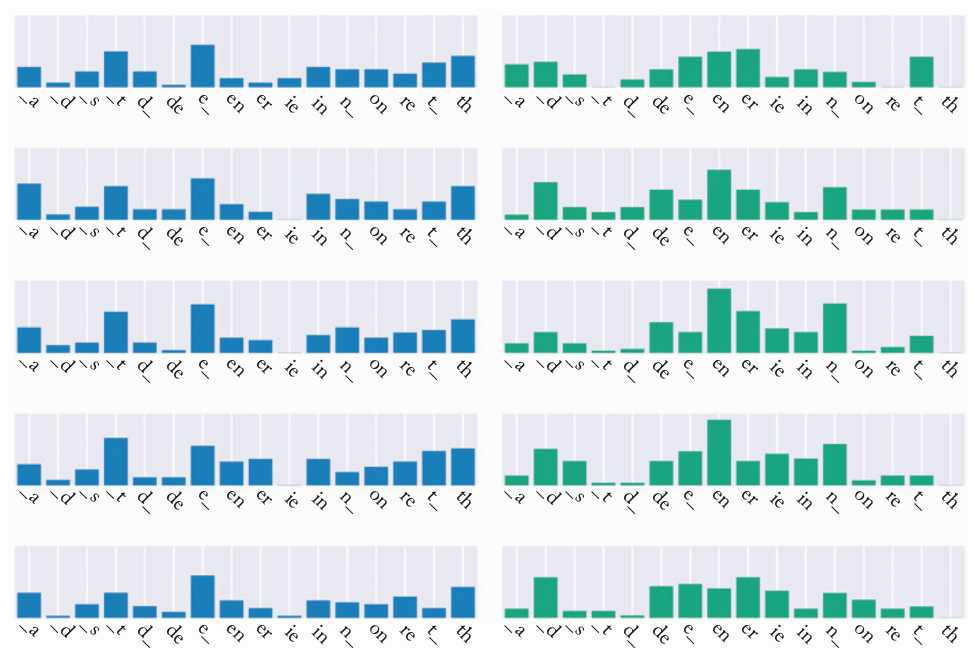
\includegraphics[scale=0.26]{pics/langbigrams.png}
\end{figure}

Fuente: \cite{goldberg2017neural}

La figura anterior muestra patrones claros en los datos. Dado un nuevo elemento, por ejemplo:

\begin{figure}[htb]
	\centering
	 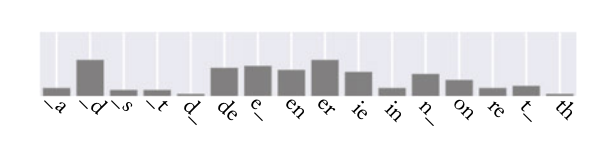
\includegraphics[scale=0.4]{pics/langbigramstest.png}
\end{figure}

Probablemente podríamos decir que es más similar al grupo alemán que al grupo inglés (observar la frecuencia de "th" y "ie"). No podemos usar una regla única definitiva como "si tiene th es inglés" o "si tiene ie es alemán". Aunque los textos en alemán tienen considerablemente menos "th" que el inglés, la combinación "th" puede ocurrir en textos en alemán, al igual que la combinación "ie" puede ocurrir en inglés. La decisión requiere ponderar diferentes factores relativos entre sí.

Podemos formalizar el problema en un entorno de aprendizaje automático utilizando un modelo lineal:

\begin{equation}
\begin{split}
\hat{y} = \text{sign}(\vec{x}\cdot \vec{w} + b) = \text{sign}(\vec{x}_{aa}\times \vec{w}_{aa}+ \vec{x}_{ab}\times \vec{w}_{ab}+ \vec{x}_{ac}\times \vec{w}_{ac} \dots +b)
\end{split}
\end{equation}

Un documento se considerará inglés si $f(\vec{x}) \geq 0$ y alemán en caso contrario. La intuición detrás del aprendizaje es la siguiente:

\begin{enumerate}
\item El aprendizaje debe asignar valores positivos grandes a las entradas de $\vec{w}$ asociadas con pares de letras que son mucho más comunes en inglés que en alemán (por ejemplo, "th").
\item También debe asignar valores negativos a los pares de letras que son mucho más comunes en alemán que en inglés (por ejemplo, "ie", "en").
\item Finalmente, debe asignar valores alrededor de cero a los pares de letras que son comunes o raros en ambos idiomas.
\end{enumerate}


%Translate this Latex book chapter to Spanish. Output in Latex format. Rearrange bullet points (\items) into full paragraphs. Make sure that sentences are connected in a more fluid way as they come.
\section{Clasificación binaria log-lineal}
La salida $f(\vec{x})$ se encuentra en el rango $[-\infty,\infty]$, y la mapeamos a una de las dos clases $\{-1,+1\}$ utilizando la función $signo$. Esto es adecuado si lo único que nos importa es la clase asignada. Sin embargo, puede que también estemos interesados en la confianza de la decisión o en la probabilidad que el clasificador asigna a la clase.

Una alternativa que facilita esto es mapear la salida al rango $[0,1]$ mediante una función de compresión como la función sigmoide $\sigma(x)$:

\begin{equation}
\sigma(x) = \frac{1}{1+e^{-x}}
\end{equation}

lo que resulta en:

\begin{equation}
\hat{y}=\sigma(f(\vec{x})) = \frac{1}{1+e^{-\vec{x}\cdot \vec{w}+b}}
\end{equation}

La función sigmoide es monótona creciente y mapea los valores al rango $[0, 1]$, con $0$ mapeado a $\frac{1}{2}$. Cuando se utiliza con una función de pérdida adecuada (que se discutirá más adelante), las predicciones binarias realizadas mediante el modelo log-lineal se pueden interpretar como estimaciones de la probabilidad de pertenencia a la clase:

\begin{equation}
 \sigma(f(\vec{x})) = P(\hat{y} = 1| \vec{x}) \quad \text{de que $\vec{x}$ pertenezca a la clase positiva.}
\end{equation}

También obtenemos $P(\hat{y} = 0| \vec{x}) = 1 - P(\hat{y} = 1| \vec{x}) = 1-\sigma(f(\vec{x}))$. Cuanto más cercano sea el valor a $0$ o $1$, más seguro está el modelo en su predicción de pertenencia a la clase, y el valor $0.5$ indica incertidumbre del modelo.

\section{Clasificación multiclase}
La mayoría de los problemas de clasificación son de naturaleza multiclase: se asignan ejemplos a una de las $k$ clases diferentes. Por ejemplo, se nos puede dar un documento y se nos pide clasificarlo en uno de los seis posibles idiomas: inglés, francés, alemán, italiano, español y otros.

Una solución posible es considerar seis vectores de pesos $\vec{w}_{EN}$, $\vec{w}_{FR}$, $\dots$ y sesgos (uno para cada idioma). Predecimos el idioma que resulta en el puntaje más alto:

\begin{equation}
 \hat{y} = f(\vec{x}) = \operatorname{argmax}_{L \in \{ EN,FR,GR,IT,SP,O \}} \quad \vec{x}\cdot \vec{w}_L+ b_{L}
\end{equation}

Los seis conjuntos de parámetros $\vec{w}_L \in  \mathcal{R}^{784}$ y $b_L$ se pueden organizar en una matriz $W \in \mathcal{R}^{784\times6}$ y un vector $\vec{b} \in \mathcal R^6$, y la ecuación se puede reescribir como:

\begin{equation}
 \begin{split}
  \vec{\hat{y}} = f(\vec{x}) = \quad & \vec{x} \cdot W + \vec{b}\\
   \text{predicción} = \hat{y} = \quad  & \operatorname{argmax}_i \vec{\hat{y}}_{[i]}
 \end{split}
\end{equation}

Aquí, $\vec{\hat{y}} \in \mathcal{R}^6$ es un vector de los puntajes asignados por el modelo a cada idioma, y determinamos el idioma predicho tomando el argmax sobre las entradas de $\vec{\hat{y}}$ (las columnas con el valor más alto).

\section{Representaciones}
Consideremos el vector $\vec{\hat{y}}$ resultante de aplicar un modelo entrenado a un documento. Podemos considerar que este vector es una representación del documento, ya que captura las propiedades del documento que son importantes para nosotros, es decir, los puntajes de los diferentes idiomas. La representación $\vec{\hat{y}}$ contiene estrictamente más información que la predicción $\operatorname{argmax}_i \vec{\hat{y}}_{[i]}$.

Por ejemplo, $\vec{\hat{y}}$ se puede utilizar para distinguir documentos en los que el idioma principal es el alemán, pero que también contienen una cantidad considerable de palabras en francés. El agrupamiento de documentos basado en $\vec{\hat{y}}$ podría ayudar a descubrir documentos escritos en dialectos regionales o por autores multilingües.

Los vectores $\vec{x}$ que contienen los recuentos normalizados de los bigramas de letras para los documentos también son representaciones de los documentos. Se podría argumentar que contienen un tipo de información similar a los vectores $\vec{\hat{y}}$. Sin embargo, las representaciones en $\vec{\hat{y}}$ son más compactas (6 entradas en lugar de 784) y más especializadas para el objetivo de predicción de idioma. El agrupamiento por los vectores $\vec{x}$ probablemente revelaría similitudes en los documentos que no se deben a una mezcla particular de idiomas, sino tal vez al tema o estilo de escritura del documento.

La matriz entrenada $W \in \mathcal{R}^{784 \times 6}$ también se puede considerar como una representación aprendida. Podemos considerar dos vistas de $W$, como filas o como columnas.

\begin{figure}[htb]
	\centering
	 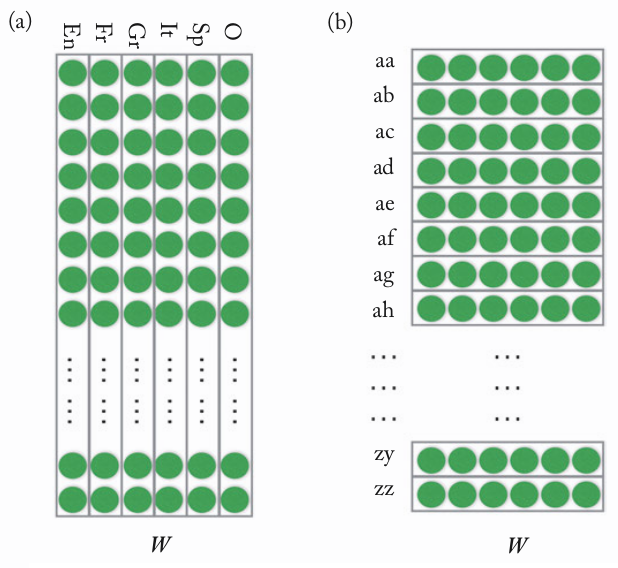
\includegraphics[scale=0.35]{pics/2rep.png}
\end{figure}

Dos vistas de la matriz $W$. (a) Cada columna corresponde a un idioma. (b) Cada fila corresponde a un bigrama de letras. Fuente: \cite{goldberg2017neural}.

Una columna de $W$ puede tomarse como una representación vectorial de $784$ dimensiones de un idioma en términos de sus patrones característicos de bigramas de letras. Luego, podemos agrupar los 6 vectores de idioma según su similitud. Cada una de las 784 filas de $W$ proporciona una representación vectorial de 6 dimensiones de ese bigrama en términos de los idiomas que promueve. Las representaciones son fundamentales para el aprendizaje profundo. Se podría argumentar que el principal poder del aprendizaje profundo es la capacidad de aprender buenas representaciones.

En el caso lineal, las representaciones son interpretables, ya que podemos asignar una interpretación significativa a cada dimensión en el vector de representación. Por ejemplo, cada dimensión puede corresponder a un idioma o a un determinado bigrama de letras.

Por otro lado, los modelos de aprendizaje profundo a menudo aprenden una cascada de representaciones de la entrada que se construyen una encima de la otra. Estas representaciones a menudo no son interpretables, es decir, no sabemos qué propiedades de la entrada capturan. Sin embargo, siguen siendo muy útiles para hacer predicciones.

\section{Representación de Vectores One-Hot}
El vector de entrada $\vec{x}$ en nuestro ejemplo de clasificación de idioma contiene los recuentos normalizados de los bigramas en el documento $D$. Este vector se puede descomponer en un promedio de $|D|$ vectores, cada uno correspondiente a una posición particular del documento $i$:

\begin{equation}
 \vec{x} = \frac{1}{|D|} \sum_{i=1}^{|D|} \vec{x}^{D_{[i]}}
\end{equation}

Aquí, $D_{[i]}$ es el bigrama en la posición $i$ del documento. Cada vector $\vec{x}^{D_{[i]}} \in \mathcal{R}^{784}$ es un vector one-hot, lo que significa que todos los elementos son cero excepto la única entrada que corresponde al bigrama de letras $D_{[i]}$, que es 1. El vector resultante $\vec{x}$ se conoce comúnmente como un promedio de bolsa de bigramas (más generalmente, una bolsa de palabras promediada, o simplemente una bolsa de palabras).

Las representaciones de bolsa de palabras contienen información sobre las identidades de todas las "palabras" (en este caso, bigramas) del documento, sin considerar su orden. Una representación one-hot se puede considerar como una bolsa de una sola "palabra".

\begin{figure}[htb]
	\centering
	 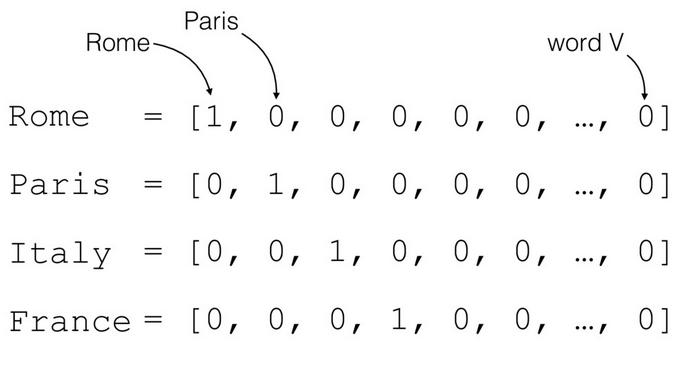
\includegraphics[scale=0.3]{pics/onehot.png}
\end{figure}

Vectores one-hot de palabras.

Fuente: \url{https://medium.com/@athif.shaffy/one-hot-encoding-of-text-b69124bef0a7}.

%Translate this Latex book chapter to Spanish. Output in Latex format. Rearrange bullet points (\items) into full paragraphs. Make sure that sentences are connected in a more fluid way as they come.\section{Clasificación Log-lineal de Múltiples Clases}
En el caso binario, transformamos la predicción lineal en una estimación de probabilidad al pasarla por la función sigmoide, lo que resulta en un modelo log-lineal. En el caso de múltiples clases, el análogo es pasar el vector de puntajes a través de la función \textbf{softmax}:

\begin{equation}
 \operatorname{softmax}(\vec{x})_{[i]} = \frac{e^{\vec{x}_{[i]}}}{\sum_j e^{\vec{x}_{[j]}}}
\end{equation}

Lo que resulta en:

\begin{equation}
\begin{split}
\vec{\hat{y}} \quad & =  \operatorname{softmax}(\vec{x} \cdot W + \vec{b})  \\
\vec{\hat{y}}_{[i]} \quad & = \frac{e^{(\vec{x} \cdot W + \vec{b})_{[i]}}}{\sum_j e^{(\vec{x} \cdot W + \vec{b})_{[j]}}}
\end{split}
\end{equation}

La transformación softmax fuerza a los valores en $\hat{\vec{y}}$ a ser positivos y sumar 1, lo que los hace interpretables como una distribución de probabilidad.

\section{Entrenamiento}
Cuando se entrena una función parametrizada (por ejemplo, un modelo lineal, una red neuronal), se define una función de pérdida $L(\hat{y}, y)$, que establece la pérdida al predecir $\hat{y}$ cuando la salida verdadera es $y$.

\begin{displaymath}
L(f(\vec{x};\Theta), y)
\end{displaymath}

Utilizamos el símbolo $\Theta$ para denotar todos los parámetros del modelo (por ejemplo, $W, \vec{b}$).

El objetivo del entrenamiento es minimizar la pérdida en los diferentes ejemplos de entrenamiento. Formalmente, una función de pérdida $L(\hat{y},y)$ asigna una puntuación numérica (un escalar) a una salida predicha $\hat{y}$ dada la salida esperada verdadera $y$. La función de pérdida debería alcanzar su valor mínimo para los casos en los que la predicción sea correcta.

También podemos definir una pérdida en todo el corpus con respecto a los parámetros $\Theta$ como la pérdida promedio en todos los ejemplos de entrenamiento:

\begin{displaymath}
 \mathcal{L}(\Theta) = \frac{1}{n} \sum_{i=1}^n L(f(\vec{x}_i;\Theta), y_i)
\end{displaymath}

El objetivo del algoritmo de entrenamiento es establecer los valores de los parámetros $\Theta$ de manera que el valor de $\mathcal{L}$ se minimice.

\begin{displaymath}
 \hat{\Theta} = \operatorname{argmin}_{\Theta} \mathcal{L}(\Theta) =  \operatorname{argmin}_{\Theta} \frac{1}{n} \sum_{i=1}^n L(f(\vec{x}_i;\Theta), y_i)
\end{displaymath}

\subsection{Optimización basada en Gradiente}
Las funciones se

entrenan utilizando métodos basados en gradientes. Estos métodos funcionan mediante el cálculo repetido de una estimación de la pérdida $L$ sobre el conjunto de entrenamiento. El método de entrenamiento calcula los gradientes de los parámetros ($\Theta$) con respecto a la estimación de pérdida y mueve los parámetros en la dirección opuesta al gradiente. Los diferentes métodos de optimización difieren en cómo se calcula la estimación de error y cómo se define el movimiento en la dirección opuesta al gradiente.

Si la función es convexa, el óptimo será global. De lo contrario, el proceso solo garantiza encontrar un óptimo local.

\begin{figure}[htb]
	\centering
	 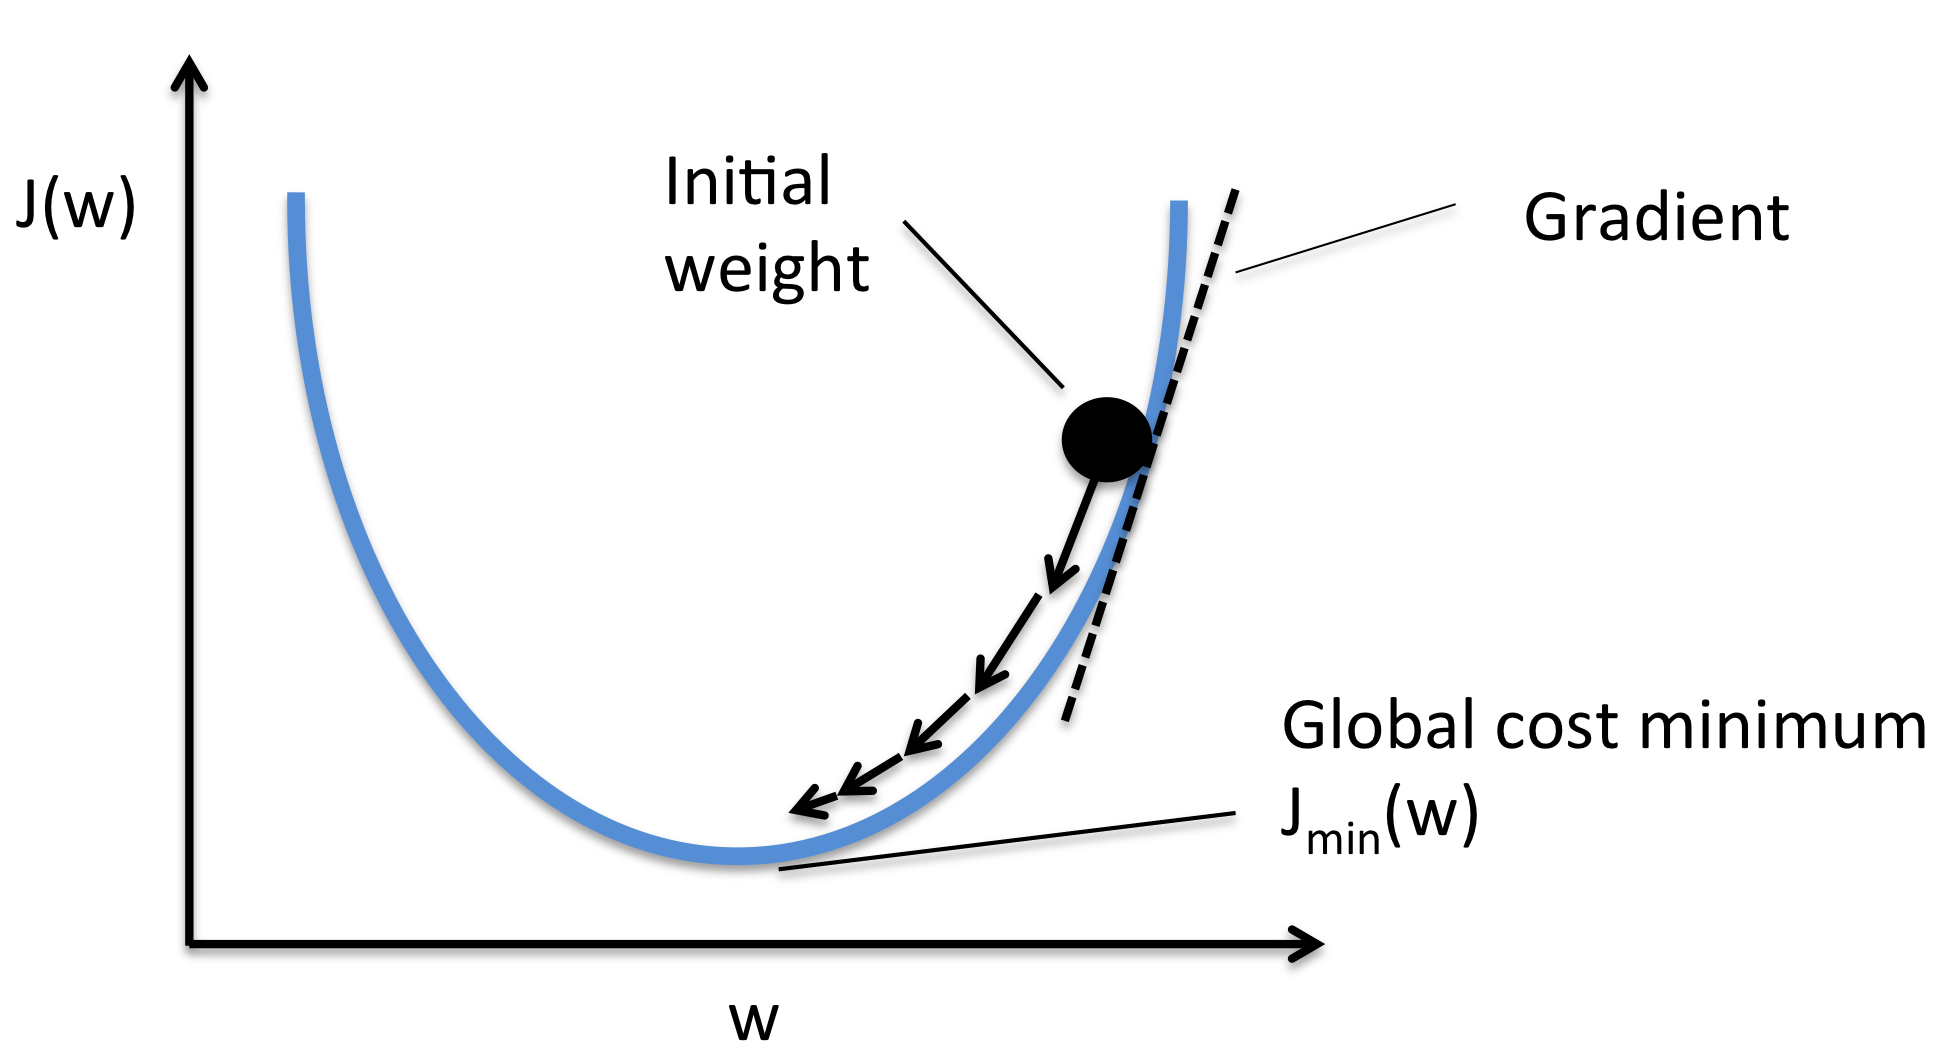
\includegraphics[scale=0.15]{pics/sgd.png}
\end{figure}
\footnotetext{Fuente: \url{https://sebastianraschka.com/images/faq/closed-form-vs-gd/ball.png}}

\begin{figure}[htb]
	\centering
	 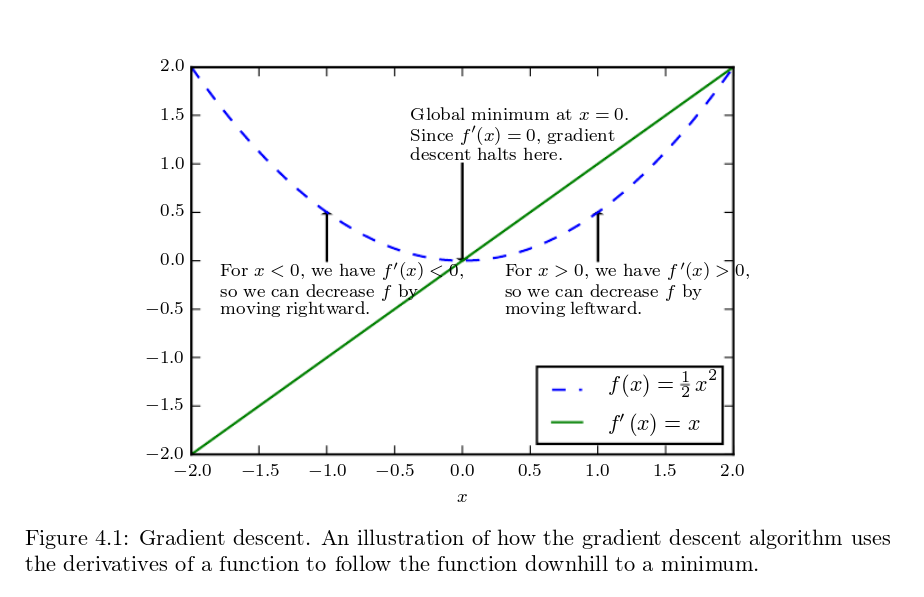
\includegraphics[scale=0.45]{pics/gradientdescent.png}
\end{figure}
\footnotetext{\cite{goodfellow2016deep}}

\subsection{Descenso de Gradiente Estocástico en Línea}
\begin{itemize}
\item Todos los parámetros se inicializan con valores aleatorios ($\Theta$).
\item Para cada ejemplo de entrenamiento $(x,y)$, calculamos la pérdida $L$ con los valores actuales de $\Theta$.
\item Luego actualizamos los parámetros con la siguiente regla hasta que se alcance la convergencia:
\item $\Theta_i \leftarrow \Theta_i - \eta \frac{\partial L}{\Theta_i}(\hat{y},y)$ (para todos los parámetros $\Theta_i$)
\end{itemize}

\begin{figure}[htb]
	\centering
	 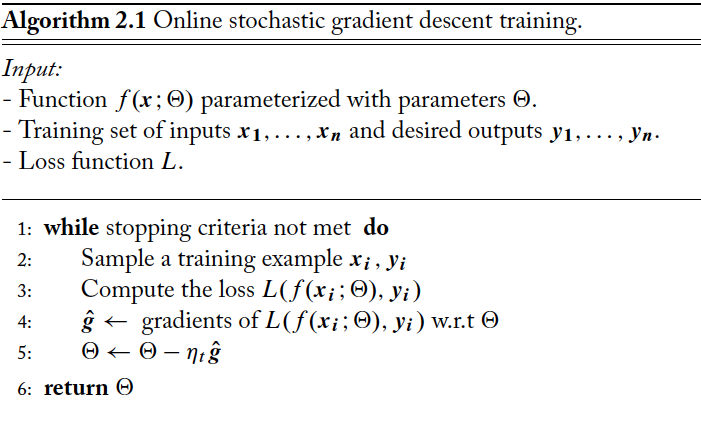
\includegraphics[scale=0.3]{pics/Online-SGD.png}
\end{figure}
\footnotetext{Fuente:\cite{goldberg2017neural}}

La tasa de aprendizaje puede ser fija durante todo el proceso de entrenamiento o puede decrecer como función del paso de tiempo $t$. El error calculado en la línea 3 se basa en un solo ejemplo de entrenamiento y, por lo tanto, es solo una estimación aproximada de la pérdida en todo el corpus $L$ que queremos minimizar. El ruido en el cálculo de la pérdida puede resultar en gradientes inexactos (los ejemplos individuales pueden proporcionar información ruidosa).

\subsection{Descenso de Gradiente Estocástico en Mini-batch}
\begin{itemize}
\item Una forma común de reducir este ruido es estimar el error y los gradientes en función de una muestra de $m$ ejemplos.
\item Esto da lugar al algoritmo de SGD en mini-batch.
\end{itemize}

\begin{figure}[htb]
	\centering
	 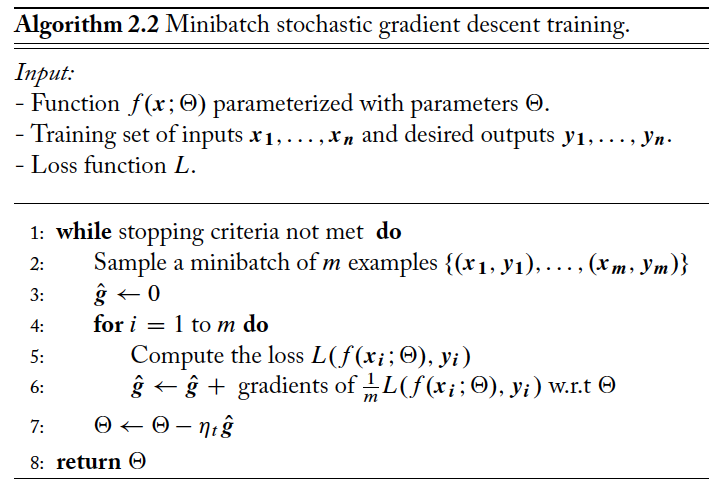
\includegraphics[scale=0.25]{pics/minibatch-SGD.png}
\end{figure}

Valores más altos de $m$ proporcionan mejores estimaciones de los gradientes en todo el corpus, mientras que valores más pequeños permiten más actualizaciones y, a su vez, una convergencia más rápida.

Para tamaños moderados de

$m$, algunas arquitecturas de cómputo (por ejemplo, GPUs) permiten una implementación paralela eficiente del cálculo en las líneas 3-6.

\footnotetext{Fuente:\cite{goldberg2017neural}}


%Translate this Latex book chapter to Spanish. Output in Latex format. Rearrange bullet points (\items) into full paragraphs. Make sure that sentences are connected in a more fluid way as they come.
\subsection{Funciones de Pérdida}
Las funciones de pérdida son utilizadas en algoritmos de aprendizaje automático para medir la discrepancia entre las predicciones del modelo y los valores reales de los datos de entrenamiento. Algunas funciones de pérdida comunes son:

\begin{itemize}
 \item Pérdida Hinge (o pérdida SVM): utilizada en problemas de clasificación binaria, donde la salida del clasificador es un escalar $\tilde{y}$ y la salida deseada $y$ está en el conjunto $\{+1,-1\}$. La regla de clasificación es $\hat{y} = \text{signo}(\tilde{y})$, y se considera una clasificación correcta si $y \cdot \tilde{y} > 0$. La función de pérdida se define como:
 \begin{displaymath}
  L_{\text{hinge(binaria)}}(\tilde{y},y) = \max(0,1-y \cdot \tilde{y})
 \end{displaymath}

 \item Entropía cruzada binaria (o pérdida logística): utilizada en clasificación binaria con salidas de probabilidad condicional. La salida del clasificador $\tilde{y}$ se transforma utilizando la función sigmoide para que esté en el rango $[0,1]$, y se interpreta como la probabilidad condicional $P(y=1|x)$. La función de pérdida se define como:
  \begin{displaymath}
  L_{\text{logística}}(\hat{y},y) = -y \log \hat{y} - (1-y) \log(1-\hat{y})
 \end{displaymath}

 \item La pérdida logística tiene una interpretación probabilística. Se asume que $P(y =1 | \vec{x} ; \Theta) = \sigma(f(\vec{x})) = \frac{1}{1+e^{-\vec{x}\cdot \vec{w}+b}}$ y $P(y = 0 | \vec{x} ; \Theta) = 1 - \sigma(f(\vec{x}))$. Esto se puede escribir de manera más compacta como:
 \begin{displaymath}
  P(y | \vec{x} ; \Theta) = \sigma(f(\vec{x}))^y\times(1-\sigma(f(\vec{x})))^{1-y}
 \end{displaymath}

 \item La expresión anterior es la función de masa de probabilidad de la distribución de Bernoulli.

 \item Si reemplazamos $\sigma(f(\vec{x}))$ por $\hat{y}$, obtenemos:
 \begin{displaymath}
  P(y | \vec{x} ; \Theta) = \hat{y}^y\times(1-\hat{y})^{1-y}
 \end{displaymath}
 \item Si aplicamos la estimación de máxima verosimilitud a esta expresión y tomamos el logaritmo, obtenemos:
 \begin{displaymath}
  y \log \hat{y} + (1-y) \log(1-\hat{y})
 \end{displaymath}

 \item ¡Maximizar esta expresión es equivalente a minimizar la pérdida logística!

 \item ¡Muchas funciones de pérdida corresponden al logaritmo negativo de la verosimilitud de modelos probabilísticos!



\item Pérdida de entropía cruzada categórica: se utiliza cuando se desea una interpretación probabilística de las puntuaciones de múltiples clases. Mide la discrepancia entre la distribución de etiquetas reales $\vec{y}$ y la distribución de etiquetas predichas $\vec{\hat{y}}$. La función de pérdida se define como:
\begin{displaymath}
L_{\text{entropía cruzada}}(\vec{\hat{y}},\vec{y}) = - \sum_{i} \vec{y}_{[i]} \log(\vec{\hat{y}}_{[i]})
\end{displaymath}

\item Cuando se utiliza la pérdida de entropía cruzada, se asume que la salida del clasificador se transforma utilizando la función softmax.

\item La función softmax comprime la salida de $k$ dimensiones a valores en el rango (0,1) de modo que todas las entradas sumen 1. Por lo tanto, $\vec{\hat{y}}_{[i]} = P(y = i |x)$ representa la distribución de pertenencia a la clase condicional.

\item Para problemas de clasificación dura en los que cada ejemplo de entrenamiento tiene una única asignación de clase correcta, $\vec{y}$ es un vector one-hot que representa la clase verdadera. En tales casos, la entropía cruzada se simplifica a:
\begin{displaymath}
L_{\text{entropía cruzada (clasificación dura)}}(\vec{\hat{y}},\vec{y}) = -\log(\vec{\hat{y}}_{[t]})
\end{displaymath}
donde $t$ es la asignación de clase correcta.

\end{itemize}

\section{Regularización}
Nuestro problema de optimización puede tener múltiples soluciones y, especialmente en dimensiones más altas, puede sufrir de sobreajuste. Consideremos el siguiente escenario en nuestro problema de identificación de idioma: uno de los documentos en el conjunto de entrenamiento ($\vec{x}_O$) es un valor atípico. En realidad, el documento está en alemán, pero está etiquetado como francés.

Para reducir la pérdida, el modelo puede identificar características (bigramas de letras) en $\vec{x}_O$ que ocurren en pocos otros documentos. El modelo asignará a estas características pesos muy altos hacia la clase francesa (incorrecta). Esto es una solución incorrecta para el problema de aprendizaje, ya que el modelo está aprendiendo algo incorrecto. Los documentos alemanes que comparten muchas palabras con $\vec{x}_O$ podrían clasificarse erróneamente como franceses. Nos gustaría controlar estos casos y alejar al modelo de soluciones equivocadas.

La idea de la regularización es agregar un término de regularización $R$ al objetivo de optimización. El objetivo de este término es controlar la complejidad (pesos grandes) del valor de los parámetros ($\Theta$) y evitar el sobreajuste:

\begin{equation}
\begin{split}
\hat{\Theta} \quad & = \operatorname{argmin}_{\Theta} \mathcal{L}(\Theta) + \lambda R(\Theta) \\
\quad & = \operatorname{argmin}_{\Theta} \frac{1}{n} \sum_{i=1}^n L(f(\vec{x}_i;\Theta), y_i) + \lambda R(\Theta) \\
\end{split}
\end{equation}

El término de regularización considera los valores de los parámetros y evalúa su complejidad. El valor del hiperparámetro $\lambda$ debe establecerse manualmente en función del rendimiento de clasificación en un conjunto de desarrollo.

En la práctica, los regularizadores $R$ consideran la complejidad como pesos grandes. Trabajan para mantener los valores de los parámetros ($\Theta$) bajos. Las opciones comunes para $R$ son la norma $L_2$, la norma $L_1$ y la elastic-net.

\subsection{Regularización L$_2$}
En la regularización $L_2$, $R$ toma la forma de la norma al cuadrado $L_2$ de los parámetros. El objetivo es mantener baja la suma de los cuadrados de los valores de los parámetros:

\begin{displaymath}
R_{L_{2}}(W) = ||W||^{2}_{2} = \sum_{i,j}(W_{[i,l]})^2
\end{displaymath}

El regularizador $L_2$ también se llama una priori gaussiana o decaimiento de peso. Los modelos regularizados con $L_2$ se ven severamente penalizados por pesos de parámetros altos. Una vez que el valor está lo suficientemente cerca de cero, su efecto se vuelve insignificante. El modelo preferirá disminuir el valor de un parámetro con peso alto en 1 en lugar de disminuir el valor de diez parámetros que ya tienen pesos relativamente bajos en 0.1 cada uno.

\subsection{Regularización L$_1$}
En la regularización $L_1$, $R$ toma la forma de la norma $L_1$ de los parámetros. El objetivo es mantener baja la suma de los valores absolutos de los parámetros:

\begin{displaymath}
R_{L_{1}}(W) = ||W||_{1} = \sum_{i,j} |W_{[i,l]}|
\end{displaymath}

A diferencia de $L_2$, el regularizador $L_1$ se penaliza de manera uniforme para valores bajos y altos. Tiene incentivos para disminuir todos los valores de parámetros no nulos hacia cero. Por lo tanto, fomenta soluciones dispersas, es decir, modelos con muchos parámetros con valor cero. El regularizador $L_1$ también se llama una priori dispersa o lasso \cite{tibshirani1996regression}.

\subsection{Elastic-Net}
El método de regularización elastic-net \cite{zou2005regularization} combina tanto la regularización $L_1$ como la regularización $L_2$ de la siguiente manera:

\begin{displaymath}
R_{\text{elastic-net}}(W) = \lambda_1 R_{L_1}(W) + \lambda_2 R_{L_2}(W)
\end{displaymath}


\section{Más allá del SGD}
Aunque el algoritmo SGD puede producir buenos resultados, también existen algoritmos más avanzados disponibles. Los algoritmos SGD+Momentum \cite{polyak1964some} y Nesterov Momentum \cite{nesterov2018lectures,sutskever2013importance} son variantes de SGD en las que los gradientes anteriores se acumulan y afectan la actualización actual. Los algoritmos de tasa de aprendizaje adaptativa, como AdaGrad \cite{duchi2011adaptive}, AdaDelta \cite{zeiler2012adadelta}, RMSProp \cite{tieleman2012lecture} y Adam \cite{kingma2014adam}, están diseñados para seleccionar la tasa de aprendizaje para cada minibatch. A veces, esto se hace de manera individual por coordenada, lo que puede aliviar la necesidad de ajustar la programación de la tasa de aprendizaje. Para obtener más detalles sobre estos algoritmos, consulte los documentos originales o \cite{goodfellow2016deep} (Secciones 8.3, 8.4).



\section{Una limitación de los modelos lineales: el problema XOR}
La clase de hipótesis de modelos lineales (y log-lineales) está severamente restringida. Por ejemplo, no puede representar la función XOR, definida como:

\begin{equation}
\begin{split}
\operatorname{xor}(0,0) \quad & = 0 \\
\operatorname{xor}(1,0) \quad & = 1 \\
\operatorname{xor}(0,1) \quad & = 1 \\
\operatorname{xor}(1,1) \quad & = 0 \\
\end{split}
\end{equation}

No existe una parametrización $\vec{w} \in \mathbb{R}^2, b \in \mathbb{R}$ tal que:

\begin{equation}
\begin{split}
(0,0) \cdot \vec{w} + b \quad & < 0 \\
(0,1) \cdot \vec{w} + b \quad & \geq 0 \\
(1,0) \cdot \vec{w} + b \quad & \geq 0 \\
(1,1) \cdot \vec{w} + b \quad & < 0 \\
\end{split}
\end{equation}

Para ver por qué, consideremos el siguiente gráfico de la función XOR, donde los Os azules denotan la clase positiva y las X verdes la clase negativa.

\begin{figure}[htb]
	\centering
	 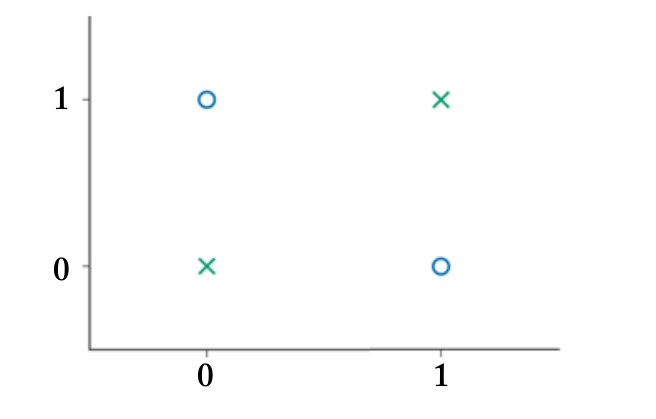
\includegraphics[scale=0.35]{pics/xor.png}
\end{figure}

Es evidente que ninguna línea recta puede separar las dos clases.


\subsection{Transformaciones no lineales de las entradas}
Si transformamos los puntos alimentándolos a través de la función no lineal $\phi(x_1,x_2) = [x_1 \times x_2, x_1 + x_2]$, el problema XOR se vuelve linealmente separable.

\begin{figure}[htb]
	\centering
	 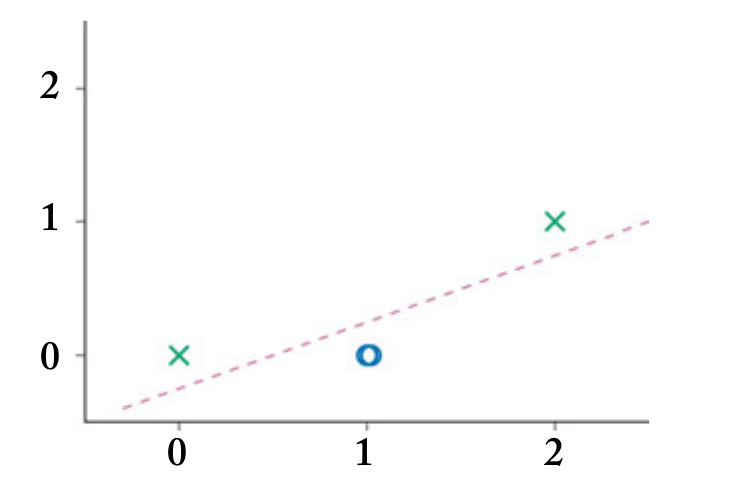
\includegraphics[scale=0.25]{pics/xor2.png}
\end{figure}

La función $\phi$ mapea los datos a una representación adecuada para la clasificación lineal. Ahora podemos entrenar fácilmente un clasificador lineal para resolver el problema XOR.

\begin{equation}
\hat{y} = f(\vec{x}) = \phi(\vec{x}) \cdot \vec{w} + b
\end{equation}

El problema es que necesitamos definir manualmente la función $\phi$. Este proceso depende del conjunto de datos particular y requiere mucha intuición humana. La sol

ción es definir una función de mapeo no lineal entrenable y entrenarla junto con el clasificador lineal. Encontrar la representación adecuada se convierte en responsabilidad del algoritmo de entrenamiento.

Las funciones de mapeo pueden tomar la forma de un modelo lineal parametrizado, seguido de una función de activación no lineal $g$ que se aplica a cada una de las dimensiones de salida:

\begin{equation}
\begin{split}
\hat{y} = f(\vec{x}) = \phi(\vec{x}) \cdot \vec{w} + b \\
\phi(\vec{x}) = g(\vec{x}W' + \vec{b}') \\
\end{split}
\end{equation}

Si tomamos $g(x) = \operatorname{max}(0, x)$ y $W' = \begin{pmatrix}
    1 & 1 \\ 1 & 1 \end{pmatrix}$, $\vec{b}' = \begin{pmatrix}
    -1 & 0 \end{pmatrix}$, obtenemos un mapeo equivalente a $[x_1 \times x_2, x_1 + x_2]$ para nuestros puntos de interés (0,0), (0,1), (1,0) y (1,1). ¡Esto resuelve con éxito el problema XOR!

Aprender tanto la función de representación como el clasificador lineal en la parte superior de ella al mismo tiempo es la idea principal detrás del aprendizaje profundo y las redes neuronales. De hecho, la ecuación anterior describe una arquitectura de red neuronal muy común llamada perceptrón multicapa (MLP, por sus siglas en inglés).



\chapter{Redes Neuronales}
\label{cap_redes}



%Translate this Latex book chapter to Spanish. Output in Latex format. Rearrange bullet points (\items) into full paragraphs. Make sure that sentences are connected in a more fluid way as they come.

\begin{itemize}
\item Las redes neuronales son una familia muy popular de modelos de aprendizaje automático formados por unidades llamadas \textbf{neuronas}.
\item Una neurona es una unidad computacional que tiene entradas y salidas escalares.
\item Cada entrada tiene asociado un peso $w$.
\item La neurona multiplica cada entrada por su peso y luego los suma (también son posibles otras funciones como \textbf{max}).
\item Aplica una función de activación $g$ (generalmente no lineal) al resultado y lo pasa a su salida.
\item Se pueden apilar múltiples capas.
\item La función de activación no lineal $g$ juega un papel crucial en la capacidad de la red para representar funciones complejas.
\item Sin la no linealidad en $g$, la red neuronal solo puede representar transformaciones lineales de la entrada.
\end{itemize}

Ejemplo: Red feedforward con dos capas

\begin{figure}[htb]
	\centering
	 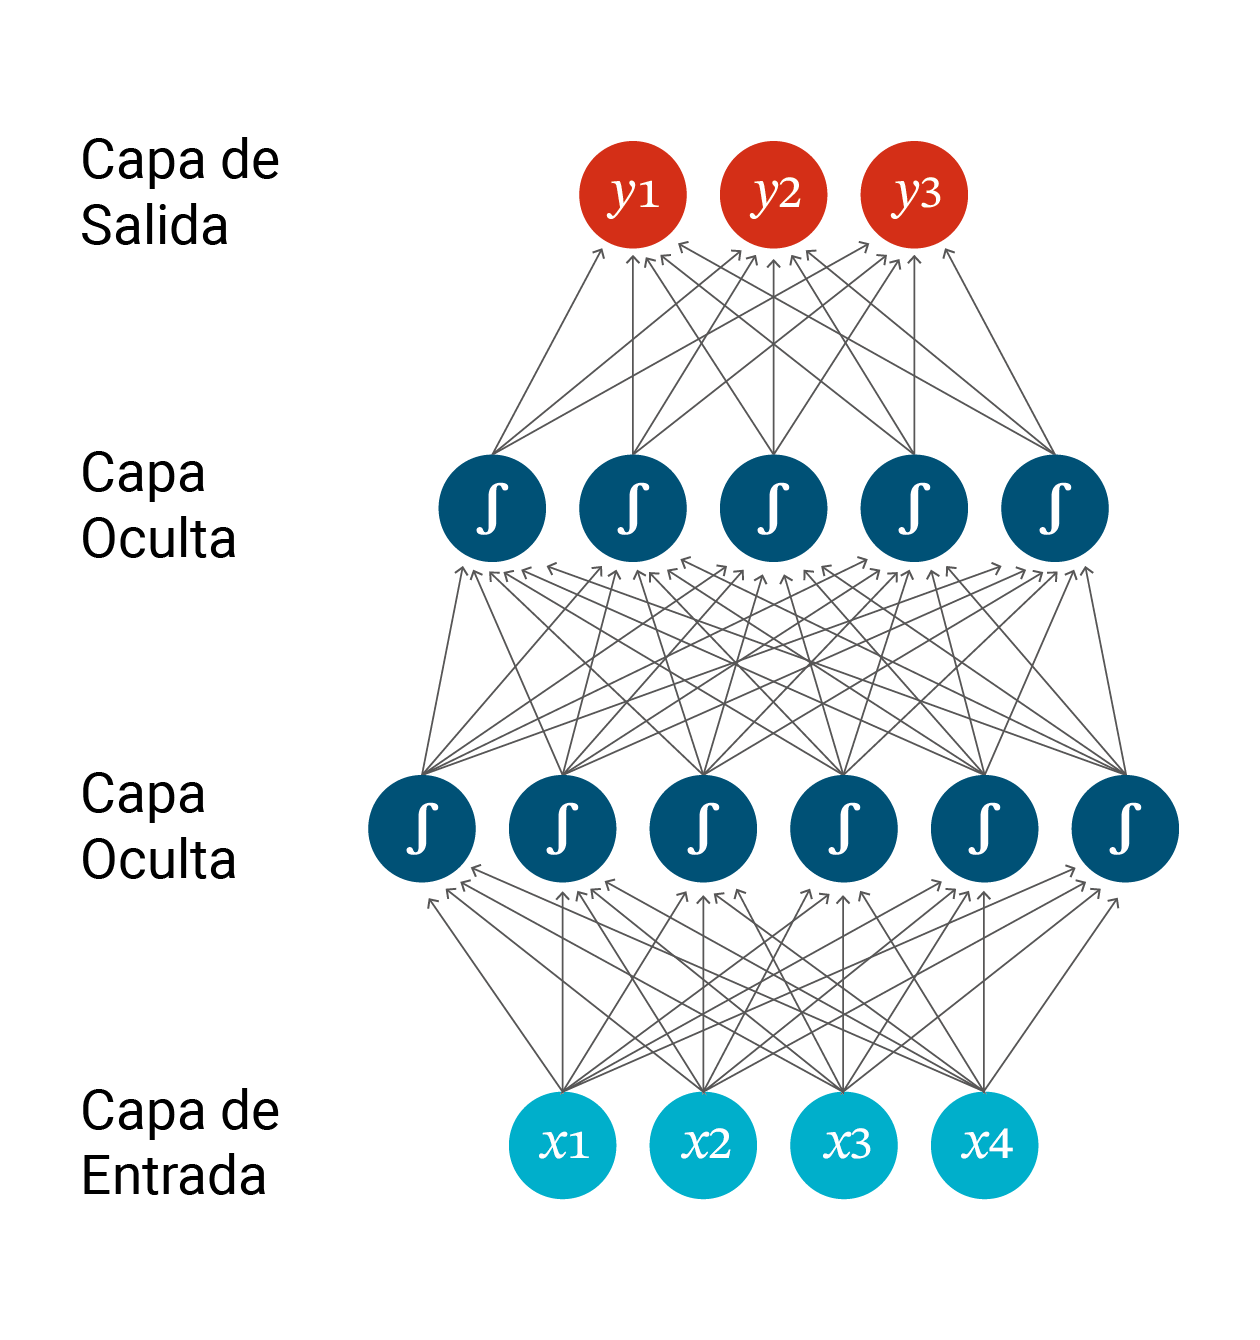
\includegraphics[scale=0.38]{pics/NN-example.png}
\end{figure}

\footnotetext{Fuente:\cite{goldberg2017neural}}

\section{Redes neuronales feedforward}

\begin{itemize}
\item La red feedforward de la imagen es una concatenación de modelos lineales separados por funciones no lineales.
\item Los valores de cada fila de neuronas en la red se pueden pensar como un vector.
\item La capa de entrada es un vector de 4 dimensiones $(\vec{x})$, y la capa superior es un vector de 6 dimensiones $(\vec{h}^1)$.
\item La capa completamente conectada se puede pensar como una transformación lineal de 4 dimensiones a 6 dimensiones.
\item Una capa completamente conectada implementa una multiplicación de vector-matriz, $\vec{h}=\vec{x}W$.
\item El peso de la conexión desde la neurona $i$-ésima en la fila de entrada hasta la neurona $j$-ésima en la fila de salida es $W_{[i,j]}$.
\item Los valores de $\vec{h}$ se transforman mediante una función no lineal $g$ que se aplica a cada valor antes de pasar al siguiente nivel.

\end{itemize}

\footnotetext{Se asume que los vectores son vectores fila y los índices en superíndices corresponden a las capas de la red.}

\paragraph{Capas completamente conectadas como multiplicaciones de vectores y matrices}
\begin{figure}[htb]
	\centering
	 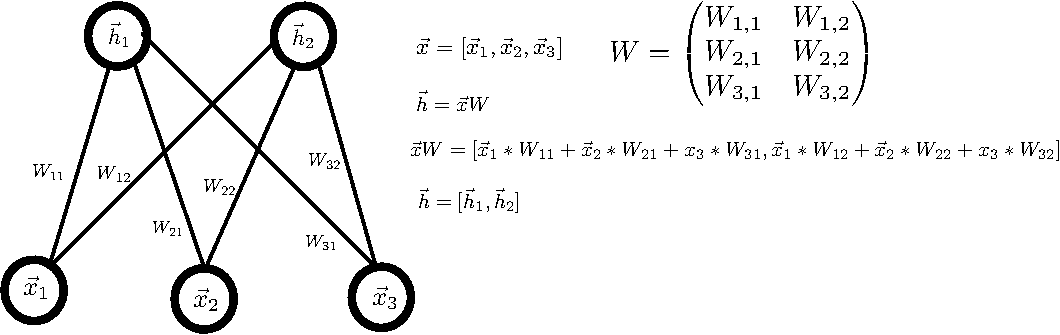
\includegraphics[scale=0.65]{pics/neural_net_mat_mul.pdf}
\end{figure}

\subsection{Redes neuronales como funciones matemáticas}

\begin{itemize}
\item El Perceptrón Multicapa (MLP, por sus siglas en inglés) de la figura se llama MLP2 porque tiene dos capas ocultas.
\item Un modelo más simple sería MLP1, un perceptrón multicapa de una capa oculta:
\begin{center}
\begin{equation}
\begin{split}
\vec{\hat{y}} = NN_{MLP1}(\vec{x}) = g(\vec{x}W^{1}+\vec{b}^{1})W^{2}+\vec{b}^{2} \\
\vec{x} \in \mathcal{R}^{in}, W^{1} \in \mathcal{R}^{d_{in}\times d_{1}}, \vec{b}^{1} \in \mathcal{R}^{d_{1}}, W^{2} \in \mathcal{R}^{d_{1}\times d_{out}}, \vec{b}^{2} \in \mathcal{R}^{d_{out}}, \vec{\hat{y}} \in \mathcal{R}^{d_{out}}
\end{split}
\end{equation}
\end{center}

\item Aquí, $W^{1}$ y $\vec{b}^{1}$ son una matriz y un término de sesgo para la primera transformación lineal de la entrada.
\item La función $g$ es una función no lineal que se aplica elemento a elemento (también se llama no linealidad o función de activación).
\item $W^{2}$ y $\vec{b}^{2}$ son la matriz y el término de sesgo para una segunda transformación lineal.

\item Al describir una red neuronal, se deben especificar las dimensiones de las capas ($d_{1}$), la entrada ($d_{in}$) y la salida ($d_{out}$).
\item MLP2 se puede escribir como la siguiente función matemática:
\begin{center}
\begin{equation}
\begin{split}
NN_{MLP2}(\vec{x}) & =  \vec{\hat{y}}  \\
\vec{h}^{1} &  = \vec{x}W^{1}+\vec{b}^{1} \\
\vec{h}^{2} &  = g^{1}(\vec{h}^{1})W^{2}+\vec{b}^{2} \\
\vec{y} &  = g^{2}(\vec{h}^{2})W^{3}\\
\vec{y} &  = (g^2(g^1(\vec{x}W^{1}+\vec{b}^{1})W^2+\vec{b}^2))W^3.\\
\end{split}
\end{equation}
\end{center}
\item Las matrices y los términos de sesgo que definen las transformaciones lineales son los parámetros de la red.
\item Al igual que en los modelos lineales, es común referirse a la colección de todos los parámetros como $\Theta$.
\end{itemize}

\section{Capacidad de representación}

\begin{itemize}
\item \cite{hornik1989multilayer} y \cite{cybenko1989approximation} mostraron que un perceptrón multicapa de una capa oculta (MLP1) es un aproximador universal.
\item MLP1 puede aproximar todas las funciones continuas en un subconjunto cerrado y acotado de $\mathcal{R}^n$.
\item Esto puede sugerir que no hay razón para ir más allá de MLP1 en arquitecturas más complejas.
\item El resultado no dice qué tan fácil o difícil es establecer los parámetros basándose en los datos de entrenamiento y un algoritmo de aprendizaje específico.
\item Tampoco garantiza que un algoritmo de entrenamiento encontrará la función correcta que genera nuestros

datos de entrenamiento.
\item Finalmente, no establece qué tan grande debería ser la capa oculta.
\item En la práctica, entrenamos redes neuronales con cantidades relativamente pequeñas de datos utilizando métodos de búsqueda local.
\item También utilizamos capas ocultas de tamaños relativamente modestos (hasta varios miles).
\item El teorema de aproximación universal no ofrece ninguna garantía bajo estas condiciones.
\item Sin embargo, definitivamente hay beneficios en probar arquitecturas más complejas que MLP1.
\item En muchos casos, sin embargo, MLP1 brinda resultados sólidos.
\end{itemize}

\section{Funciones de activación}
\begin{itemize}
\item La no linealidad $g$ puede tomar muchas formas.
\item Actualmente no existe una buena teoría sobre qué no linealidad aplicar en qué condiciones.
\item Elegir la no linealidad correcta para una tarea determinada es en su mayor parte una cuestión empírica.
\end{itemize}

\paragraph{Sigmoide}
\begin{itemize}
\item La función de activación sigmoide $\sigma(x) = \frac{1}{1+e^{-x}}$ es una función en forma de S, que transforma cada valor x en el rango $[0, 1]$.
\item El sigmoide fue la no linealidad canónica para las redes neuronales desde su inicio.
\item Actualmente se considera obsoleta para su uso en capas internas de redes neuronales, ya que las opciones que se enumeran a continuación funcionan mucho mejor empíricamente.
\end{itemize}

\begin{figure}[htb]
	\centering
	 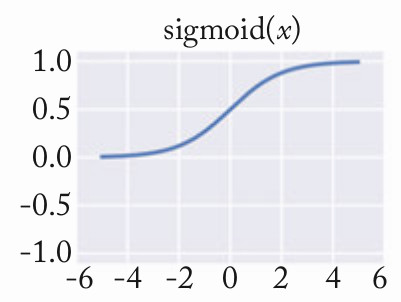
\includegraphics[scale=0.3]{pics/sigmoid2.png}
\end{figure}

\paragraph{Tangente hiperbólica (tanh)}
\begin{itemize}
\item La función de activación tangente hiperbólica $\operatorname{tanh}(x) = \frac{e^{2x}-1}{e^{2x}+1}$ es una función en forma de S que transforma los valores x en el rango $[-1, 1]$.
\end{itemize}

\begin{figure}[htb]
	\centering
	 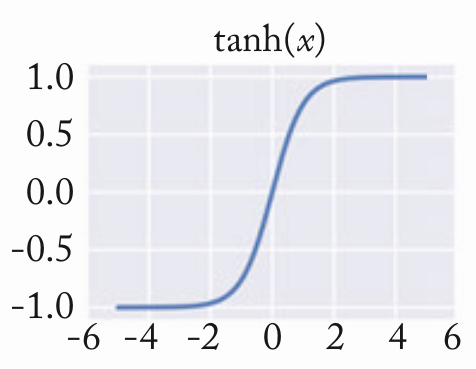
\includegraphics[scale=0.3]{pics/tanh.png}
\end{figure}

\paragraph{Hard tanh}
\begin{itemize}
\item La función de activación hard-tanh es una aproximación de la función tangente hiperbólica que es más rápida de calcular y encontrar sus derivadas:
\end{itemize}

  \[
    \operatorname{hardtanh}(x) = \left\{\begin{array}{lr}
        -1 & x < -1\\
        1 & x > 1\\
        x & \text{en otros casos.}
        \end{array} \right\}
  \]

\begin{figure}[htb]
	\centering
	 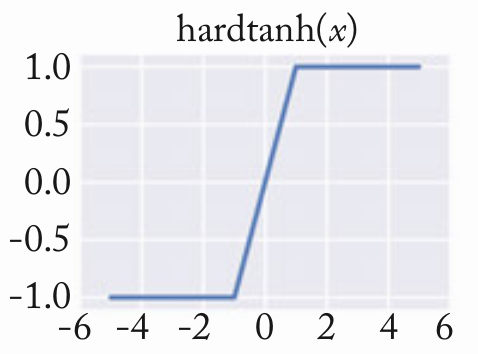
\includegraphics[scale=0.3]{pics/hardtanh.png}
\end{figure}

\paragraph{ReLU}
\begin{itemize}
\item La función de activación rectificador \cite{glorot2011deep}, también conocida como unidad lineal rectificada, es una función de activación muy simple.
\item Es fácil de trabajar y se ha demostrado muchas veces que produce excelentes resultados.
\item La

función ReLU se define como $ReLU(x) = \max(0, x)$.
\end{itemize}

\begin{figure}[htb]
	\centering
	 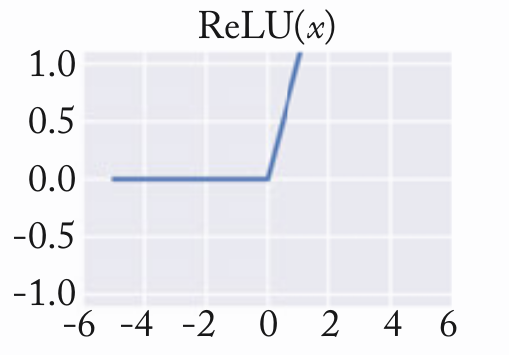
\includegraphics[scale=0.3]{pics/relu.png}
\end{figure}

\paragraph{Leaky ReLU}
\begin{itemize}
\item La función Leaky ReLU es similar a ReLU, pero permite una pequeña pendiente para valores negativos.
\item Se define como $LeakyReLU(x) = \max(\alpha x, x)$, donde $\alpha$ es un hiperparámetro pequeño (por lo general, en el rango de $0.01$ a $0.2$).
\end{itemize}

%\begin{figure}[htb]
%	\centering
%	 \includegraphics[scale=0.3]{pics/leakyrelu.png}
%\end{figure}

\paragraph{ELU}
\begin{itemize}
\item La función de activación ELU (Exponential Linear Unit) \cite{clevert2015fast} es una versión mejorada de ReLU que también tiene una pendiente para valores negativos.
\item Se define como $ELU(x) = \left\{\begin{array}{lr}
        \alpha (e^x - 1) & x < 0\\
        x & \text{en otros casos.}
        \end{array} \right\}$
\item Aquí, $\alpha$ es un hiperparámetro que controla la pendiente negativa.
\end{itemize}

%\begin{figure}[htb]
%	\centering
%	 \includegraphics[scale=0.3]{pics/elu.png}
%\end{figure}

Estas son solo algunas de las muchas opciones disponibles para las funciones de activación en redes neuronales. La elección de la función de activación puede depender del problema específico y puede requerir pruebas empíricas para determinar cuál funciona mejor.



\subsection{Problemas Prácticos}
En términos generales, tanto las unidades ReLU como las unidades tangente hiperbólica (tanh) funcionan bien y superan significativamente a la función sigmoide. Sin embargo, puede ser beneficioso experimentar con ambas activaciones, ya que cada una puede funcionar mejor en diferentes configuraciones. La Figura 1 muestra las formas de las diferentes funciones de activación, junto con las formas de sus derivadas.

\begin{figure}[htb]
	\centering
	 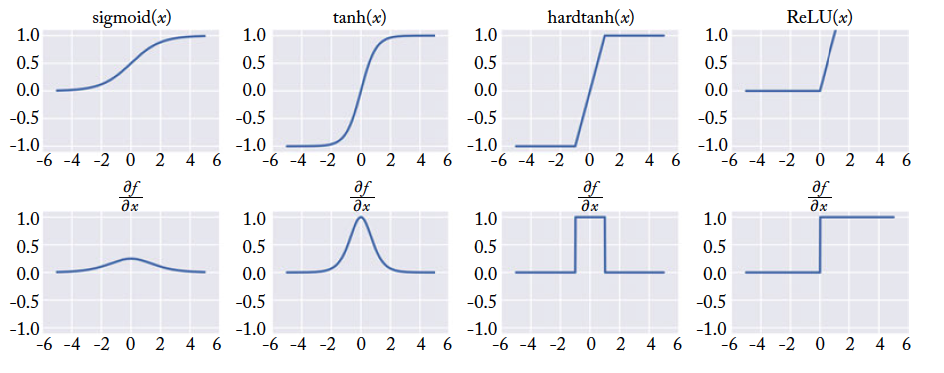
\includegraphics[scale=0.35]{pics/activations.png}
\end{figure}

\footnotetext{Fuente:\cite{goldberg2017neural}}

\section{Capas de Embedding}
En el procesamiento del lenguaje natural (PLN), la entrada a la red neuronal contiene características categóricas simbólicas (por ejemplo, palabras de un vocabulario cerrado, n-gramas de caracteres, etiquetas POS). En los modelos lineales, generalmente representamos la entrada con vectores dispersos, como la suma, el promedio o la concatenación de vectores codificados one-hot (la suma o el promedio pueden producir una representación de bolsa de palabras). En las redes neuronales, es común asociar cada valor de característica posible (es decir, cada palabra en el vocabulario, cada categoría de etiqueta POS) con un vector denso de $d$ dimensiones.

Estos vectores luego se consideran parámetros del modelo y se entrenan conjuntamente con los demás parámetros. El mapeo desde valores de características simbólicas, como "número de palabra 1249", a vectores de $d$ dimensiones se realiza mediante una capa de embedding (también llamada capa de búsqueda). Los parámetros en una capa de embedding de palabras son simplemente una matriz $E \in \mathbb{R}^{|vocab|\times d}$ donde cada fila corresponde a una palabra diferente en el vocabulario. La operación de búsqueda es simplemente una indexación: $v_{1249} = E_{[1249,:]}$. Si la característica simbólica se codifica como un vector one-hot $\vec{x}$, la operación de búsqueda se puede implementar como una multiplicación de matriz-vector $\vec{x}E$. Los vectores de embedding se combinan antes de pasar a la siguiente capa. Las operaciones comunes de combinación son concatenación, suma y promedio. Una matriz de embeddings de palabras $E$ se puede inicializar con vectores de palabras preentrenados a partir de documentos no etiquetados utilizando métodos específicos basados en la hipótesis distribucional, como los implementados en Word2Vec (que se discutirán más adelante en el curso).

\begin{figure}[htb]
	\centering
	 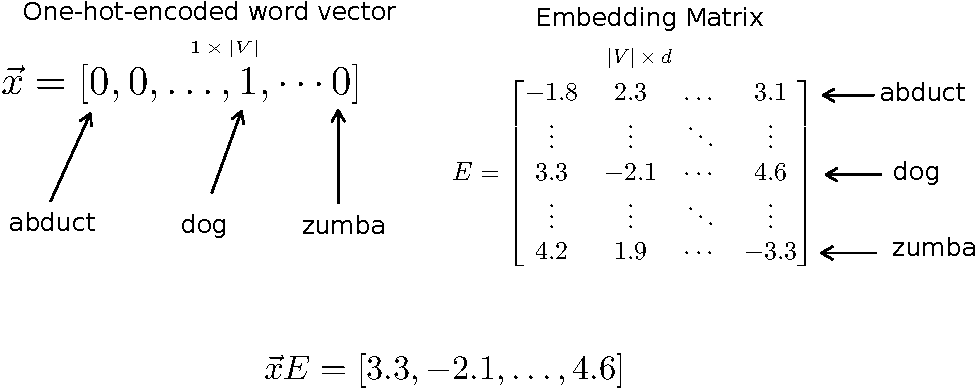
\includegraphics[scale=0.65]{pics/emb_matrix.pdf}
\end{figure}

\subsection{Vectores Densos vs Representaciones One-hot}
¿Cuáles son los beneficios de representar nuestras características como vectores en lugar de como identificadores únicos? ¿Deberíamos siempre representar las características como vectores densos? Consideremos los dos tipos de representaciones.

\begin{enumerate}
 \item \textbf{One Hot}: cada característica es su propia dimensión.
 \begin{itemize}
  \item La dimensionalidad del vector one-hot es igual al número de características distintas.
  \item  Las características son completamente independientes entre sí. La característica "la palabra es 'perro'" es tan diferente de "la palabra es 'pensando'" como lo es de "la palabra es 'gato'".
 \end{itemize}
\item \textbf{Dense}: cada característica es un vector de d dimensiones.
\begin{itemize}
 \item La dimensionalidad del vector es d.
 \item El entrenamiento del modelo hará que características similares tengan vectores similares: la información se comparte entre características similares.
\end{itemize}
\end{enumerate}




\paragraph{Ejemplo: Vectores Densos vs Representaciones One-hot}

\begin{figure}[htb]
	\centering
	 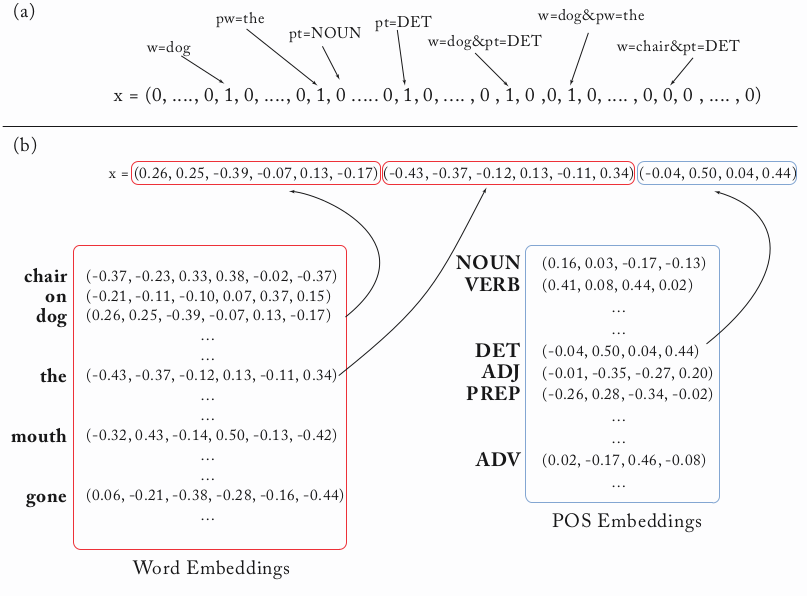
\includegraphics[scale=0.35]{pics/denseonehot.png}
\end{figure}

La figura anterior muestra dos codificaciones de la información: la palabra actual es "perro"; la palabra anterior es "el"; la etiqueta POS anterior es "DET".

(a) Vector de características dispersas:
\begin{itemize}
 \item Cada dimensión representa una característica.
\item Las combinaciones de características tienen sus propias dimensiones.
\item Los valores de las características son binarios.
\item La dimensionalidad es muy alta.
\end{itemize}


(b) Vector de características densas basado en embeddings.

\begin{itemize}
\item Cada característica principal se representa como un vector.
\item  Cada característica se corresponde con varias entradas del vector de entrada.
\item No hay una codificación explícita de combinaciones de características.
\item La dimensionalidad es baja.
\item Los mapeos de características a vectores provienen de una tabla de embeddings.
\end{itemize}


Un beneficio de usar vectores densos y de baja dimensionalidad es computacional: la mayoría de las bibliotecas de redes neuronales no funcionan bien con vectores dispersos de alta dimensionalidad. Sin embargo, este es solo un obstáculo técnico que se puede resolver con cierto esfuerzo de ingeniería.

El principal beneficio de las representaciones densas radica en el poder de generalización. Si creemos que algunas características pueden proporcionar pistas similares, vale la pena proporcionar una representación que pueda capturar estas similitudes. Supongamos que hemos observado la palabra "perro" muchas veces durante el entrenamiento, pero solo hemos observado la palabra "gato" unas pocas veces. Si cada una de las palabras se asocia con su propia dimensión (one-hot), las ocurrencias de "perro" no nos dirán nada sobre las ocurrencias de "gato". Sin embargo, en la representación de vectores densos, el vector aprendido para "perro" puede ser similar al vector aprendido para "gato". Esto permitirá que el modelo comparta fuerza estadística entre los dos eventos. Este argumento asume que hemos visto suficientes ocurrencias de la palabra "gato" como para que su vector sea similar al de "perro". Los vectores de palabras preentrenados (por ejemplo, Word2Vec, GloVe), que se discutirán más adelante en el curso, se pueden utilizar para obtener vectores densos a partir de texto no anotado.



\section{Entrenamiento de Redes Neuronales}

Las redes neuronales se entrenan de la misma manera que los modelos lineales. La salida de la red se utiliza para calcular una función de pérdida $L(\hat{y},y)$ que se minimiza en todos los ejemplos de entrenamiento utilizando descenso de gradiente. El algoritmo de retropropagación es una técnica eficiente para evaluar el gradiente de una función de pérdida $L$ en una red neuronal de alimentación directa con respecto a todos sus parámetros (Bishop, 2006). Los parámetros de la red incluyen $W^1, \vec{b}^1, \dots, W^m, \vec{b}^m$ para una red de $m$ capas. Cabe destacar que los superíndices se utilizan para denotar los índices de las capas (no exponenciación). Para simplificar, asumiremos que $L$ se calcula sobre un solo ejemplo. El desafío radica en que en las redes neuronales el número de parámetros puede ser enorme y necesitamos una forma eficiente de calcular los gradientes. La idea es aplicar la regla de la cadena de derivadas de manera inteligente.

\begin{figure}[htb]
	\centering
	 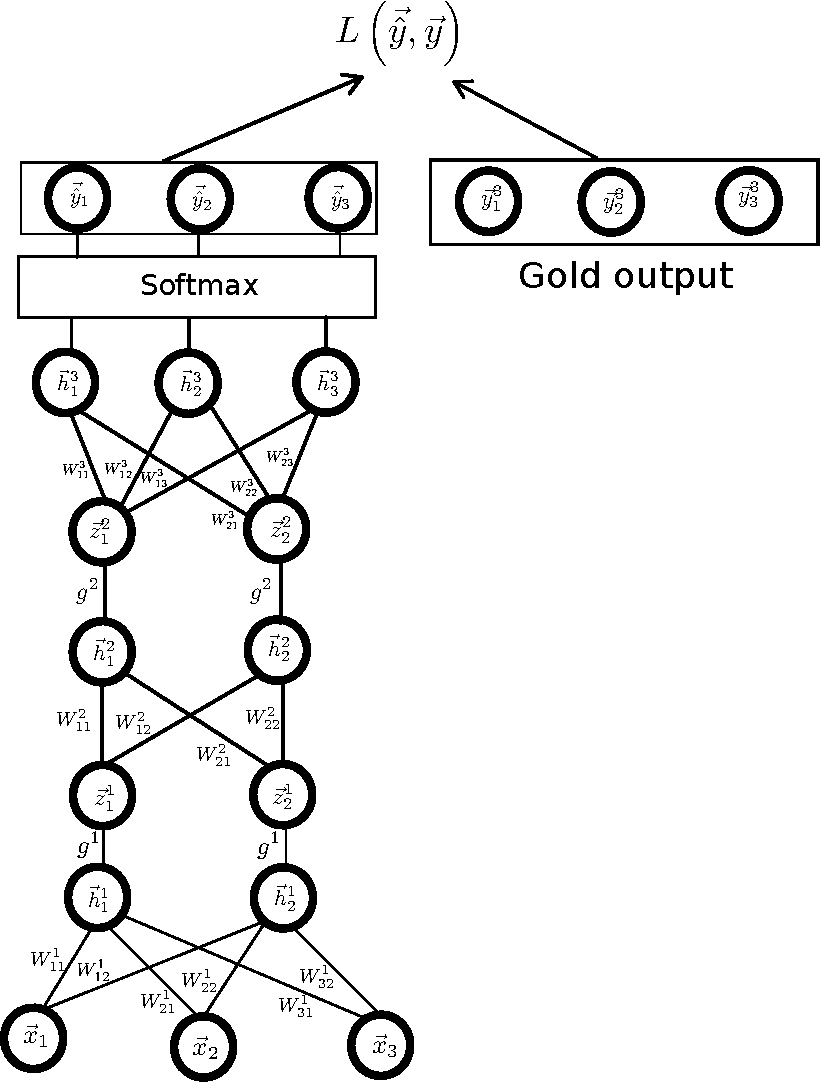
\includegraphics[scale=0.41]{pics/neural_net.pdf}
\end{figure}

\section{Recordatorio de la Regla de la Cadena en Derivadas}

La regla de la cadena simple establece que si $z = f(y)$ y $y = g(x)$, entonces

\begin{displaymath}
\frac{\partial z}{\partial x} = \frac{\partial z}{\partial y} \times \frac{\partial y}{\partial x}
\end{displaymath}

Por ejemplo, si $z= e^{y}$ y $y = 2x$, entonces

\begin{displaymath}
\frac{\partial z}{\partial x} = \frac{\partial z}{\partial y} \times \frac{\partial y}{\partial x} = e^{y} \times 2 = 2 e^{2x}
\end{displaymath}

\begin{figure}[htb]
	\centering
	 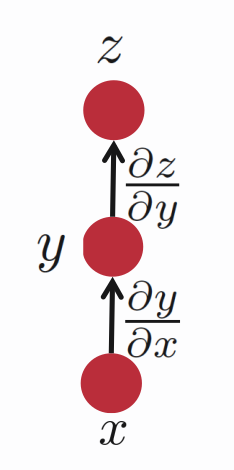
\includegraphics[scale=0.2]{pics/simple_chain_rule.png}
\end{figure}

La regla de la cadena múltiple establece que si $z = f(y_1,y_2)$, $y_1 = g_1(x)$ y $y_2 = g_2(x)$, entonces

\begin{displaymath}
\frac{\partial z}{\partial x} = \frac{\partial z}{\partial y_1} \times \frac{\partial y_1}{\partial x} + \frac{\partial z}{\partial y_2} \times \frac{\partial y_2}{\partial x}
\end{displaymath}

Por ejemplo, si $z= e^{y_1 \times y_2}$, $y_1 = 2x$ y $y_2 = x^2$, entonces

\begin{displaymath}
\frac{\partial z}{\partial x} = (e^{y_1 \times y_2}\times y_2) \times 2 + (e^{y_1 \times y_2}\times y_1) \times 2x = e^{2x^3} \times 6x^2
\end{displaymath}


\begin{figure}[htb]
	\centering
	 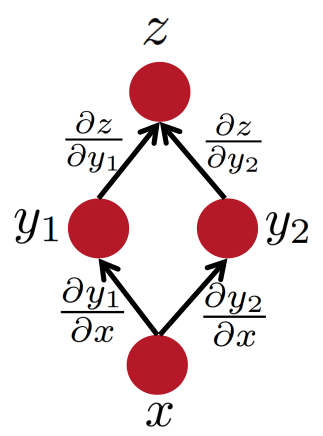
\includegraphics[scale=0.3]{pics/multiple_paths_chain_rule.png}
\end{figure}

La versión general de la regla de la cadena múltiple es:

\begin{displaymath}
 \frac{\partial z}{\partial x} = \sum_{i=1}^n \frac{\partial z}{\partial y_i} \times \frac{\partial y_i}{\partial x}
\end{displaymath}

\begin{figure}[htb]
	\centering
	 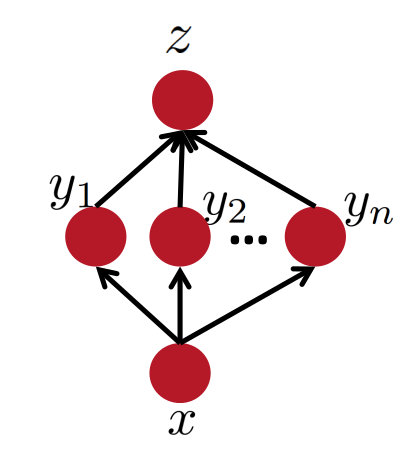
\includegraphics[scale=0.4]{pics/multiple_paths_chain_rule_general.png}
\end{figure}

\section{Retropropagación}

En una red de alimentación directa general, cada unidad calcula una suma ponderada de sus entradas de la siguiente forma:

\begin{equation}
\vec{h}_{[j]}^l = \left(\sum_{i}  W_{[i,j]}^l \times \vec{z}_{[i]}^{(l-1)}\right) + \vec{b}_{[j]}^l
\label{eq:sum}
\end{equation}

La variable $\vec{z}_{[i]}^{(l-1)}$ es una entrada que envía una conexión a la unidad $\vec{h}_{[j]}^l$, $W_{[i,j]}^l$ es el peso asociado con esa conexión, y $l$ es el índice de la capa.

Los vectores de sesgo $\vec{b}_{[j]}$ pueden excluirse de (eq. \ref{eq:sum}) e incluirse en la matriz de pesos $W_{[i,j]}^l$ al introducir una unidad adicional, o entrada, con una activación fija de +1.

Las entradas en la capa $l$, $\vec{z}_{[i]}^{(l-1)}$, son el resultado de aplicar la función de activación $g$ a las unidades de la capa anterior:

\begin{equation}
\vec{z}_{[j]}^{l} = g(\vec{h}_{[j]}^{l})
\label{eq:ac}
\end{equation}

Para la capa de entrada ($l=0$), $\vec{z}$ corresponde al vector de entrada $\vec{z} = \vec{x}$:

\begin{equation}
\vec{z}_{[j]}^0 = \vec{x}_{[j]}
\end{equation}

Para cada instancia en el conjunto de entrenamiento, proporcionamos el vector de entrada correspondiente $\vec{x}$ a la red. Luego calculamos las activaciones de todas las unidades ocultas y de salida en la red mediante la aplicación sucesiva de (eq. \ref{eq:sum}) y (eq. \ref{eq:ac}).

Este proceso a menudo se denomina propagación hacia adelante porque se puede considerar como un flujo de información hacia adelante a través de la red.

Ahora consideremos la evaluación de la derivada de $L$ con respecto a un peso $W_{[i,j]}^l$.

Suponiendo que la pérdida $L$ se calcula sobre un solo ejemplo, podemos observar que $L$ depende del peso $W_{[i,j]}^l$ únicamente a través de la suma de las entradas $\vec{h}_{[j]}^{l}$.

Por lo tanto, podemos aplicar la

regla de la cadena para derivadas parciales para obtener:

\begin{equation}
\frac{\partial L}{\partial W_{[i,j]}^l} = \frac{\partial L}{\partial \vec{h}_{[j]}^{l}} \times \frac{\partial \vec{h}_{[j]}^{l}}{\partial W_{[i,j]}^l}
\label{eq:chain}
\end{equation}

Ahora introducimos una notación útil:

\begin{equation}
\vec{\delta}_{[j]}^l \equiv \frac{\partial L}{\partial \vec{h}_{[j]}^l}
\label{eq:delta}
\end{equation}

Usando (\ref{eq:sum}), podemos escribir

\begin{equation}
\frac{\partial \vec{h}_{[j]}^l}{\partial W_{[i,j]}^l} = \vec{z}_{[i]}^{(l-1)}
\label{eq:part}
\end{equation}

Sustituyendo (\ref{eq:delta}) y (\ref{eq:part}) en (\ref{eq:chain}), obtenemos

\begin{equation}
\frac{\partial L}{\partial W_{[i,j]}^l} = \vec{\delta}_{[j]}^l \times \vec{z}_{[i]}^{(l-1)}
\label{eq:deltarule}
\end{equation}

La ecuación (\ref{eq:deltarule}) nos dice que la derivada requerida se obtiene simplemente multiplicando el valor de $\vec{\delta}_{[j]}^l$ por el valor de $\vec{z}_{[i]}^{(l-1)}$.

Por lo tanto, para evaluar las derivadas, solo necesitamos calcular el valor de $\vec{\delta}_{[j]}^l$ para cada unidad oculta y de salida en la red, y luego aplicar (\ref{eq:deltarule}) para actualizar los pesos de la red. Este proceso se conoce como retropropagación, ya que el cálculo del gradiente se propaga hacia atrás a través de la red.


Calcular $\vec{\delta}_{[j]}^m$ para las unidades de salida ($l=m$) suele ser directo, ya que las unidades de activación $\vec{h}_{[j]}^m$ se observan directamente en la expresión de pérdida.

Lo mismo se aplica a los modelos lineales poco profundos.

Para evaluar $\vec{\delta}_{[j]}^l$ para las unidades ocultas, nuevamente hacemos uso de la regla de la cadena para derivadas parciales:

\begin{equation}
\vec{\delta}_{[j]}^l \equiv \frac{\partial L}{\partial \vec{h}_{[j]}^l} = \sum_{k}\left( \frac{\partial L}{\partial \vec{h}_{[k]}^{l+1}} \times \frac{\partial \vec{h}_{[k]}^{l+1}}{\partial \vec{h}_{[j]}^l}\right)
\label{eq:deltachain}
\end{equation}

La suma se realiza sobre todas las unidades $\vec{h}_{[k]}^{l+1}$ a las que la unidad $\vec{h}_{[j]}^l$ envía conexiones.

Suponemos que las conexiones se realizan solo entre capas consecutivas en la red (desde la capa $l$ hasta la capa $(l+1)$).

Las unidades $\vec{h}_{[k]}^{l+1}$ podrían incluir otras unidades ocultas y/o unidades de salida.

Si ahora sustituimos la definición de $\vec{\delta}_{[j]}^l$ dada por la ecuación (\ref{eq:delta}) en la ecuación (\ref{eq:deltachain}), obtenemos:

\begin{equation}
\vec{\delta}_{[j]}^l \equiv \frac{\partial L}{\partial \vec{h}_{[j]}^l} = \sum_{k}\left( \vec{\delta}_{[k]}^{(l+1)}  \times \frac{\partial \vec{h}_{[k]}^{l+1}}{\partial \vec{h}_{[j]}^l} \right)
\label{eq:delta2}
\end{equation}

Ahora, para la expresión $\vec{h}_{[k]}^{l+1}$ podemos ir a su definición (ecuación \ref{eq:sum}):

\begin{displaymath}
\vec{h}_{[k]}^{(l+1)} = \left( \sum_{i} W_{[i,k]}^{l+1} \times \vec{z}_{[i]}^{l}\right) + \vec{b}_{[k]}^{(l+1)}
\end{displaymath}

Reemplazando ahora la ecuación (\ref{eq:ac}) $(\vec{z}_{[i]}^{l} = g(\vec{h}_{[i]}^{l}))$ en la ecuación anterior, obtenemos:

\begin{displaymath}
\vec{h}_{[k]}^{(l+1)} = \left( \sum_{i}   W_{[i,k]}^{l+1} \times g(\vec{h}_{[i]}^{l})\right)  + \vec{b}_{[k]}^{(l+1)}
\end{displaymath}

Al calcular $\frac{\partial \vec{h}_{[k]}^{l+1}}{\partial \vec{h}_{[j]}^l}$, todos los términos en la suma donde $i \neq j$ se cancelan.

Por lo tanto, tenemos:

\begin{equation}
\frac{\partial \vec{h}_{[k]}^{l+1}}{\partial \vec{h}_{[j]}^l} =  W_{[j,k]}^{l+1} \times g'(\vec{h}_{[j]}^{l})
\label{eq:partialhh}
\end{equation}

Sustituyendo la ecuación (\ref{eq:partialhh}) en la ecuación (\ref{eq:delta2}), obtenemos:

\begin{equation}
\vec{\delta}_{[j]}^l \equiv \frac{\partial L}{\partial \vec{h}_{[j]}^l} = \sum_{k} \left( \vec{\delta}_{[k]}^{(l+1)}  \times W_{[j,k]}^{l+1} \times g'(\vec{h}_{[j]}^{l}) \right)
\label{eq:delta3}
\end{equation}

Dado que $g'(\vec{h}_{[j]}^{l})$ no depende de $k$, podemos obtener la siguiente fórmula de retropropagación:

\begin{equation}
\vec{\delta}_{[j]}^l = g'(\vec{h}_{[j]}^{l}) \times \sum_{k} \left( \vec{\delta}_{[k]}^{(l+1)}  \times W_{[j,k]}^{l+1}\right)
\label{eq:delta4}
\end{equation}

Esto nos dice que el valor de $\vec{\delta}$ para una unidad oculta en particular se puede obtener propagando los $\vec{\delta}$ hacia atrás desde las unidades superiores en la red \cite{bishop2006pattern}.

El procedimiento de retropropagación se puede resumir de la siguiente manera:

\begin{enumerate}
  \item Aplicar un vector de entrada $\vec{x}$ a la red y propagarlo hacia adelante a través de la red utilizando las ecuaciones (\ref{eq:sum}) y (\ref{eq:ac}) para encontrar las activaciones de todas las unidades ocultas y de salida.
  \item Calcular $\vec{\delta}_{[j]}^m$ para todas las unidades de salida (recordar que las derivadas involucradas aquí son fáciles de calcular).
  \item Retropropagar los $\vec{\delta}_{[k]}^{(l+1)}$ utilizando la ecuación (\ref{eq:delta4}) para obtener $\vec{\delta}_{[j]}^l$ para cada unidad oculta en la red. Se realiza de capas superiores a capas inferiores en la red.
  \item Utilizar la ecuación (\ref{eq:deltarule}) $(\frac{\partial L}{\partial W_{[i,j]}^l} = \vec{\delta}_{[j]}^l \times \vec{z}_{[i]}^{(l-1)})$ para evaluar las derivadas requeridas.
\end{enumerate}
\section{La Abstracción del Grafo de Cómputo}
Uno puede calcular los gradientes de los varios parámetros de una red a mano e implementarlos en código. Sin embargo, este procedimiento es engorroso y propenso a errores. Por lo tanto, para la mayoría de los propósitos, es preferible utilizar herramientas automáticas para el cálculo de gradientes \cite{bengio2012practical}.

Una representación de una computación matemática arbitraria (por ejemplo, una red neuronal) como un grafo es llamada un grafo de cómputo. Esta abstracción nos permite calcular los gradientes para cualquier tipo de arquitectura de red neuronal utilizando el algoritmo de retropropagación. La formulación anterior estaba restringida a redes feedforward.

Un grafo de cómputo es un grafo dirigido acíclico (DAG, por sus siglas en inglés). Los nodos corresponden a operaciones matemáticas o variables (ligadas), y las aristas corresponden al flujo de valores intermedios entre los nodos. La estructura del grafo define el orden de la computación en términos de las dependencias entre los diferentes componentes. Dado que el resultado de una operación puede ser la entrada de varias continuaciones, el grafo es un DAG y no un árbol.

Consideremos, por ejemplo, un grafo para el cálculo de $(a*b+1)*(a*b+2)$:

\begin{figure}[htb]
	\centering
	 \includegraphics[scale=0.25]{pics/compGraph.png}
\end{figure}

La computación de $a*b$ es compartida. Dado que una red neuronal es esencialmente una expresión matemática, se puede representar como un grafo de cómputo.

La figura anterior muestra el grafo de cómputo para una MLP con una capa oculta y una transformación de salida softmax \cite{goldberg2017neural}. Los nodos ovalados representan operaciones matemáticas o funciones, y los nodos rectangulares sombreados representan parámetros (variables ligadas). Las entradas de la red se tratan como constantes y se dibujan sin un nodo circundante. Los nodos de entrada y parámetros no tienen aristas de entrada, y los nodos de salida no tienen aristas de salida. La salida de cada nodo es una matriz, cuya dimensionalidad se indica sobre el nodo.

Este grafo es incompleto: sin especificar las entradas, no podemos calcular una salida. La figura 5.1b muestra un grafo completo para una MLP que toma tres palabras como entradas y predice la distribución de etiquetas gramaticales para la tercera palabra. Este grafo se puede utilizar para la predicción, pero no para el entrenamiento, ya que la salida es un vector (no un escalar) y el grafo no tiene en cuenta la respuesta correcta ni el término de pérdida. Finalmente, el grafo en la figura 5.1c muestra el grafo de cómputo para un ejemplo de entrenamiento específico, en el cual las entradas son las (incrustaciones de) las palabras "the", "black", "dog", y la salida esperada es "NOUN" (cuyo índice es 5). El nodo de selección implementa una operación de indexación, recibiendo un vector y un índice (en este caso, 5) y devolviendo la entrada correspondiente en el vector.

\subsection{Cómputo hacia Adelante}
El paso hacia adelante (forward pass) calcula las salidas de los nodos en el grafo. Dado que la salida de cada nodo depende únicamente de sí mismo y de las aristas entrantes, es trivial calcular las salidas de todos los nodos.

Esto se hace recorriendo los nodos en un orden topológico y calculando la salida de cada nodo dado que las salidas de sus predecesores ya han sido calculadas.

Más formalmente, en un grafo de $N$ nodos, asociamos a cada nodo un índice $i$ de acuerdo con su orden topológico. Sea $f_i$ la función calculada por el nodo $i$ (por ejemplo, multiplicación, suma, etc.). Sea $\pi(i)$ los nodos padres del nodo $i$, y $\pi^{-1}(i) = \{j | i \in \pi(j)\}$ los nodos hijos del nodo $i$ (estos son los argumentos de $f_i$). Denotemos por $v(i)$ la salida del nodo $i$, es decir, la aplicación de $f_i$ a los valores de salida de sus argumentos $\pi^{-1}(i)$. Para los nodos de variables e entrada, $f_i$ es una función constante y $\pi^{-1}(i)$ está vacío. El paso hacia adelante en el grafo de cómputo calcula los valores $v(i)$ para todos los $i \in [1,N]$.

\begin{figure}[htb]
	\centering
	 \includegraphics[scale=0.35]{pics/forwardPass.png}
\end{figure}

\subsection{Cómputo hacia Atrás (Retropropagación)}
El paso hacia atrás (backward pass) comienza designando un nodo $N$ con una salida escalar $(1 \times 1)$ como nodo de pérdida y ejecutando el cómputo hacia adelante hasta ese nodo.

El cómputo hacia atrás calcula los gradientes de los parámetros con respecto al valor de ese nodo.

Denotemos por $d(i)$ la cantidad $\frac{\partial N}{\partial i}$. El algoritmo de retropropagación se utiliza para calcular los valores $d(i)$ para todos los nodos $i$.

El paso hacia atrás llena una tabla de valores $d(1), \dots, d(N)$ como se muestra en el siguiente algoritmo.

\begin{figure}[htb]
	\centering
	 \includegraphics[scale=0.35]{pics/backwardPass.png}
\end{figure}

El algoritmo de retropropagación sigue esencialmente la regla de la cadena de la diferenciación. La cantidad $\frac{\partial f_j}{\partial i}$ es la derivada parcial de $f_j(\pi^{-1}(j))$ con respecto al argumento $i \in \pi^{-1}(j)$. Este valor depende de la función $f_j$ y los valores $v(a_1), \dots, v(a_m)$ (donde $a_1, \dots, a_m = \pi^{-1}(j)$) de sus argumentos, los cuales fueron calculados en el paso hacia adelante.

Por lo tanto, para definir un nuevo tipo de nodo, es necesario definir dos métodos: uno para calcular el valor hacia adelante $v(i)$ basado en las entradas del nodo, y otro para calcular $\frac{\partial f_j}{\partial i}$ para cada $x \in \pi^{-1}(i)$.

\subsection{Resumen de la Abstracción del Grafo de Cómputo}
Observa que la formulación anterior de la retropropagación es equivalente a la dada anteriormente en clase.

La abstracción del grafo de cómputo nos permite:

\begin{enumerate}
  \item Construir fácilmente redes arbitrarias.
  \item Evaluar sus predicciones para entradas dadas (paso hacia adelante).
  \item Calcular gradientes para sus parámetros con respecto a pérdidas escalares arbitrarias (paso hacia atrás o retropropagación).
\end{enumerate}

Una propiedad interesante de la abstracción del grafo de cómputo es que nos permite calcular los gradientes para redes arbitrarias (por ejemplo, redes con conexiones saltadas, pesos compartidos, funciones de pérdida especiales, etc.).

\footnotetext{Un tutorial completo sobre el algoritmo de retropropagación sobre la abstracción del grafo de cómputo se puede encontrar aquí: \url{https://colah.github.io/posts/2015-08-Backprop/}.}

\subsection{Derivadas de funciones no matemáticas}
Definir $\frac{\partial f_j}{\partial i}$ para funciones matemáticas como $log$ o $+$ es sencillo.

Puede resultar desafiante pensar en la derivada de operaciones como pick($\vec{x},5$), que selecciona el quinto elemento de un vector.

La respuesta es pensar en términos de la contribución al cálculo. Después de seleccionar el elemento $i$-ésimo de un vector, solo ese elemento participa en el resto del cálculo.

Por lo tanto, el gradiente de pick($\vec{x},5$) es un vector $\vec{v}$ con la dimensionalidad de $\vec{x}$ donde $\vec{v}_{[5]} = 1$ y $\vec{v}_{[i \neq 5]} = 0$.

De manera similar, para la función $\max(0,x)$, el valor del gradiente es $1$ para $x > 0$ y $0$ en caso contrario.

\section{Regularización y Dropout}
Las redes de múltiples capas pueden ser grandes y tener muchos parámetros, lo que las hace especialmente propensas al sobreajuste.

La regularización del modelo es tan importante en las redes neuronales profundas como lo es en los modelos lineales, tal vez incluso más.

Las regularizaciones discutidas para modelos lineales, es decir, $L_2$, $L_1$ y la elastic-net, también son relevantes para las redes neuronales.

Otra técnica efectiva para evitar que las redes neuronales sobreajusten los datos de entrenamiento es el \textbf{dropout training} \cite{srivastava2014dropout}.

El método de dropout está diseñado para evitar que la red aprenda a depender de unidades o conexiones específicas en el proceso de entrenamiento, lo que ayuda a reducir el sobreajuste.

La idea básica detrás del dropout es apagar aleatoriamente unidades (neuronas) en cada paso de entrenamiento, lo que hace que la red aprenda a ser más robusta y generalice mejor.

El dropout  se puede aplicar a las unidades ocultas (neuronas) y/o a las conexiones entre ellas.

Durante el entrenamiento, en cada paso, se aplica una máscara binaria aleatoria a las unidades o conexiones seleccionadas para el dropout. Las unidades o conexiones que están "apagadas" tienen un valor de cero y no contribuyen al cálculo hacia adelante ni hacia atrás. Solo las unidades o conexiones "encendidas" se utilizan en el cálculo de la predicción y en la retropropagación del error.

Durante la inferencia o evaluación, no se aplica el dropout y todas las unidades o conexiones se utilizan para realizar la predicción.

Es importante destacar que el dropout no es una técnica exclusiva de las redes neuronales, pero ha demostrado ser especialmente efectiva en este contexto debido a la gran cantidad de parámetros y conexiones que suelen tener las redes neuronales profundas.

El valor típico para la tasa de dropout, es decir, la fracción de unidades o conexiones que se apagan en cada paso de entrenamiento, suele ser del orden del 0.2 al 0.5. Sin embargo, el valor óptimo puede variar según el problema y la arquitectura de la red. Por lo tanto, es recomendable experimentar con diferentes tasas de dropout para encontrar la mejor configuración para cada caso.

En resumen, la regularización y el dropout son técnicas efectivas para evitar el sobreajuste en las redes neuronales. Al utilizar regularización, como $L_2$ o $L_1$, se penalizan los grandes valores de los parámetros, lo que ayuda a controlar la complejidad del modelo. El dropout, por otro lado, apaga aleatoriamente unidades o conexiones durante el entrenamiento, lo que promueve la robustez y generalización del modelo. Ambas técnicas pueden utilizarse en conjunto para obtener mejores resultados en la generalización y evitar el sobreajuste.


%Translate this Latex book chapter to Spanish. Output in Latex format. Rearrange bullet points (\items) into full paragraphs. Make sure that sentences are connected in a more fluid way as they come.

\section{Frameworks de Aprendizaje Profundo}
Existen varios paquetes de software que implementan el modelo de grafo de cómputo. Todos estos paquetes admiten todos los componentes esenciales (tipos de nodos) para definir una amplia gama de arquitecturas de redes neuronales.

Uno de estos paquetes es \textbf{TensorFlow} (\url{https://www.tensorflow.org/}), una biblioteca de software de código abierto para cálculos numéricos utilizando gráficos de flujo de datos, desarrollada originalmente por el equipo de Google Brain.

Otro paquete popular es \textbf{Keras}, que es una API de alto nivel para redes neuronales que se ejecuta sobre TensorFlow y otros backends (\url{https://keras.io/}).

También tenemos \textbf{PyTorch}, una biblioteca de aprendizaje automático de código abierto para Python basada en Torch, desarrollada por el grupo de investigación de inteligencia artificial de Facebook. PyTorch admite la construcción de gráficos dinámicos, lo que significa que se crea un grafo de cómputo diferente desde cero para cada muestra de entrenamiento (\url{https://pytorch.org/}).






\bibliography{bio}
\bibliographystyle{apalike}

\end{document}
